%\documentclass[textrefs,review]{nddiss2e}
%\documentclass[textrefs,draft]{nddiss2e}
\documentclass[textrefs,final,noinfo]{nddiss2e}

\usepackage[T1]{fontenc}
\usepackage[version=3]{mhchem}
\usepackage{feynmf}
\usepackage{siunitx}
\usepackage{xspace}

\newcommand{\Lagr}{\mathcal{L}}
\newcommand{\psibar}{\overline{\psi}}
\newcommand{\gammafive}{\gamma_{5}}
\newcommand{\onehalf}{\frac{1}{2}}
\newcommand{\VPhi}{V(\phi_{1}^{2}+\phi_{2}^{2})}

\newcommand{\lumiunit}{cm\ensuremath{^{-2}}s\ensuremath{^{-1}}\xspace}
\newcommand{\microunit}[1]{\ensuremath{\mu}#1\xspace}
\newcommand{\micrometer}{\microunit{m}}

\newcommand{\zeroJets}{\emph{Zero/One Jet}\xspace}
\newcommand{\boosted}{\emph{Boost}\xspace}
\newcommand{\vbf}{\emph{VBF}\xspace}
\newcommand{\wBtag}{\emph{B-Tag}\xspace}
\newcommand{\woBtag}{\emph{Non B-Tag}\xspace}

\newcommand{\ttbar}{t\overline{t}\xspace}

\newcommand{\includefinalditauplot}[4] {
\begin{minipage}[b]{0.45\linewidth} 
\centering
  \includegraphics[width=0.95\textwidth]{plots/plotAHtoMuTauOS_#1_#2_#3_#4.pdf}
\end{minipage}
}

\newcommand{\includeditauplot}[4] {
\begin{minipage}[b]{0.45\linewidth} 
\centering
  \includegraphics[width=0.95\textwidth]{plots/plotAHtoMuTau_#1_#2_#3_#4.pdf}
\end{minipage}
}

\newcommand{\includefullplot}[3]{
\centering
  \includegraphics[width=0.95\textwidth]{plots/plotAHtoMuTauOS_#1_finalSamplePlots_#2_#3.pdf}
}

\newcommand{\includeplot}[3]{
\begin{minipage}[b]{0.5\linewidth} 
\centering
  \includegraphics[width=0.95\textwidth]{plots/plotAHtoMuTauOS_#1_finalSamplePlots_#2_#3.pdf}
\end{minipage}
}

\newcommand{\includeleptonplot}[4]{
\begin{minipage}[b]{0.5\linewidth} 
\centering
  \includegraphics[width=0.95\textwidth]{plots/plotAHtoMuTauOS_#1_finalSamplePlots_#2_#3_#4.pdf}
%\includegrahphics[scale=0.35]{plots/plotAHtoMuTauOS_#1_finalSamplePlots_#2_#3_#4.pdf} 
\end{minipage}
}

\newcommand{\includeleptoncutplot}[5]{
\begin{minipage}[b]{0.45\linewidth} 
\centering
  \includegraphics[width=0.95\textwidth]{plots/plotAHtoMuTau_#1_#2_#3_#4_#5.pdf}
%\includegrahphics[scale=0.35]{plots/plotAHtoMuTauOS_#1_finalSamplePlots_#2_#3_#4.pdf} 
\end{minipage}
}

\newcommand{\includebackgroundtemplate}[3]{
\begin{minipage}[b]{0.45\linewidth} 
\centering
  \includegraphics[width=0.95\textwidth]{plots/plotBgEstTemplate#1_vs_AnalysisZtoMuTau_#2_Mass_#3.pdf}
%\includegrahphics[scale=0.35]{plots/plotAHtoMuTauOS_#1_finalSamplePlots_#2_#3_#4.pdf} 
\end{minipage}
}

\newcommand{\met}{\ensuremath{\not\!\!{E}_{T}}}
\newcommand{\pzetadiff}{\Delta p_{\zeta}}

\begin{document}

\frontmatter

\title{SEARCH FOR STANDARD MODEL AND NEUTRAL MSSM HIGGS BOSONS DECAYING TO PAIRS OF TAU LEPTONS AT $\sqrt{s} = 7$ TeV}
\author{Sean P. Lynch}
\work{Dissertation}
%\degprior{B.S., M.S.}
\degaward{Doctor of Philosophy}
\advisor{Colin Jessop}
\secondadvisor{Mitchell Wayne}
\department{Physics}

\maketitle

\copyrightholder{Sean Lynch}
\copyrightyear{2012}
\makecopyright

%\begin{dedication}
%  TBD
%\end{dedication}

\begin{abstract}
A search for neutral Higgs bosons decaying into two tau leptons is presented. 
The search is performed using data collected by the Compact Muon Solenoid experiment at the Large Hadron Collider during 2011. 
The data represents $pp$ collisions at a center of mass energy, $\sqrt{s} = 7$ TeV, and corresponds to an integrated luminosity of $4.6$ fb$^{-1}$.
This search considers the final state in which one of the tau leptons decays to a muon and neutrinos, and in which the second tau lepton decays into mesons and a single neutrino.
Two separate searches are performed: a search for the Standard Model Higgs boson, and a search for neutral Higgs bosons in the Minimal Supersymmetric Standard Model.
No excesses are observed above background expectations and upper limits on the cross section times branching ratio is set in both models.
\end{abstract}

\tableofcontents
\listoffigures
\listoftables

%\begin{preface}
%  Preface goes here.
%\end{preface}

\begin{acknowledge}
Without the support of my family, friends, and colleagues over the last six years the completion of this thesis would not have been possible.

First and foremost I would like to acknowledge the support of my advisors Colin Jessop and Mitchell Wayne. 
They provided my with constant support that made the research for this thesis possible.
Additionally, they always made themselves available whenever I needed advice or assistance in furthering my research or my career.
Most importantly, they were always interested in ensuring that I was involved in projects that were useful and that I enjoyed.

I would also like to acknowledge the advice of Jeff Kolb and Jamie Antonelli, with whom I worked closely with on this topic.
Jeff is a postdoc at Notre Dame, and without his guidance I would have had a significantly more difficult time understanding many of the concepts that are crucial to this analysis.
Jamie Antonelli is a fellow graduate student whom provided me with an always available sounding board for new thoughts on how to approach the analysis.

During my time at CERN I had the opportunity to collaborate with many great physicists.
The Notre Dame CMS group were often my first point of contact for solving technical problems, furthering my understanding of High Energy Physics, and other general inquiries.
Along with Colin and Mitch the Notre Dame faculty members Randy Ruchti, Kevin Lannon, and Mike Hildreth have always helped to support the Notre Dame CMS group.
The rest of the Notre Dame group that spent time with me in Building 512 at CERN are Jeff Kolb, Jason Slaunwhite, Ted Kolberg, Jamie Antonelli, Doug Berry, Tessa Pearson, David Morse, Nil Valls and Robin Luo.
In addition to the Notre Dame group, the CMS group from the University of Virginia were always willing to lend a helping hand, including Sasha Ledovskoy, Chris Neu, Sarah Boutle, and Rachel Yohay.
When I first arrived at CERN I took part in the commissioning of the Electromagnetic Calorimeter, this laid the groundwork for my knowledge before beginning my thesis topic.
I would like to acknowledge those that helped me come up to speed on understanding the CMS detector and software: Pascal Paganini, Giovanni Franzoni, Paolo Meridiani, Nicolo Cartiglia, Andre David, Toyoko Orimoto, and Seth Cooper.

I couldn't have asked for a better group than the incoming graduate students of 2006: Jamie Antonelli, Nicholas Blumm, Brian Bucher, Cornelius Griggs, Antonios Kontos, Colin McClelland, Matt Meixner, Kritsanu Tivakornsasithorn, and Ethan Uberseder.
We were a closely-knit group that helped each other with course work and social events to keep each other sane as we progressed through our classwork.
Despite moving on into different fields of Physics we have remained close and have strong bonds of friendship to this day.

Finally I would like to thank my father and mother, George and Elisabeth Lynch, and Chiara Fornasero for their patience and support as I finished this thesis.

\end{acknowledge}

%\begin{symbols}
%  \sym{\sqrt{s}}
%  \sym{p_{T}}{transverse momentum}
%  \sym{\eta}{pseudo-rapidity}
%  \sym{\phi}{}
%  \sym{d_{0}}{transverse impact parameter}
%  \sym{d_{z}}{longitudinal impact parameter}
%  \sym{E_{T}}{transverse energy}
%  \sym{\Delta\beta}{isolation pile-up correction}
%\end{symbols}

\mainmatter

\chapter{INTRODUCTION}
The Large Hadron Collider (LHC) was built to study particle physics with proton-proton collisions at a high center-of-mass energy.
%Of particular interest is physics above the TeV scale.
The standard model (SM) is the current model of particle physics and has had great success in the prediction of physical observations.
Despite the great success of the SM there is one outstanding piece that is missing, a particle that has not yet been observed called the Higgs boson.
In addition to the missing Higgs boson, the SM also contains many hints that there exist new physical processes that will be exhibited at or around the TeV energy scale.
Such missing pieces could include new physics models such as supersymmetry, extra dimensions, or some yet unknown process or processes.
The Compact Muon Solenoid (CMS) detector is a general purpose detector located at one of the four collision points in the LHC.
The CMS detector is designed to explore new physics models that may lie at the TeV energy scale, as well as to definitively observe the Higgs boson and its properties.

This thesis presents a search for the Higgs boson as predicted by the SM, as well as neutral supersymmetric Higgs bosons.
The analysis presented is a search for a neutral Higgs boson decaying into two tau leptons, in which one tau lepton decays to a muon, and the other decays hadronically.
The analysis is performed on the CMS dataset collected during the 2011 physics run representing an integrated luminosity of $4.6$ fb$^{-1}$ at $\sqrt{s} = 7$ TeV.

At the time of this writing the Higgs boson has not yet been discovered, however both the CMS detector and the ATLAS detector at the LHC have found an excess in data that may indicate that the discovery of the Higgs boson is around the corner.
The search for the Higgs has been broken up into separate analyses that each target a different set of decay products which are then combined together to provide a greater sensitivity to the measurement of the Higgs boson.
If the mass of the Higgs boson is below $150$ GeV, the channel that provides the greatest sensitivity is that in which the Higgs boson decays to two photons.
In the case that the Higgs boson is heavier, the channels of most interest are those in which the Higgs boson decays into two vector bosons ($W^{\pm}$/$Z^{0}$). 
Although the previously mentioned channels are the most important in measuring the Higgs boson specified by the standard model, the case where the Higgs boson decays into two tau ($\tau$) leptons is less sensitive but still relevant.
The decay of the Higgs boson into two tau leptons, $H\rightarrow\tau\tau$, becomes more relevant in the case that new physics exists that modifies the Higgs sector.
In particular it has been shown that the supersymmetric Higgs sector may couple more strongly to the tau lepton making this channel an excellent probe of supersymmetry.

In Chapter \ref{chap:theory} the search for the Higgs boson will be motivated by the description of the SM, and in particular the Higgs mechanism which is a favored method by which the electromagnetic and weak interactions can be unified.
This chapter will then conclude with a summary of the Higgs search to date, as well as a brief description of the properties of the tau lepton.
Chapter \ref{chap:detector} will describe the experimental apparatus used for the analysis including a brief description of the LHC and the CMS detector with an emphasis on the muon system as it is this system that gives the analysis its discriminating power.
Physics simulations play an important role in many physics analyses, Chapter \ref{chap:detector} will also provide an introduction to the simulations used in this particular analysis.
In Chapter \ref{chap:analysis} the analysis itself will be discussed, giving a full description of the steps used in selecting the Higgs boson candidate events.
There are several background processes other than the decay of a Higgs boson that can produce the event signature of a muon and a tau lepton, these backgrounds will be presented in Chapter \ref{chap:backgrounds}.
In addition to simply describing the backgrounds, Chapter \ref{chap:backgrounds} will also present a method by which the size and distribution of the background processes can be estimated.
Chapter \ref{chap:systematics} will cover certain corrections that must be made to the simulated datasets used in the analysis, as well as discuss and estimate the systematic uncertainties that are associated with the measurement.
Finally, in Chapter \ref{chap:results} the results of the analysis will be presented, giving both the selected event yields and the limits that the analysis sets for the production rate and subsequent decay of the Higgs boson in both the SM and the supersymmetric model considered.

\chapter{THEORY}
\label{chap:theory}
\section{The Standard Model}
\label{sec:standardmodel}
The standard model (SM) is a quantum field theory that exists as the synthesis of three gauge symmetries representing the electromagnetic, weak, and strong nuclear interactions.
The electromagnetic interaction is described by quantum electrodynamics (QED) and accurately describes the interactions of light and matter. % FIXME REF
The weak interaction was developed to explain the process of nuclear decay.
The strong interaction has been very successful in describing the dynamics that bind the nuclei of atoms via quantum chromodynamics.
Although developed separately, these three theories combine to make very accurate predictions of the physical phenomena found in elementary particle physics. 
Together they are the established theory of elementary particle physics.

Beyond treating the three previously mentioned theories together, a concerted effort has been put forth to unify the three theories into a combined ``Theory of Everything'' or grand unified theory (GUT).
The first step taken in producing a GUT was taken by finding a means of combining the electromagnetic and weak interactions into the combined electroweak theory. %~\cite{GLASHOW} ~\cite{WEINBERG} ~\cite{SALEM}(FIXME REF).
The combined electroweak theory is a gauge theory with massless gauge bosons and a combined symmetry that is broken via the Higgs mechanism resulting in the separate electromagnetic and weak theories.
The Higgs mechanism carries with it the result that an additional massive boson is produced, and it is the search for this boson which will be the topic of interest in the following analysis.

%\begin{eqnarray}
\Lagr & = & \frac{1}{4}G_{\mu\nu}^{A}G^{\mu\nu A} + \frac{1}{4}W_{\mu\nu}^{a}W^{\mu\nu a} + \frac{1}{4}B_{\mu\nu}B^{\mu\nu} \\
      & + & i\overline{l}_{L}^{i}Dl_{L}^{i} + i\overline{q}_{L}^{i}Dq_{L}^{i} + i\overline{e}_{R}^{i}De_{R}^{i} + i\overline{u}_{R}^{i}Du_{R}^{i}  + i\overline{d}_{R}^{i}Dd_{R}^{i} \\
      & + & (D_{\mu}\phi)^{\dagger}D_{\mu}\phi - V(\phi) - \left(y_{ii}^{e}\overline{l}_{L}^{i}\phi e_{R}^{i} + y_{ii}^{d}\overline{q}_{L}^{i}\phi d_{R}^{i} + V_{ij}y_{jj}^{u}\overline{q}_{L}^{i}\phi u_{R}^{j} + h.c.\right)
\end{eqnarray}

\begin{equation}
D_{\mu} = \partial_{\mu} + ig_{s}G_{\mu}^{A}T_{A} + igW_{\mu}^{a}T_{a} + ig^{\prime}B_{\mu}Y
\end{equation}

\begin{eqnarray}
G_{\mu\nu}^{A} & = & \partial_{\mu}G_{\nu}^{A} - \partial_{\nu}G_{\mu}^{A} - g_{s}f_{BC}^{A}G_{\mu}^{B}G_{\nu}^{C} \\
W_{\mu\nu}^{a} & = & \partial_{\mu}W_{\nu}^{a} - \partial_{\nu}W_{\mu}^{A} - g\epsilon^{abc}W_{\mu}^{b}W_{\nu}^{c} \\
B_{\mu\nu}     & = & \partial_{\mu}B_{\nu} - \partial_{\nu}B_{\mu}
\end{eqnarray}

\begin{equation}
q_{L}^{i} = \begin{pmatrix}u_{L}^{i} \\ d_{L}^{i}\end{pmatrix} \sim (3,2)_{\frac{1}{6}}, u_{R}^{i} \sim (3,1)_{\frac{2}{3}}, u_{R}^{i} \sim (3,1)_{\frac{1}{3}}
\end{equation}

\begin{equation}
l_{L}^{i} = \begin{pmatrix}\nu_{L}^{i} \\ e_{L}^{i}\end{pmatrix} \sim (1,2)_{-\frac{1}{2}}, e_{R}^{i} \sim (1,1)_{-1}
\end{equation}

\begin{equation}
\phi = \begin{pmatrix}\phi^{+} \\ \phi^{0}\end{pmatrix} \sim (1,2)_{\frac{1}{2}}
\end{equation}

\begin{equation}
V(\phi) = \mu^{2}|\phi|^{2} + \lambda|\phi|^{4}
\end{equation}

\begin{equation}
W_{\mu}^{\pm}=\frac{1}{\sqrt{2}}(W_{\mu}^{1} \mp iW_{\mu}^{2}),                       m_{W}=g\frac{v}{2}
\end{equation}

\begin{equation}
Z_{\mu}^{0}  =\frac{1}{\sqrt{g^{2} + g^{\prime 2}}}(gW_{\mu}^{3} - g^{\prime}B_{\mu}),m_{Z}=\sqrt{g^{2} + g^{\prime 2}}\frac{v}{2}
\end{equation}

\begin{equation}
A_{\mu} = \frac{1}{\sqrt{g^{2} + g^{\prime 2}}}(g^{\prime} A_{\mu}^{3} + gB_{\mu}).
\end{equation}

%\subsection{Electroweak Unification}
\label{sec:electroweak}



\subsection{Quantum Electrodynamics}
\label{sec:qed}
QED is an Abelian gauge theory, meaning that it is invariant under local gauge transformations.
The ``gauge field'' of the theory describes the interaction of particles in accordance with the electromagnetic force.
QED has seen great success in predicting experimental results, and has in fact done so with phenomenal precision.

The Dirac equation is a logical starting point for the explanation of QED. 
It is a wave equation describing 1/2 spin particles.
By incorporating the transformation,
\begin{equation}
\label{eqn:quantumderivative}
p_{\mu} \rightarrow i\partial_{\mu},
\end{equation}
into the special relativistic energy/momentum relationship,
\begin{equation}
p^{\mu}p_{\mu} - m^{2} = 0,
\end{equation}
one can indeed derive a quantum mechanical equation compatible with special relativity, and this is the approach taken in the Klein-Gordon equation.
Dirac, however, sought to solve this problem by deriving an equation that had a first order derivative in time, which led to:
\begin{equation}
\label{eqn:diracspecial}
(\gamma^{\kappa}p_{\kappa} + m)(\gamma^{\mu}p_{\mu} -m) = 0.
\end{equation}
By substituting Equation \ref{eqn:quantumderivative} into one of the terms in Equation \ref{eqn:diracspecial}, one obtains the equation of motion for a spin 1/2 particle:
\begin{equation}
\label{eqn:diracmotion}
i\gamma^{\mu}\partial_{\mu}\psi - m\psi = 0.
\end{equation}
In Equations \ref{eqn:diracspecial} and \ref{eqn:diracmotion}, $\gamma^{\mu}$ represents the set of four Dirac matrices specified using the Pauli matrices,
%\begin{equation}
%\begin{array}{rl}
%\gamma^{0} = \begin{pmatrix} 1 & 0 & 0 & 0 \\ 0 & 1 & 0 & 0 \\ 0 & 0 & 1 &0 \\ 0 & 0 & 0 & 1\end{pmatrix}, & \gamma^{1} = \begin{pmatrix} 0 & 0 & 0 & 1 \\ 0 & 0 & 1 & 0 \\ 0 & -1 & 0 & 0 \\ -1 & 0 & 0 & 0\end{pmatrix}, \\
%\gamma^{2} = \begin{pmatrix} 0 & 0 & 0 & -i \\ 0 & 0 & i & 0 \\ 0 & i & 0 & 0 \\ -i & 0 & 0 & 0\end{pmatrix}, & \gamma^{3} = \begin{pmatrix} 0 & 0 & 1 & 0 \\ 0 & 0 & 0 & -1 \\ -1 & 0 & 0 & 0 \\ 0 & 1 & 0 & 0\end{pmatrix}, \\
%\end{array}
%\end{equation}
and the solution $\psi$ is %a 1x4 (FIXME?)matrix 
referred to as a Dirac spinor.

The Lagrangian ($\Lagr$), resulting from the Dirac equation is
\begin{equation}
\label{eqn:globallagrangian}
\Lagr = \overline{\psi}(i \gamma^{\mu}\partial_{\mu} - m)\psi
\end{equation}
and is invariant under the global gauge transformation
\begin{equation}
\label{eqn:globalinvariance}
\psi^{\prime}  \rightarrow e^{i\theta}\psi,
\end{equation}
indicating that the global symmetry group is $U(1)$.
Recall, however, that QED must be invariant under local gauge transformations.
This would require the Lagrangian to be invariant under Equation \ref{eqn:globalinvariance} in the case that $\theta$ is a function of position ($\theta = \theta(x)$).
Although $\partial_{\mu}$ commutes with a constant $\theta$ it does not commute with $\theta(x)$ leading to the following modification:
\begin{equation}
\partial_{\mu} \rightarrow D_{\mu} = \partial_{\mu} - ieA^{\mu}.
\end{equation}
This adds an additional term to the Lagrangian (Equation \ref{eqn:globallagrangian}) of the form $e\psibar\gamma^{\mu}\psi A_{\mu}$, which can be interpreted as the coupling of the gauge field with the fermion.
The strength of this coupling is proportional to $e$, the electric charge, which recovers the observation that neutral particles do not interact electromagnetically.
Additionally, this term has the added interpretation that the electromagnetic force between two charged particles is caused by the exchange of a gauge boson, in this case a photon.
This does not complete the picture however, as there is no kinetic term for the photon. 
Without a kinetic term, there is no room in the theory for photons to traverse space.
The full QED Lagrangian is accomplished by adding this kinetic term using the field strength tensor:
\begin{equation}
\label{eqn:qedlagrangian}
\Lagr = \psibar (i\gamma^{\mu}D_{\mu} - m)\psi - \frac{1}{4}F_{\mu\nu}F^{\mu\nu}.
\end{equation}

QED describes the electromagnetic force via the U(1) gauge symmetry, and successfully merges quantum mechanics with special relativity.
The gauge group that QED belongs to dictates the behavior of the gauge boson, and how that boson interacts with other particles.


\subsection{Weak Interaction}
\label{sec:weak}
The theory of weak interactions was developed to explain the phenomenon of radioactive beta decay.
Enrico Fermi first developed the theory to explain neutron beta decay, or the transformation of a neutron into a proton with the emission of an electron  and a neutrino.
Fermi's construction of the theory was originally a contact theory, meaning that all fermions shared a common intersection vertex as can be seen in Figure \ref{fig:betadecaycontact}.
The Hamiltonian of Fermi's theory for beta decay is given as:
\begin{equation}
\label{eqn:fermibetadecay}
H = \frac{G_{\beta}}{\sqrt{2}}\left[\psibar_{p}\gamma_{\mu}(1- g_{A}\gammafive)\psi_{n}\right]\left[\psibar_{e}\gamma^{\mu}(1-\gammafive)\psi_{\nu}\right] + h.c.,
\end{equation}
where $G_{\beta}$ is the Fermi constant, $g_{A}$ is the relative fraction of the interaction, or coupling constant, and must be measured experimentally.
In Equation \ref{eqn:fermibetadecay}, the inclusion of the helicity operator $(1-\gammafive)$ gives rise to the observation that the theory violates parity. 
The parity violation of $(1-\gammafive)$  can be seen in the following relations between it and the left and right handed helicity states:
\begin{equation}
\begin{split}
h = (1-\gammafive)/2, \\
h\psi_{R} = \onehalf\psi_{R}, \\
h\psi_{L} = -\onehalf\psi_{L}. 
\end{split}
\end{equation}
Following the Hamiltonian presented in Equation \ref{eqn:fermibetadecay}, the amplitude for nuclear beta decay is given by:
\begin{equation}
M = \frac{G_{F}}{\sqrt{2}}\left[\overline{u}_{p}\gamma_{\rho}\frac{1-\gammafive}{2}u_{n}\right] \left[\overline{u}_{\nu_{e}}\gamma^{\rho}\frac{1-\gammafive}{2}u_{e}\right].
\end{equation}
The presence of $(1-\gammafive)$ essentially functions to eliminate terms with right handed helicity states.
\begin{figure}[htpb]
\begin{center}
\begin{fmffile}{betadecaycontact} 	%one.mf will be created for this feynman diagram  
\fmfframe(1,7)(1,7){ 	%Sets dimension of Diagram
\begin{fmfgraph*}(110,62) %Sets size of Diagram
\fmfleft{i1}	%Sets there to be 2 sources 
\fmfright{i2,o2,o1}    %Sets there to be 2  outputs
\fmflabel{$n$}{i1} %Labels one of the left sources
\fmflabel{$\nu$}{i2} %Labels one of the left sources
\fmflabel{$p$}{o2} %Labels one of the right outputs
\fmflabel{$e^{-}$}{o1} %Labels one of the right outputs
\fmf{fermion}{i1,v1,i2} %Connects the sources with a vertex.
\fmf{fermion}{i1,v1,o1} %Connects the sources with a vertex.
\fmf{fermion}{i1,v1,o2} %Connects the sources with a vertex.
\end{fmfgraph*}
}
\end{fmffile}
\caption{Feynman diagram of neutron beta decay in Fermi's contact theory.}
\label{fig:betadecaycontact}
\end{center}
\end{figure}

Although quite successful in describing nuclear beta decay, Fermi's contact theory fails in describing scattering processes at higher energies.
When applied in this scenario the cross section grows with energy. 
The result is that for some energy, the probability for the interaction becomes greater than one, violating unitarity.
A solution to this was developed by replacing the contact interaction with a massive intermediate gauge boson as can be seen in Figure \ref{fig:betadecay}.
The amplitude for the process under this regime becomes:
\begin{equation}
M = - \left[\frac{g}{\sqrt{2}}\overline{u}_{u}\gamma_{\rho}\frac{1-\gammafive}{2}u_{d}\right] \frac{-g^{\rho\sigma} + \frac{q^{\rho}q^{\sigma}}{M_{W}^{2}}}{q^{2} - M_{W}^{2}}\left[\frac{g}{\sqrt{2}}\overline{u}_{\nu_{e}}\gamma_{\rho}\frac{1-\gammafive}{2}u_{e}\right].
\end{equation}
The propagator contains the term $\frac{1}{q^{2} - M_{W}^{2}}$ which can be shown to converge to the contact theory at the low energy limit:
\begin{equation}
\lim_{q/M_{W} \to 0} \frac{g^{2}}{8(q^{2} - M_{W}^{2})} = \frac{G_{F}}{\sqrt{2}}.
\end{equation}
The weakness of the interactions when compared to QED can be derived from the fact that unlike the photon the propogators in the weak interaction are massive.
Like QED in Section \ref{sec:qed}, the weak interaction is also a gauge symmetry. 
Unlike QED however, the group is $SU(2)_{L}$, the $L$ representing that left handed states are $SU(2)$ doublets, and right handed states are singlets.
The $SU(2)$ group yields the three gauge bosons, $W^{\pm}$ and $Z^{0}$, of the weak force.
There is however a problem in that adding massive gauge bosons breaks gauge invariance and leads to a non-renormalizable theory.
This problem will be discussed in Sections \ref{sec:breaking} and \ref{sec:electroweak}.
\begin{figure}[htpb]
\begin{center}
\begin{fmffile}{betadecay} 	%one.mf will be created for this feynman diagram  
  \fmfframe(1,7)(1,7){ 	%Sets dimension of Diagram
   \begin{fmfgraph*}(110,62) %Sets size of Diagram
    \fmfleft{i1}	%Sets there to be 2 sources 
    \fmfright{i2,o1,o2}    %Sets there to be 2  outputs
    \fmflabel{$d$}{i1} %Labels one of the left sources
    \fmflabel{$u$}{i2} %Labels one of the left sources
    \fmflabel{$\overline{\nu}_{e}$}{o1} %Labels one of the right outputs
    \fmflabel{$e^{-}$}{o2} %Labels one of the right outputs
    \fmf{fermion}{i1,v1,i2} %Connects the sources with a vertex.
    \fmf{fermion}{o1,v2,o2} %Connects the outputs with a vertex.
    \fmf{photon,label=$W^{-}$}{v1,v2} %Labels the conneting line.
   \end{fmfgraph*}
  }
\end{fmffile}
\end{center}
\caption{Feynman diagram of nuclear beta decay via a massive intermediate gauge boson $W^{-}$.}
\label{fig:betadecay}
\end{figure}



\subsection{Quantum Chromodynamics}
\label{sec:qcd}

% gluon -> charge
% no colored object
% asymptotic freedom
Quantum Chromodynamics (QCD)  is the theory that governs the strong nuclear interactions and thus describes the interactions of quarks and gluons. 
Similar to the theories previously discussed, QCD is a quantum field theory, except that the symmetry is $SU(3)$.
The consequence of the symmetry group leads to a total of three color charges which are defined as red, green and blue.
Unlike the theory of QED, QCD is a non-Abelian gauge theory, which has the effect that gluons carry a color charge. 
Since the gluons carry a color charge, this means that a gluon can interact with other gluons.
QCD is invariant under color transformations yielding the consequence that composite objects (i.e. any observable particle) must carry no net color charge.
Quarks as well as gluons carry a color charge, thus bare quarks can not exist alone, leading to the concept of color confinement.
Color confinement can be described by examining an attempt to pull two quarks apart from each other. 
As the distance between the quarks increases, the energy of the system also increases.
As the energy increases it eventually becomes energetically favorable to create two additional quarks from the vacuum which then bind to the original quarks in question, creating two color neutral hadrons.

The QCD Lagrangian is given by:
\begin{equation}
\Lagr_{QCD} = -\frac{1}{4}F_{\mu\nu}^{a}F^{\mu\nu a} + i\sum_{q}\psibar_{q}^{i}\gamma^{\mu}(D_{\mu})_{ij}\psi_{q}^{j} - \sum_{q}m_{q}\psibar_{q}^{i}\psi_{qi}, 
\end{equation}
where $\psi$ is the 4-component Dirac spinor for the quark field, and are summed over the colors $i$ and the flavors $q$.
By examining this Lagrangian, the points made in the preceding paragraph are enumerated.
The first term represents the kinetic energy of the gluon, similar to that for the photon in Equation \ref{eqn:qedlagrangian}.
The second term represents the interaction between quarks and gluons as well as the kinetic energy of the quarks, while the third term represents the mass of the quarks.
Although similar to the kinetic term of QED, due to the $SU(3)$ symmetry group of QCD, the free field QCD term yields eight gluon fields.
The free field QCD term is:
\begin{equation}
F_{\mu\nu}^{a} = \partial_{\mu}A_{\nu}^{a} - \partial_{\nu}A_{\mu}^{a} - g_{s}f_{abc}A_{\mu}^{b}A_{\nu}^{c},
\label{eqn:qcdfreefield}
\end{equation}
where $f_{abc}$ are the structure constants of the $SU(3)$ algebra, playing a similar role to the Pauli spin matrices.
In Equation \ref{eqn:qcdfreefield}, $A_{\mu}^{a}$ are the gluon fields, and $g_{s}$ is the strong coupling constant.
The third term in Equation \ref{eqn:qcdfreefield} demonstrates the self interaction of the gluon fields.

For the purposes of this analysis, the primary consequence of the QCD theory is that of color confinement.
In practice, when a quark is produced in a high-energy collision, as it travels away from the interaction it will hadronize.
This hadronization process will result in a spray of hadrons that are produced surrounding the initial quark.
In executing an experimental high energy physics analysis, one does not observe quarks directly, but rather observes a ``jet'' of hadrons that result from the hadronization process.
The jet will contain numerous charged and neutral hadrons, primarily pions. 
%Heavier hadrons however, can arise and often lead to jet sub-structure.
Finally, QCD processes typically have cross sections many orders of magnitude larger than other processes, and thus can contribute large unwanted backgrounds to an analysis. 


%\begin{figure}
%\begin{center}
%\begin{fmffile}{firstorderqcd} 	%one.mf will be created for this feynman diagram  
%\fmfframe(1,7)(1,7){ 	%Sets dimension of Diagram
%\begin{fmfgraph*}(110,62) %Sets size of Diagram
%\fmfleft{i2,i1}	%Sets there to be 2 sources 
%\fmfright{o2,o1}    %Sets there to be 2  outputs
%\fmflabel{$u$}{i1} %Labels one of the left sources
%\fmflabel{$d$}{i2} %Labels one of the left sources
%\fmflabel{$d$}{o2} %Labels one of the right outputs
%\fmflabel{$u$}{o1} %Labels one of the right outputs
%\fmf{fermion}{i1,v1,o1} %Connects the sources with a vertex.
%\fmf{fermion}{i2,v2,o2} %Connects the sources with a vertex.
%\fmf{gluon}{v1,v2}
%\end{fmfgraph*}
%}
%\end{fmffile}
%\end{center}
%\end{figure}

%\begin{figure}
%\begin{center}
%\begin{fmffile}{higherorderqcd} 	%one.mf will be created for this feynman diagram  
%\fmfframe(1,7)(1,7){ 	%Sets dimension of Diagram
%\begin{fmfgraph*}(110,62) %Sets size of Diagram
%\fmfleft{id,iu}
%\fmf{fermion}{id,vdg1,vdg2,vdg3,vdg4,od}
%\fmf{fermion}{iu,vug1,vug2,ou}
%\fmf{gluon,right=.5,tension=.1}{vdg1,vdg4}
%\fmf{gluon,tension=.1}{vdg2,vug1}
%\fmf{gluon,tension=.1}{vdg3,vug2}
%\fmfright{od,ou}
%\end{fmfgraph*}
%}
%\end{fmffile}
%\end{center}
%\caption{QCD}
%\end{figure}




\subsection{Spontaneous Symmetry Breaking}
\label{sec:breaking}
Thus far the three primary symmetries of the standard model have been described, however they remain as separate entities.
At the beginning of the chapter it was mentioned that a goal of modern particle physics is to unify the three interactions. 
Thus far the electromagnetic and weak interactions have been successfully unified.
The process by which these interactions have been unified is through spontaneous symmetry breaking and the Higgs mechanism.
Spontaneous symmetry breaking is the process by which the vacuum expectation value (VEV) or ground state of the Lagrangian is not symmetric, but the original symmetry is still valid.
In this way the symmetry still exists, but is hidden and the effective Lagrangian does not obey the symmetry.
A simple example of spontaneous symmetry breaking is first presented, and then this process is extended to explain the phenomenology of electroweak unification and its implications.

Consider a scalar field $\phi$ that couples to itself and exhibits a  $U(1)$ symmetry that is invariant under local gauge transformations.
The Lagrangian for this system is described by
\begin{equation}
\label{eqn:u1lagrangian}
\Lagr = -\frac{1}{4}(F_{\mu\nu})^{2} + |D_{\mu}\phi|^{2} - V(\phi),
\end{equation}
and is invariant under the local transformations, 
\begin{equation}
\begin{array}{rcl}
\phi(x)    & \rightarrow & e^{i\alpha(x)}\phi(x), \\
A_{\mu}(x) & \rightarrow & A_{\mu}(x) - \frac{1}{e}\partial_{\mu}\alpha(x).
\end{array}
\end{equation}
If the potential in Equation \ref{eqn:u1lagrangian} is taken to be of the form 
\begin{equation}
V(\phi) = -\mu^{2}\phi^{*}\phi + \frac{\lambda}{2}(\phi^{*}\phi)^{2},
\end{equation}
with $\mu^{2} > 0$, the field will acquire a non-zero expectation value.
The Lagrangian is considered to be spontaneously broken as the Lagrangian is no longer symmetric about the ground state.
In this case the minimum of the potential is
\begin{equation}
\langle\phi\rangle = \phi_{0} = \left(\frac{\mu^{2}}{\lambda}\right)^{1/2}.
\end{equation}
If the Lagrangian is expanded about the ground state, or vacuum state, the field $\phi(x)$ can be expressed as a real and imaginary part consisting of two real fields $\phi_{1}$ and $\phi_{2}$,
\begin{equation}
\phi(x) = \phi_{0} + \frac{1}{\sqrt{2}}\left(\phi_{1}(x) + i\phi_{2}(x)\right).
\end{equation}
The potential can then be expressed as:
\begin{equation}
V(\phi) = -\frac{1}{2\lambda}\mu^{4} + \onehalf 2\mu^{2}\phi_{1}^{2} + \mathcal{O}(\phi_{i}^{3}),
\end{equation}
and one can see that the field $\phi_{1}$ has acquired a mass, $m^{2} = 2\mu^{2}$.
The kinetic term of the field can be expressed in the following form
\begin{equation}
|D_{\mu}|^{2} = \frac{1}{2}(\partial_{\mu}\phi_{1})^{2} + \frac{1}{2}(\partial_{\mu}\phi_{2})^{2} + \sqrt{2}e\phi_{0}A_{\mu}\partial^{\mu}\phi_{2} + e^{2}\phi_{0}^{2}A_{\mu}A^{\mu} + \cdots,
\end{equation}
and we see that the previously massless gauge boson in the model has acquired a mass.
The mass term 
\begin{equation}
\Delta\Lagr = \frac{1}{2}m_{A}^{2}A_{\mu}A^{\mu},
\end{equation}
shows that the gauge boson acquires a mass, $m^{2} = 2e^{2}\phi_{0}^{2}$.

\subsection{Electroweak Unification}
\label{sec:electroweak}
A similar treatment to that shown in Section \ref{sec:breaking} can be performed in order to unify the electromagnetic and weak interactions.
Rather than a $U(1)$ symmetry as discussed previously, electroweak unification begins with a scalar field in the spinor representation of $SU(2)$.
The symmetry considered is a gauge symmetry of $SU(2)_{L}$ as it has been observed that the weak interaction couples only to left handed fermions, with the addition of a $U(1)$ symmetry of hypercharge $Y$ specified as $U(1)_{Y}$.
The additional $U(1)_{Y}$ symmetry is needed due to the fact that if only the $SU(2)_{L}$ symmetry were taken, there would be only three massive gauge bosons in the broken symmetry, and as such the photon would not exist.
The gauge transformation of the scalar field is 
\begin{equation}
\phi \rightarrow e^{i\alpha^{a}\tau^{a}}e^{i\beta/2}\phi,
\end{equation}
while the covariant derivative is
\begin{equation}
\label{eqn:higgsderivative}
D_{\mu}\phi = (\partial_{\mu} - igW_{\mu}^{a}\tau^{a} - \frac{i}{2}g^{\prime}B_{\mu})\phi,
\end{equation}
where $g$ and $g^{\prime}$ are the coupling strengths of the $SU(2)_L$ and $U(1)_{Y}$ symmetries respectively.
In the previous two equations $\tau^{a} = \sigma^{a}/2$, where $\sigma^{a}$ represents the Pauli matrices.
In Equation \ref{eqn:higgsderivative}, $W_{\mu}$ represents the gauge fields of the $SU(2)_L$ symmetry while $B_{\mu}$ represents the gauge field of the $U(1)_{Y}$ symmetry.
The scalar field acquires a vacuum expectation value, 
\begin{equation}
\langle\phi\rangle = \frac{1}{\sqrt{2}}\begin{pmatrix}0 \\ v\end{pmatrix},
\end{equation}
which indeed yields three massive gauge bosons and a single massless gauge boson as observed in the SM.
The mass spectrum of the gauge bosons follows from the kinetic term of the field, which evaluated at the vacuum expectation value (VEV) is 
\begin{equation}
\label{eqn:higgsmassterms}
\Delta\Lagr = \frac{1}{2}\frac{v^{2}}{4} \left[ g^{2}(W^{1}_{\mu})^{2} + g^{2}(W_{\mu}^{2})^{2} + (-gW_{\mu}^{3} + g^{\prime}B_{\mu})^{2} \right].
\end{equation}
Equation \ref{eqn:higgsmassterms} will produce the three massive gauge bosons in the theory of weak interactions via a change of basis from the electroweak $SU(2)_L \times U(1)_{Y}$ symmetry.
The weak gauge bosons and their masses are derived to be,
\begin{equation}
\begin{array}{rclrcl}
W_{\mu}^{\pm} & = & \frac{1}{\sqrt{2}}(W_{\mu}^{1} \mp iW_{\mu}^{2}),                        & m_{W} & = & g\frac{v}{2}, \\
Z_{\mu}^{0}   & = & \frac{1}{\sqrt{g^{2} + g^{\prime 2}}}(gW_{\mu}^{3} - g^{\prime}B_{\mu}), & m_{Z} & = & \sqrt{g^{2} + g^{\prime 2}}\frac{v}{2}.
\end{array}
\end{equation}
The electromagnetic charge quantum number is recovered via the transformation 
\begin{equation}
Q = W^{3} + Y,
\end{equation}
leading to the massless photon of QED:
\begin{equation}
A_{\mu} = \frac{1}{\sqrt{g^{2} + g^{\prime 2}}}(g^{\prime} W_{\mu}^{3} + gB_{\mu}).
\end{equation}
It is then useful to represent the change of basis from $(T^3, B)$ to $(Z^{0},A)$ using the weak mixing angle ($\theta_{w}$) with the rotation matrix shown in
\begin{equation}
\label{eqn:weakmixing}
\begin{pmatrix}Z^{0} \\ A \end{pmatrix} = \begin{pmatrix}cos\theta_{w} & -sin\theta_{w} \\ sin\theta_{w} & cos\theta_{w}\end{pmatrix}\begin{pmatrix}W^3 \\ B\end{pmatrix}.
\end{equation}
With the representation in Equation \ref{eqn:weakmixing}, one can express the relationship between the coupling $g$ and the electric charge $e$ as
\begin{equation}
g = \frac{e}{sin\theta_{w}}.
\end{equation}
This provides a relationship between the $W^{\pm}$ mass ($m_{W}$) and the $Z^{0}$ mass ($m_{Z}$) of
\begin{equation}
m_{W} = m_{Z}cos\theta_{w}.
\end{equation}

Thus electroweak unification and the Higgs mechanism has successfully described the process by which the massive gauge bosons of the weak interaction acquire their mass.
In the framework of electroweak symmetry breaking $W$ bosons only couple to left handed fermions, for this reason left handed fermions are assigned to $SU(2)_L$ doublets while right handed fermions are singlets in the group.
To take the electron as an example the $SU(2)_L$ doublet is
\begin{equation}
E_{L} = \begin{pmatrix}\nu_{e} \\ e^{-}\end{pmatrix}_{L},
\end{equation}
while the right handed electron is $e_{R}$.
One is then left with the problem of giving mass terms to the fermions of the standard model. 
It is tempting to do this by simply assigning the mass terms via
\begin{equation}
\Delta\Lagr_{e} = -m_{e}(\overline{e}_{L}e_{R} + \overline{e}_{R}e_{L}).
\end{equation}
This would, however, break gauge invariance of the Lagrangian as the left and right handed fermions belong to different representations.
Instead the scalar field that has been introduced can provide a solution.
Because of the quantum numbers of the left handed fermion doublets, the right handed fermion singlet and the Higgs scalar field one can combine the three entities to produce mass terms of the form
\begin{equation}
\begin{array}{rcl}
\Delta\Lagr_{e} & = & -y_{e}\overline{E}_{L}\phi e_{R} + h.c. \\
\Delta\Lagr_{e} & = & -\frac{1}{\sqrt{2}}y_{e}v\overline{e}_{L} e_{R} + h.c. + \cdots.\\
\end{array}
\end{equation}
where $y_{e}$ is the Yukawa coupling constant and is introduced to set the size of the mass.
Without the Yukawa coupling constant one would expect that the mass of the fermions would all be on the order of the VEV, so it is required to recover experimental observations.
The mass of the electron can then be expressed in terms of the Yukawa coupling constant and the VEV of the scalar field as
\begin{equation}
m_{e} = \frac{1}{\sqrt{2}}y_{e}v.
\end{equation}
A similar treatment can be applied to all fermions, with the exception that the Yukawa couplings will be different and must be dictated by the experimentally measured mass of the particle.

Like in the example discussed in Section \ref{sec:breaking}, the scalar field acquires a mass, $m_{h} = \sqrt{2}\mu$.
It should be noted however, that $\mu$ is not determined by the theory and is instead an input to the theory.
This has the consequence that the Higgs mass is not constrained by theory and must be measured experimentally.
One can, however, derive from theory that the Higgs mass should be on the order of the weak scale $\mathcal{O}(10^{2})$ \cite{PESKIN}. 


\section{Beyond the Standard Model}
\label{sec:bsd}

The SM has seen tremendous success in its predictive power, and indeed there have been very few experiments that are incompatible with the SM.
There are, however, discrepancies that lead one to believe that the SM is not complete.
The SM can be thought to be an effective theory that is valid at energies below some cut off scale ($\Lambda$).
The challenge is then to extend the SM to include new physics above $\Lambda$ while maintaining consistency with the SM below $\Lambda$.

One obvious omission in the SM is the inclusion of gravity. 
To date there is still no verifiable model for which gravity and quantum mechanics are compatible.
Beyond gravity there are still other reasons to believe new physics must lie beyond the SM.
Cosmological observations indicate that the universe has an additional massive amount of matter that interacts only weakly, commonly referred to as dark matter.
More relevant to this analysis, and the Higgs boson, there is the hierarchy problem.
The hierarchy problem presents itself in numerous ways. 
Here the leading order correction to the Higgs mass is considered.
The one loop fermion correction to the Higgs mass can be seen in the left side of Figure \ref{fig:higgsfermion}. 
This diagram contributes approximately $\Delta m_{H}^{2} \approx \Lambda^{2}$.
If one assumes $\Lambda \approx M_{planck} \approx \mathcal{O}(10^{19})$, there then needs to exist higher order corrections $\mathcal{O}(10^{38})$. 
In other words the higher order corrections need to be 36 orders of magnitude larger than the Higgs mass itself.
Higher order corrections of such magnitude seem very unnatural.
One may therefore look to new physics to bound the calculation of the Higgs mass.
\begin{figure}
\begin{minipage}{0.5\linewidth}
\begin{center}
\begin{fmffile}{higgsfermion} 	%one.mf will be created for this feynman diagram  
\fmfframe(1,7)(1,7){ 	%Sets dimension of Diagram
\begin{fmfgraph*}(110,62) %Sets size of Diagram
\fmfleft{i}
\fmfright{o}
\fmflabel{$H$}{i}
\fmflabel{$H$}{o}
\fmf{dashes}{i,v1}
\fmf{dashes}{v2,o}
\fmf{fermion,left,tension=.4}{v1,v2,v1}
\end{fmfgraph*}
}
\end{fmffile}
\end{center}
\end{minipage}
%\hspace{0.1cm}
\begin{minipage}{0.5\linewidth}
\begin{center}
\begin{fmffile}{higgsscaler} 	%one.mf will be created for this feynman diagram  
\fmfframe(1,7)(1,7){ 	%Sets dimension of Diagram
\begin{fmfgraph*}(110,62) %Sets size of Diagram
\fmfbottom{i,o}
\fmflabel{$H$}{i}
\fmflabel{$H$}{o}
\fmf{dashes}{i,v}
\fmf{dashes}{v,o}
\fmf{dashes,right,tension=.7}{v,v}
\end{fmfgraph*}
}
\end{fmffile}
\end{center}
\end{minipage}
\caption{One loop fermion (left) and sparticle (right) corrections to the Higgs boson mass.}
\label{fig:higgsfermion}
\end{figure}

One of the arguably more appealing theories to extend the SM is supersymmetry, which is aimed at solving the hierarchy problem.
Supersymmetry extends the SM by introducing an additional symmetry between bosons and fermions.
This symmetry has the effect of adding new particles to the SM in such a way that each additional particle is paired with a SM particle. 
In each pairing, all of the quantum numbers remain the same except that the spin of the partner particle is modified by 1/2.
Each fermion has a super partner that is a scalar boson, referred to by prepending an ``s'', for scalar, to the name of the SM particle, giving the collection of sparticles.
Each gauge boson has a fermion super partner, the nomenclature here is to append ``ino'' to the name of the particle, for example gluino, collectively referred to as gauginos.
This effectively solves the hierarchy problem in that for each fermion loop diagram , there is an accompanying diagram that enters in with opposite sign for the super partner as shown in the right side of Figure \ref{fig:higgsfermion}.
In most models of supersymmetry the lightest of the supersymmetric particles (LSP) is necessarily stable. 
This leads to an additional benefit in the form of an attractive dark matter candidate.

In order to construct the algebra for supersymmetry groups, each SM particle and its supersymmetric partner must be grouped into either chiral or gauge supermultiplets. 
A chiral supermultiplet contains a left handed or right handed fermion and a complex scalar, while a gauge supermultiplet contains a spin-1 vector boson and a Majorana gaugino fermion.
It is then clear that the Higgs must exist in a chiral supermultiplet, as a corollary to this requirement there must be at least one additional Higgs supermultiplet.
The requirement of a second Higgs supermultiplet is ultimately due to gauge anomalies that are introduced with the Higgsino which must be canceled by a second supermultiplet of opposite hypercharge.
To summarize, in order to have a supersymmetric extension to the SM one must double the particle content of the SM by creating supermultiplets and add at least one additional Higgs supermultiplet. 
This is known as the Minimal Supersymmetric Standard Model (MSSM).

\subsection{Minimal Supersymmetric Standard Model}
\label{sec:mssm}
The content of the MSSM has been set forth at the beginning of this section and is summarized in Tables \ref{tab:chiralsuper} and \ref{tab:gaugesuper}. 
Here the phenomenological repercussions of the MSSM are briefly discussed, while a full treatment of supersymmetry can be found in \cite{SUSY}.
The superpotential of the MSSM is:
\begin{equation}
W_{MSSM} = \overline{u}\mathbf{y_{u}}QH_{u} - \overline{d}\mathbf{y_{d}}QH_{d} - \overline{e}\mathbf{y_{e}}LH_{d} + \mu H_{u}H_{d}.
\end{equation}
where $\mathbf{y}$ are the Yukawa 3 x 3 matrices.
Here one can note that the up type fermions couple to the $H_{u}$ doublet while the down type fermions to the $H_{d}$ doublet.
The scalar potential ($V$) at the minimum is found to be similar to that in the SM:
\begin{equation}
\begin{array}{rcl}
\label{eqn:superpotential}
V & = & (|\mu|^{2} + m_{H_{u}}^{2})|H_{u}^{0}|^{2} + (|\mu|^{2} + m_{H_{d}}^{2})|H_{d}^{0}|^{2} \\
  & - & (bH_{u}^{0}H_{d}^{0} + c.c.) + \frac{1}{8}(g^{2} + g^{\prime 2})(|H_{u}^{0}|^{2} - |H_{d}^{0}|^2)^{2}.
\end{array}
\end{equation}
In Equation \ref{eqn:superpotential} both $H_{u}$ and $H_{d}$ can acquire a VEV, $\nu_{u}$ and $\nu_{d}$ related to the VEV in the SM via:
\begin{equation}
\nu_{u}^{2} + \nu_{d}^{2} = \nu^{2} = \frac{2M_{Z}^{2}}{g^{2} + g^{\prime 2}} \approx (175 GeV)^{2}.
\end{equation} 
In the MSSM, the ratio of the VEVs is commonly referred to as the parameter $tan\beta$ as shown in:
\begin{equation}
tan\beta \equiv \frac{\nu_{u}}{\nu_{d}},
\end{equation}
which has significant phenomenological consequences.
Most notably, for the purposes of this analysis, the Yukawa couplings of the SM fermions are dependent upon $tan\beta$ as follows:
\begin{equation}
\begin{array}{rcl}
\label{eqn:mssmcouplings}
m_{t} & = & \mathbf{y_{t}}\nu sin\beta, \\
m_{b} & = & \mathbf{y_{b}}\nu cos\beta, \\
m_{\tau} & = & \mathbf{y_{\tau}}\nu cos\beta.
\end{array}
\end{equation}
When $tan\beta$ becomes large, the couplings for the $b$ and $\tau$ become enhanced. 
In the MSSM, the Higgs sector has eight degrees of freedom compared to the four degrees of freedom in the SM. 
As in the SM three of those degrees of freedom give mass to the $W^{\pm}$ and $Z$ bosons, while the remaining five create five massive Higgs bosons.
The five Higgs bosons in the MSSM are two CP-even neutral scalars, $h^{0}$ and $H^{0}$, one CP-odd neutral scalar, $A^{0}$, and two charged scalars, $H^{\pm}$.
At tree level the mass of the three neutral Higgs bosons are related to each other along with $tan\beta$ by the equations
\begin{equation}
\begin{array}{rcl}
\label{eqn:higgsmasses}
m_{h^{0}}^{2} & = & \frac{1}{2}\left(m_{A^{0}}^{2} + m_{Z}^{2} - \sqrt{\left(m_{A^{0}}^{2} - m_{Z}^{2}\right)^{2} + 4m_{A^{0}}^{2}m_{Z}^{2}sin^{2}(2\beta)}\right), \\
m_{H^{0}}^{2} & = & \frac{1}{2}\left(m_{A^{0}}^{2} + m_{Z}^{2} + \sqrt{\left(m_{A^{0}}^{2} - m_{Z}^{2}\right)^{2} + 4m_{A^{0}}^{2}m_{Z}^{2}sin^{2}(2\beta)}\right). \\
\end{array}
\end{equation}
In Equation \ref{eqn:higgsmasses}, one can note a few interesting behaviors, first the mass of $m_{h^{0}}$ is bounded from above by $m_{Z}$.
Secondly, $m_{A^{0}}$ has the artifact of being nearly degenerate with either $m_{h^{0}}$ at low mass or $m_{H^{0}}$ at high mass.

\begin{table}[htpb]
  \begin{center}
    \caption{CHIRAL SUPERMULTIPLETS IN THE MSSM}
    \label{tab:chiralsuper}
    \begin{tabular}{lccccc}
      \toprule
      Names & symbol & spin 0 & spin 1/2 & $SU(3)_{C}, SU(2)_{L}, U(1)_{Y}$ \\
      \midrule
      squarks, quarks & $Q$ & $\begin{pmatrix}\tilde{u}_{L} & \tilde{d}_{L}\end{pmatrix}$ & $\begin{pmatrix}u_{L} & d_{L}\end{pmatrix}$ & $\begin{pmatrix}3, & 2, & \frac{1}{6}\end{pmatrix}$ \\
                      & $\overline{u}$ & $\tilde{u}_{R}^{*}$  & $u_{R}^{\dagger}$ & $\begin{pmatrix}\overline{3}, & 1, & -\frac{2}{3}\end{pmatrix}$ \\
                      & $\overline{d}$ & $\tilde{d}_{R}^{*}$  & $d_{R}^{\dagger}$ & $\begin{pmatrix}\overline{3}, & 1, & \frac{1}{3}\end{pmatrix}$ \\
      \midrule
      sleptons, leptons & $L$ & $\begin{pmatrix}\tilde{\nu} & \tilde{e}_{L}\end{pmatrix}$ & $\begin{pmatrix}\nu & e_{L}\end{pmatrix}$ & $\begin{pmatrix}1, & 2, & -\frac{1}{2}\end{pmatrix}$ \\
                      & $\overline{e}$ & $\tilde{e}_{R}^{*}$  & $e_{R}^{\dagger}$ & $\begin{pmatrix}1, & 1, & 1\end{pmatrix}$ \\
      \midrule
      Higgs, higgsinos & $H_{u}$ & $\begin{pmatrix}H_{u}^{+} & H_{u}^{0}\end{pmatrix}$ & $\begin{pmatrix}\tilde{H}_{u}^{+} & \tilde{H}_{u}^{0}\end{pmatrix}$ & $\begin{pmatrix}1, & 2, & +\frac{1}{2}\end{pmatrix}$ \\
                       & $H_{d}$ & $\begin{pmatrix}H_{d}^{+} & H_{d}^{0}\end{pmatrix}$ & $\begin{pmatrix}\tilde{H}_{d}^{+} & \tilde{H}_{d}^{0}\end{pmatrix}$ & $\begin{pmatrix}1, & 2, & -\frac{1}{2}\end{pmatrix}$ \\
      \bottomrule
    \end{tabular}
  \end{center}
\end{table}
\begin{table}[htpb]
  \begin{center}
    \caption{GAUGE SUPERMULTIPLETS IN THE MSSM}
    \label{tab:gaugesuper}
    \begin{tabular}{lccccc}
      \toprule
      Names & spin 1/2 & spin 1 & $SU(3)_{C}, SU(2)_{L}, U(1)_{Y}$ \\
      \midrule
      gluino, gluon & $\tilde{g}$ & $g$ & $\begin{pmatrix}8, & 1, & 0\end{pmatrix}$ \\
      winos, W bosons & $\tilde{W}^{\pm}$ $\tilde{W}^{0}$ & $W^{\pm}$ $W^{0}$ & $\begin{pmatrix}1, & 3, & 0\end{pmatrix}$ \\
      binos, B boson & $\tilde{B}^{0}$ & $B^{0}$ & $\begin{pmatrix}1, & 1, & 0\end{pmatrix}$ \\
      \bottomrule
    \end{tabular}
  \end{center}
\end{table}


\newcommand{\ggfusion}{
\begin{fmffile}{ggfusion} 	%one.mf will be created for this feynman diagram  
\fmfframe(1,7)(1,7){ 	%Sets dimension of Diagram
\begin{fmfgraph*}(110,102) %Sets size of Diagram
\fmftop{g1,g1p}
\fmfbottom{g2,g2p}
\fmfright{H}    %Sets there to be 2  outputs
%\fmflabel{$g$}{g1}
%\fmflabel{$g$}{g2}
\fmflabel{$H$}{H}
\fmf{gluon,lab=$g$,lab.sid=left}{g1,v1} %Connects the sources with a vertex.
\fmf{gluon,lab=$g$,lab.sid=left}{g2,v2} %Connects the sources with a vertex.
\fmf{phantom}{v1,g1p}
\fmf{phantom}{v2,g2p}
\fmf{fermion,tension=.4}{v1,v2,v3,v1} %Connects the sources with a vertex.
\fmf{dashes}{H,v3}
\end{fmfgraph*}
}
\end{fmffile}
}

\section{History of Higgs Searches}
\label{sec:history}
The Higgs boson is arguably the most outstanding piece of the SM, and as such it has been the topic of intense study.
Two experiments that have previously searched for the Higgs boson are the Large Electron-Positron Collider (LEP), and the Tevatron.
\subsection{The Standard Model Higgs Search}
The dominant production mechanism at LEP  was the Higgstrahlung process, this was also the most relevant process at the Tevatron. 
The Higgstrahlung process proceeds by producing a gauge boson in either an electron/positron collision (LEP) or quark/anti-quark collision (Tevatron), the gauge boson then radiates a Higgs boson.
The Feynman diagram for this process is shown in Figure \ref{fig:higgstrahlung}
\begin{figure}[htpb]
\begin{center}
\begin{fmffile}{higgstrahlung} 	%one.mf will be created for this feynman diagram  
\fmfframe(1,7)(1,7){ 	%Sets dimension of Diagram
\begin{fmfgraph*}(110,62) %Sets size of Diagram
\fmfleft{q1,q2}
\fmflabel{$q,e^{-}$}{q1}
\fmflabel{$\overline{q},e^{+}$}{q2}
\fmflabel{$H$}{H}
\fmfright{V,H}    %Sets there to be 2  outputs
\fmflabel{$Z$}{V}
\fmf{fermion}{q1,v1,q2} %Connects the sources with a vertex.
\fmf{photon,label=$Z^{*}$}{v1,v2}
\fmf{photon}{v2,V}
\fmf{dashes}{v2,H}
\end{fmfgraph*}
}
\end{fmffile}
\caption{Feynman diagram of the Higgstrahlung process, with incoming  $e^{+}e^{-}$ as at LEP or $q\overline{q}$ as would be seen at the Tevatron.}
\label{fig:higgstrahlung}
\end{center}
\end{figure}

LEP was an $e^{+}e^{-}$ collider located at CERN and has excluded the presence of a standard model Higgs boson with mass less than $114$ GeV.
LEP performed a search for the Higgs boson over several search channels, the majority of which include the Higgs decaying to two bottom quarks and the Z decaying to a number of different states including: $q\overline{q}$, $t\overline{t}$, $\nu\overline{\nu}$, $\mu^{+}\mu^{-}$, and $e^{+}e^{-}$\cite{PDGREVIEW}.
The combined LEP Higgs boson exclusion can be seen in Figure \ref{fig:lepexclusion}.
\begin{figure}[htpb]
\begin{center}
\centerline{\includegraphics[width=0.85\textwidth]{plots/lephiggs.png}}%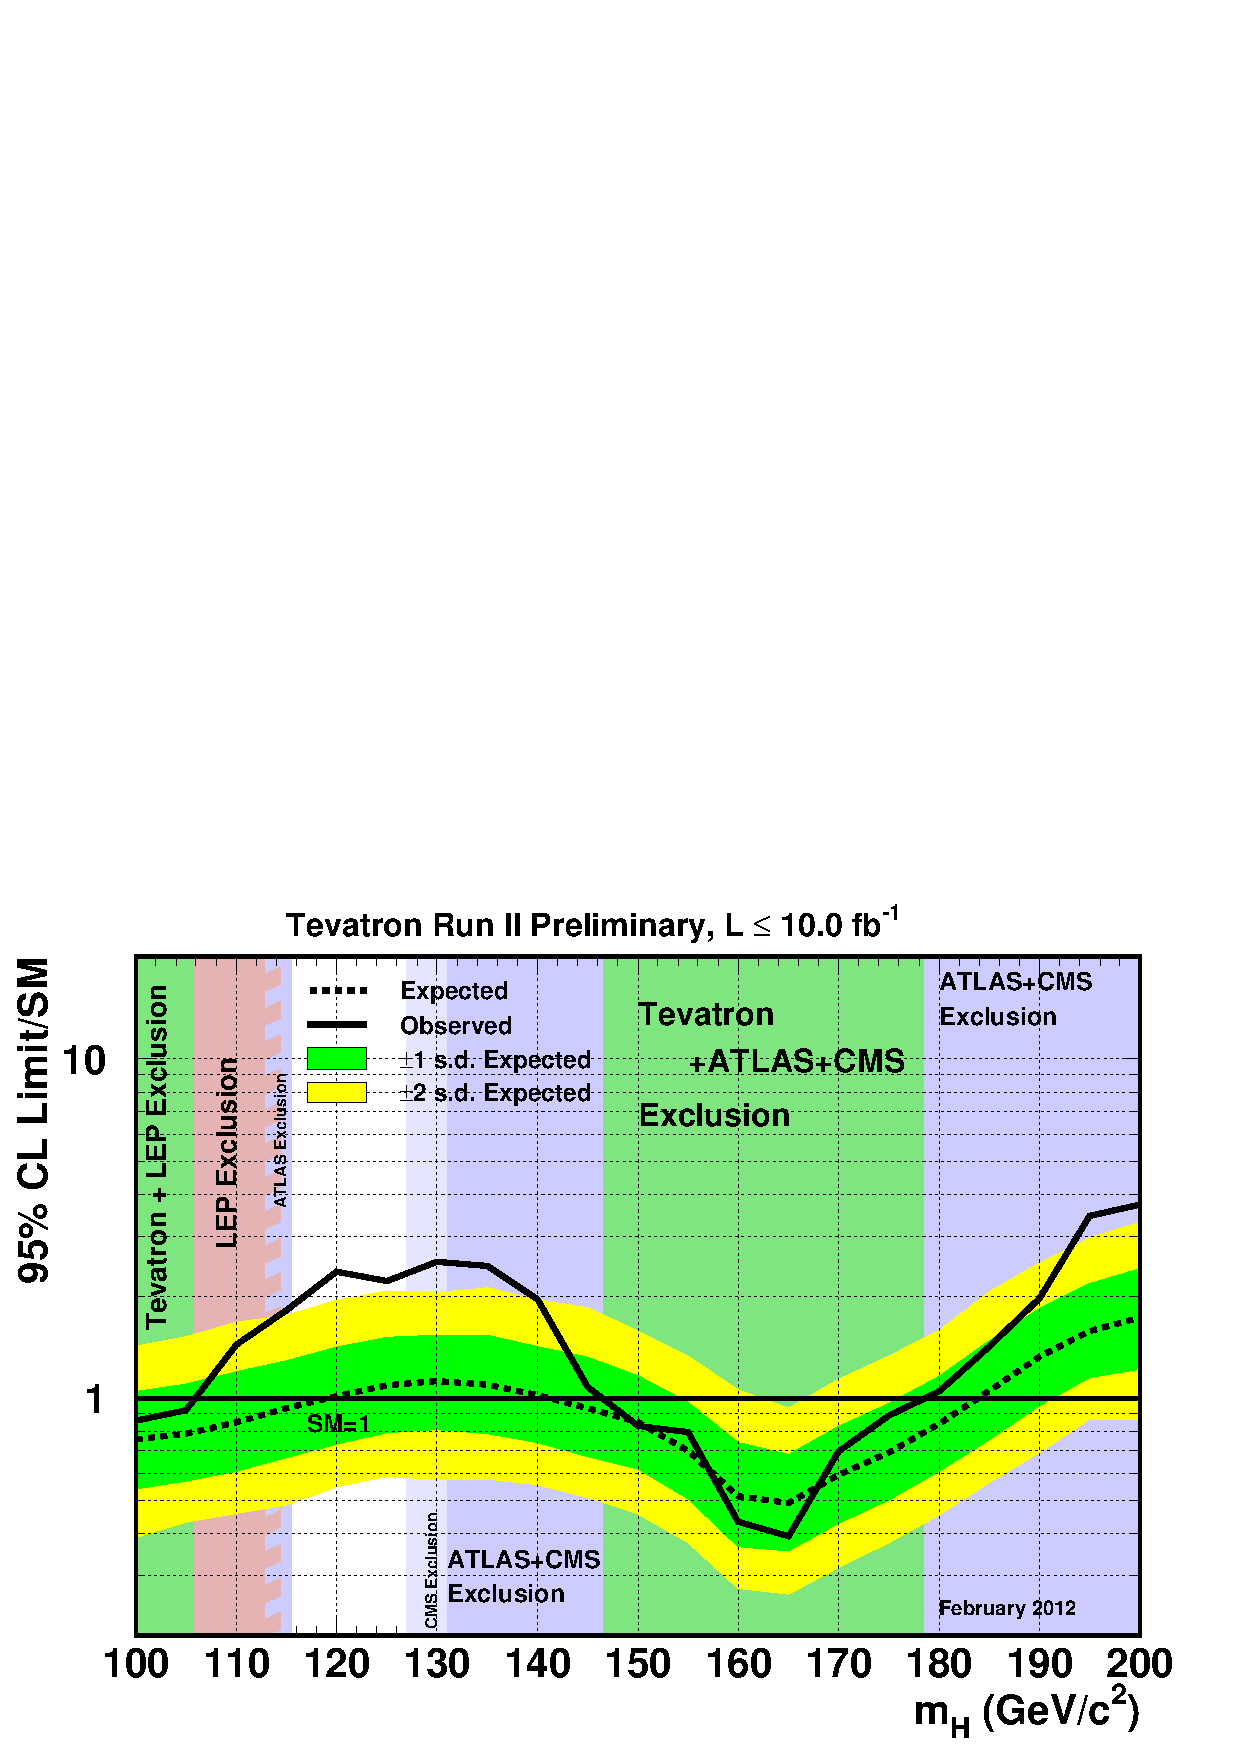
\includegraphics[width=0.4\textwidth]{plots/tev28febsmbayeslimits.pdf}}
%\centerline{\includegraphics[width=0.4\textwidth]{plots/cmshiggs.pdf}\includegraphics[width=0.4\textwidth]{plots/atlashiggs.pdf}}
\caption{
  Higgs exclusion as a function of mass at LEP\cite{PDGREVIEW}.
}
\label{fig:lepexclusion}
\end{center}
\end{figure}

The Tevatron was a $p\overline{p}$ collider located at Fermilab National Laboratory, just west of Chicago, IL. 
It operated at a center of mass energy $\sqrt{s} = 1.96$ TeV.
At the Tevatron a number of different channels contributed to the sensitivity of the Higgs search, the more notable being $H \rightarrow b\overline{b}$ at low Higgs mass, and $H \rightarrow W^{+}W^{-}$ at higher mass\cite{TEVHIGGS}.
The combined Tevatron Higgs exclusion can be seen in Figure \ref{fig:tevexclusion}.
The Tevatron has two exclusion regions, the first is $100 < m_{H} < 106$ GeV, and the second being $147 < m_{H} < 179$ GeV.
Further, the result contains an excess of events above background expectations in the range $115 < m_{H} < 135$ GeV with a global significance of approximately 2.2 standard deviations.
\begin{figure}[htpb]
\centerline{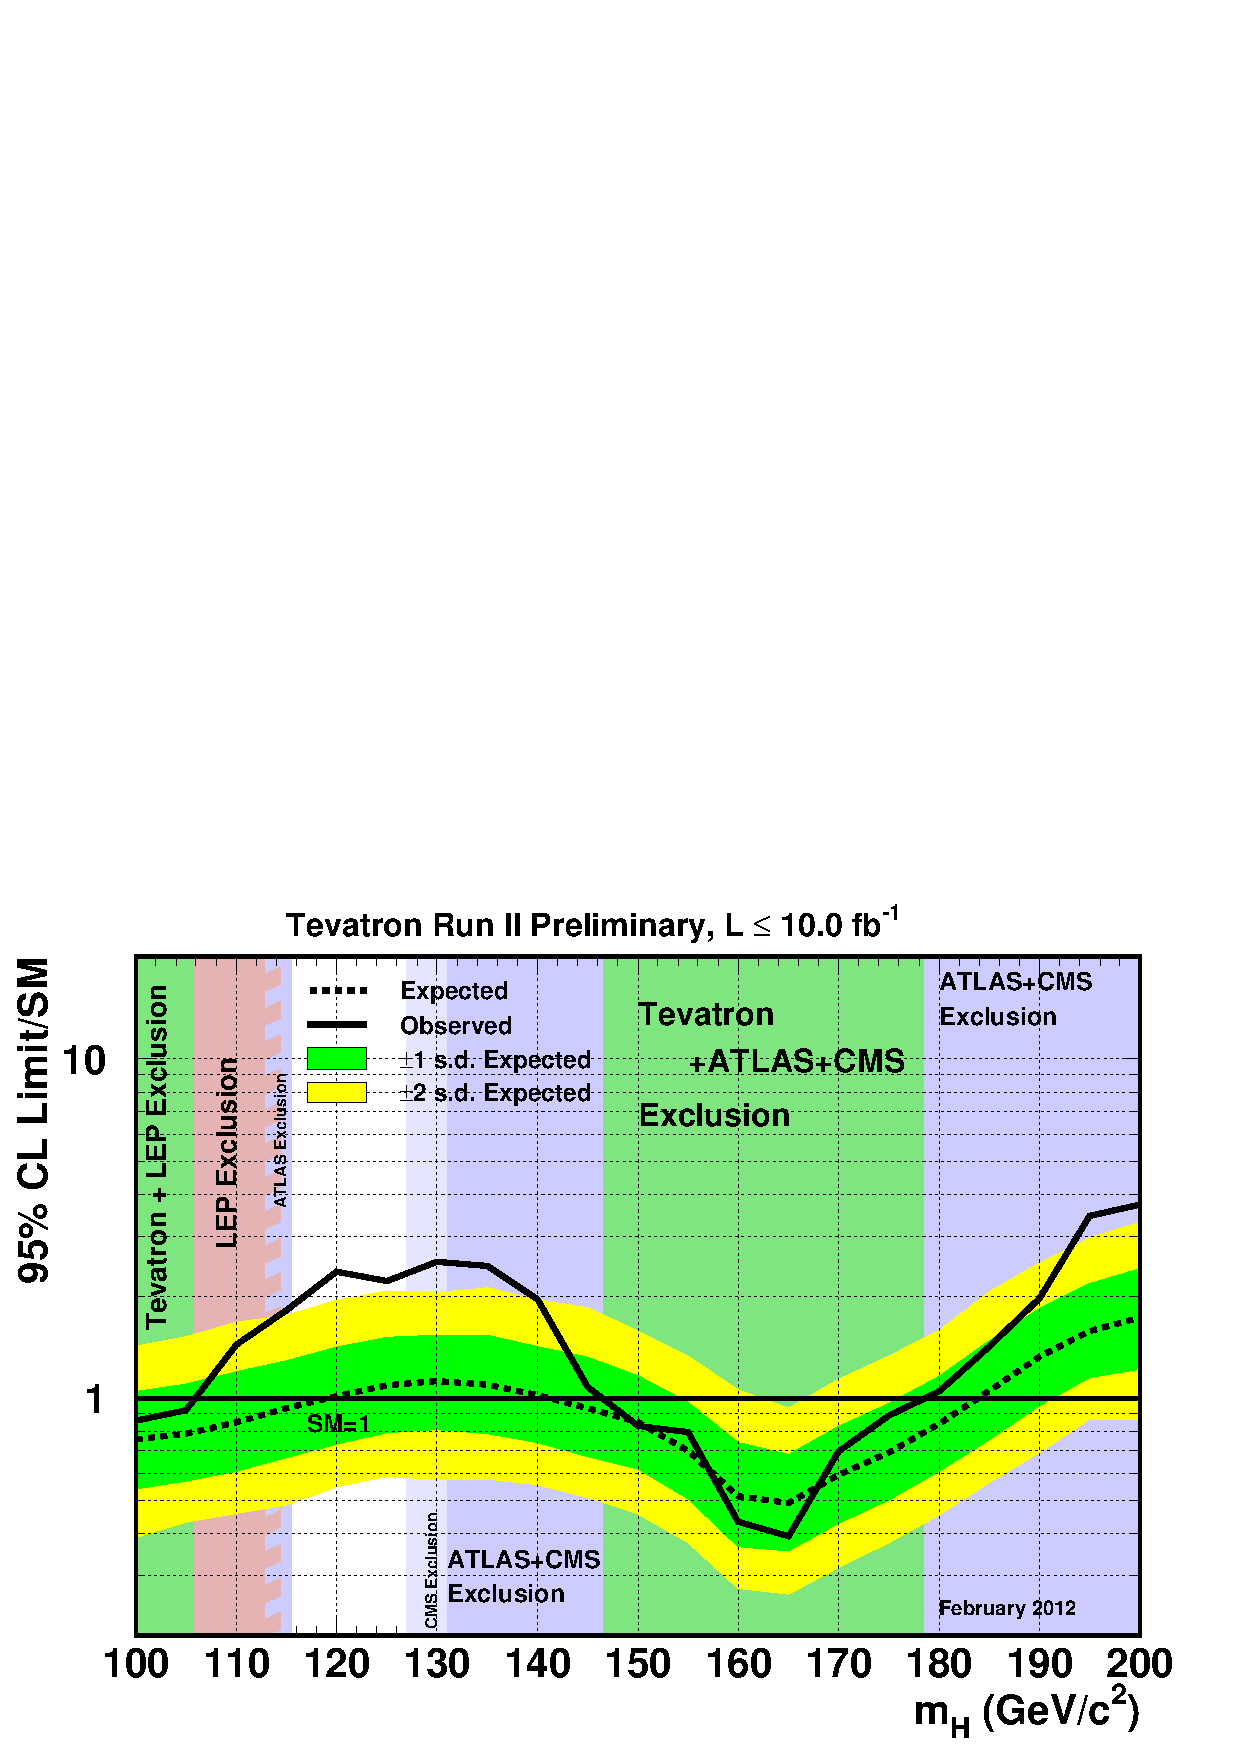
\includegraphics[width=0.85\textwidth]{plots/tev28febsmbayeslimits.pdf}}
\caption{Higgs exclusion at Tevatron\cite{TEVHIGGS}.}
\label{fig:tevexclusion}
\end{figure}

Due to the higher momentum protons at the LHC, it is much more probable that two gluons will interact to produce a Higgs boson, thus the dominant production mechanism is gluon gluon fusion.
Gluon gluon fusion is the process by which two gluons produce a Higgs boson through a fermion loop, shown in the left hand side of Figure \ref{fig:smproduction}\cite{PDGREVIEW}. 
A smaller, but still significant production mechanism at the LHC is vector boson fusion, as shown in the right hand side of Figure \ref{fig:smproduction}.
In vector boson fusion, two incoming quarks each radiate a gauge boson which then fuse, producing a Higgs boson.
The production cross sections as a function of the Higgs mass can be seen in the left hand side of Figure \ref{fig:higgsproduction}.
One can see that the production rate of vector boson fusion is approximately one tenth that of gluon fusion. 
Due to the lack of color change in this process it yields the unique signature of having low central jet activity while having two boosted jets in either hemisphere of the detector.
This unique signature makes it possible to identify and remove events of many background processes that would otherwise make the measurement more difficult.
\begin{figure}
\begin{center}
\ggfusion
\begin{fmffile}{vectorbosonfusion} 	%one.mf will be created for this feynman diagram  
\fmfframe(0,10)(0,10){ 	%Sets dimension of Diagram
\begin{fmfgraph*}(110,102) %Sets size of Diagram
\fmftop{iq1,oq1}
\fmfbottom{iq2,oq2}
\fmfright{H}    %Sets there to be 2  outputs
\fmflabel{$q$}{iq1}
\fmflabel{$q$}{oq1}
\fmflabel{$q^{\prime}$}{iq2}
\fmflabel{$q^{\prime}$}{oq2}
\fmflabel{$H$}{H}
\fmf{fermion,tension=2}{iq1,v1,oq1} %Connects the sources with a vertex.
\fmf{fermion,tension=2}{iq2,v2,oq2} %Connects the sources with a vertex.
\fmf{photon,label=$W^{\pm}/Z$}{v1,v3}
\fmf{photon,label=$W^{\mp}/Z$}{v2,v3}
\fmf{dashes,tension=.1}{H,v3}
\end{fmfgraph*}
}
\end{fmffile}
\caption{
  Feynman diagrams of prominent SM Higgs production mechanisms at the LHC. Gluon fusion (left) and vector boson fusion (right).
}
\label{fig:smproduction}
\end{center}
\end{figure}

Both the Compact Muon Solenoid (CMS) and A Large Toroidal LHC Apparatus (ATLAS) have performed Higgs searches in a broad number of channels.
One can see from Figure \ref{fig:higgsproduction} that in the low Higgs mass regime the branching ratio of $H\rightarrow b\overline{b}$ dominates, however due to the high cross section of QCD multi-jet events this is a very difficult channel at the LHC.
Rather than $H \rightarrow b\overline{b}$ contributing most to the sensitivity at low Higgs mass, it is in the $H\rightarrow\gamma\gamma$ channel that the majority of the sensitivity lies.
The sensitivity of the $H\rightarrow\gamma\gamma$ channel is due primarily to the low number of background processes that are associated with it.
In the high mass region as the branching ratios indicate, the $H\rightarrow WW$ and $H\rightarrow ZZ$ channels are the dominant search channels.
The combined Higgs exclusion for the CMS detector can be seen in Figure \ref{fig:lhcexclusion}.
Between CMS and ATLAS the exclusion range for the Higgs is found to be $127 < m_{H} < 600$ GeV.
Both experiments see a similar excess in the region around $124$ GeV, CMS with a local significance of $3.1\sigma$ and a global significance of $2.1\sigma$.
With more than one indication of an excess of signal, it is an exciting time in High Energy Physics as a breakthrough may be right around the corner.
\begin{figure}[htpb]
\begin{center}
%\includegraphics[width=0.4\textwidth]{plots/tevhiggsproduction.png}
\centerline{\includegraphics[width=0.51\textwidth]{plots/lhchiggsproduction.png}\includegraphics[width=0.38\textwidth]{plots/higgsbr.jpg}}
\caption{Standard Model Higgs boson production cross sections at the LHC energy scale\cite{HIGGS_PRODUCTION}.}
\label{fig:higgsproduction}
\end{center}
\end{figure}

\begin{figure}[htpb]
\label{fig:lhcexclusion}
\begin{center}
\centerline{\includegraphics[width=0.60\textwidth]{plots/cmshiggs.pdf}}
%\centerline{\includegraphics[width=0.63\textwidth]{plots/atlashiggs.pdf}}
\caption{Higgs exclusion as a function of mass at CMS\cite{CMSHIGGS}.}
\label{fig:lhcexclusion}
\end{center}
\end{figure}

\subsection{The Higgs Search in the Minimal Supersymmetric Standard Model}
If the excess of signal seen at the Tevatron and the LHC does indeed yield a discovery of the Higgs boson at a mass around $124$ GeV, it does not signify the end of the story for the Higgs boson.
As discussed in Section \ref{sec:mssm}, the MSSM will likely induce an enhanced coupling between the Higgs boson and bottom quarks and tau leptons as per Equation \ref{eqn:mssmcouplings}.
Indeed at a mass of $124$ GeV, this puts the Higgs at a mass in which the branching ratio to tau leptons is favorable, and in the case of the MSSM the Higgs will decay to tau leptons approximately $10\%$ of the time, and to bottom quarks approximately $90\%$ of the time.
The difficulty in performing an analysis involving bottom quarks in a hadron collider environment such as the LHC makes the search for the Higgs in the channel $H\rightarrow\tau^{+}\tau^{-}$ all the more attractive.

In the MSSM, the dominant Higgs production mechanisms are slightly different than the SM.
In particular, the cross section and branching ratio to tau leptons for the heavy CP-even ($H$) and CP-odd ($A^{0}$) Higgs bosons are considered.
While the gluon fusion production mechanism remains dominant as in the SM, due to the enhanced coupling to the bottom quark the vector boson fusion mechanism is supplanted by the associated production with bottom quarks as shown in the right hand side of Figure \ref{fig:mssmproduction}.
Not only does the associated production mechanism rate increase, but at high $tan\beta$ this mechanism can have a greater cross section than that of gluon fusion.
The production cross section times branching ratio to two tau leptons ($\sigma\times BR(\tau\tau)$) for the MSSM as compared to the SM can be seen in the left portion of Figure \ref{fig:mssmcrosssections}, while the enhanced branching ratio to the tau lepton can be seen on the right.
One can see that the branching ratio to tau leptons remains constant over a much larger mass range than in the SM.
This enhancement comes at the expense of a decreased branching ratio to $W$ and $Z$ bosons, making the search in the $H\rightarrow\tau\tau$ channel very important.
\begin{figure}
\begin{center}
\ggfusion
\begin{fmffile}{associatedprod} 	%one.mf will be created for this feynman diagram  
\fmfframe(1,7)(1,7){ 	%Sets dimension of Diagram
\begin{fmfgraph*}(110,102) %Sets size of Diagram
\fmftop{g1,b1}
\fmfbottom{g2,b2}
\fmfright{H}    %Sets there to be 2  outputs
\fmflabel{$g$}{g1}
\fmflabel{$g$}{g2}
\fmflabel{$H$}{H}
\fmflabel{$b$}{b2}
\fmflabel{$\overline{b}$}{b1}
\fmf{gluon,tension=2}{g1,v1} %Connects the sources with a vertex.
\fmf{gluon,tension=2}{g2,v2} %Connects the sources with a vertex.
\fmf{fermion,tension=2}{b1,v1,v3,v2,b2} %Connects the sources with a vertex.
\fmf{dashes,tension=.1}{H,v3}
\end{fmfgraph*}
}
\end{fmffile}
\caption{
  Feynman diagrams of prominent MSSM Higgs production mechanisms at the LHC. Gluon fusion (left) and associated production with b quarks (right).
}
\label{fig:mssmproduction}
\end{center}
\end{figure}
\begin{figure}[htpb]
\begin{center}
\centerline{\includegraphics[width=0.45\textwidth]{plots/cross-sections.pdf}\includegraphics[width=0.45\textwidth]{plots/branching-ratios.pdf}}
\caption{
  On the left the Higgs production cross sections are compared between MSSM and SM mechanisms. The blue and red bands represent the range of the cross section between low $tan\beta = 5$ and high $tan\beta = 30$. On the right the branching ratio for $H\rightarrow\tau^{+}\tau^{-}$ is compared for various values of $tan\beta$ in the MSSM to the SM branching ratio}
\label{fig:mssmcrosssections}
\end{center}
\end{figure}


\section{The Tau Lepton}
The Tau lepton ($\tau$) is the heaviest of the three leptons with a mass of $1.87$ GeV. 
It also has the shortest lifetime, traveling a typical distance of $86$ $\mu$m before decaying.
This means that the tau lepton will decay before reaching any active detector element. 
As will be discussed in Section \ref{sec:tracker}, the charged particle tracking system used at CMS has very good spatial resolution and can reconstruct the displaced decay vertex of a tau lepton.
The tau lepton can decay leptonically to either an electron or a muon, along with two neutrinos.
More likely  however is that the tau will decay hadronically, producing a low multiplicity and collimated jet of mesons. 
The jet resulting from a tau lepton decay typically contains $\pi^{\pm}$ and $\pi^{0}$ mesons, along with a single neutrino which at high energies will be colinear with the jet.
When decaying hadronically the tau lepton often passes through an intermediate resonance (the $\rho$ meson for example), which can be seen in Table \ref{tab:taudecays} along with the branching ratios for the most common decay modes.

The properties of the tau lepton make it a difficult physics object to deal with at hadron colliders, for example when compared to the muon.
The first difficulty arises in that the tau decay always has an associated neutrino which interacts only weakly and cannot be directly detected.
The tau lepton decays hadronically approximately 65\% of the time which leads to the second difficulty. 
Hadron colliders typically have large QCD multi-jet activity, thus identifying a hadronic tau decay against other jets in an event can be difficult.
In order to accomplish this, the low multiplicity of a hadronic tau decay is leveraged. 
Further discrimination power can be achieved by checking for the compatibility of an intermediate resonance.
One can consider the implications of these difficulties in terms of the different final states that the $H\rightarrow\tau\tau$ channel will have.
The case where both taus decay leptonically would yield a much cleaner signal, but the branching ratio for this case is very small.
Additionally, in the case where both taus decay to the same flavor of lepton, the signal would be very difficult to distinguish from $Z\rightarrow ll$ events.
In contrast the branching ratio is significantly higher in the case that both taus decay hadronically, this however leads to very high QCD multi-jet backgrounds which will make the analysis more difficult.
One can find a satisfactory middle ground in the case where one tau decays leptonically and the other decays hadronically.
If the leptonic leg of the decay is an electron, the backgrounds from $Z\rightarrow ee$ are found to be a bit higher than the case of a muon. 
The higher backgrounds from $Z\rightarrow ee$ events is due to electrons having a higher mis-identification rate than muons.
Thus the search for the Higgs boson decaying to two tau leptons in which one tau decays to a muon and the other decays hadronically is a favored channel in that it optimizes the production rate and branching ratio while minimizing the backgrounds of the process.

\begin{table}[htpb]
  \begin{center}
    \caption{TAU LEPTON DECAY MODES}
    \label{tab:taudecays}
    \begin{tabular}{lccr}
      \toprule
      Final State & Resonance & Mass (MeV) & Branching Ratio \\
      \midrule
%      $e^{-}\nu_{\tau}\overline{\nu}_{e}$ & - & $0.5$ & $17.8\%$ \\
%      $\mu^{-}\nu_{\tau}\overline{\nu}_{\mu}$ & - & $105$ & $17.4\%$ \\
%      $\pi^{-}\nu_{\tau}$ & - & $135$ & $10.9\%$ \\
      $e^{-}\nu_{\tau}\overline{\nu}_{e}$      & -      & -      & $17.8\%$ \\
      $\mu^{-}\nu_{\tau}\overline{\nu}_{\mu}$  & -      & -      & $17.4\%$ \\
      $\pi^{-}\nu_{\tau}$                      & -      & -      & $10.9\%$ \\
      $\pi^{-}\pi^{0}\nu_{\tau}$               & $\rho$ & $770$  & $25.5\%$ \\
      $\pi^{-}\pi^{0}\pi^{0}\nu_{\tau}$        & $a1$   & $1260$ & $9.3\%$  \\
      $\pi^{-}\pi^{-}\pi^{+}\nu_{\tau}$        & $a1$   & $1260$ & $9.0\%$  \\
      $\pi^{-}\pi^{-}\pi^{+}\pi^{0}\nu_{\tau}$ & $a1$   & $1260$ & $4.5\%$  \\
      \bottomrule
    \end{tabular}
  \end{center}
\end{table}



\chapter{DETECTOR}
\label{chap:detector}
The Large Hadron Collider (LHC) is a proton-proton synchrotron located along the French/Swiss border near Geneva, Switzerland which utilizes the same accelerator tunnel that was originally built for LEP.
The collider operates by using superconducting magnets to steer opposing beams of protons around a 27 kilometer circumference. 
The protons are accelerated by means of radio-frequency resonating cavities.
The protons in the LHC have a maximum energy (design) of $7$ TeV in each direction, providing a center of mass collision energy ($\sqrt{s}$) of $14$ TeV.
The analysis presented in this text will focus on the data taken at the Compact Muon Solenoid experiment in 2011, during which time, the center of mass collision energy of the LHC was $7$ TeV.
A common figure of merit for the performance of an accelerator is the luminosity, which can be simply described as the number of particles per unit area per unit time.
The LHC design luminosity is $10^{34}$ \lumiunit, while during the 2011 data taking the peak luminosity reached approximately $5\times 10^{33}$ \lumiunit.
The LHC has four collision points located around its circumference, at these points the proton beams are confined and collided.
There is a detector situated around each of these collision points: The Compact Muon Solenoid (CMS), A Toroidal LHC Apparatus (ATLAS), LHC-B, and A Large Ion Collider Experiment (ALICE).

The analysis presented in this thesis was performed on the CMS detector, thus a brief description of the detector will be given.
The CMS detector is one of two general purpose detectors, the other being the ATLAS detector.
Being a general purpose detector, the CMS detector is designed to observe a wide range of physics processes. 
The CMS detector has a hermetic design such that it is capable of measuring nearly any and all particles that arise from the collisions with little acceptance loss.
A cartesian coordinate system is defined for the CMS detector as follows: the $z$ axis points along the beam pipe, the $y$ axis pointing up with respect to gravity, and the $x$ axis pointing towards the center of the LHC ring.
The CMS detector is designed in the shape of a cylinder, and as such a cylindrical coordinate system is also defined.
The $z$ axis of the cylindrical coordinate system is the same as the $z$ axis of the cartesian coordinate system.
The polar angle ($\theta$) is measured with respect to the $z$ axis with $\theta = 0$ being the positive $z$ axis, and $\theta = \pi$ being the negative $z$ axis.
The azimuthal angle ($\phi$) is measured with respect to the $x$-$y$ plane, $\phi = 0$ is the positive $x$ axis and $\phi = \frac{\pi}{2}$ is the positive $y$ axis.
Rather than the polar angle, it is often more useful to consider the pseudorapidity, $\eta = -ln\left[tan\left(\frac{\theta}{2}\right)\right]$, which for high energy particles approximates the rapidity $y = \onehalf ln\frac{E+p_{T}}{E-p_{T}}$. 
Pseudorapidity is useful in that it is related to the relativistic boost of a particle.
To accomplish the task of observing and measuring the properties of different processes and particles the CMS detector has multiple subsystems dedicated to different tasks.
The inner-most sub system is a tracking device that measures the trajectory of charged particles.
Just outside the tracking system are two calorimeters, first the electric calorimeter (ECAL) which measures the energy of photons and electrons. 
The calorimeter system is completed by the hadronic calorimeter (HCAL) which measures the energy of jets of hadrons and is situated just outside the ECAL.
A superconducting solenoid magnet provides a powerful magnetic field which bends the trajectory of charged particles allowing the measurement of a charged particle's momentum and charge.
The solenoid magnet encloses the tracking system and calorimeter systems.
Finally outside the solenoid is the muon system which measures the trajectory of particles that escape the calorimeters.
Since the calorimeters are designed to completely absorb the energy of all other particles, with limited exceptions the only particles that reach the outer muon system are muons.
A labeled schematic of the CMS detector and its subsystems is given in Figure \ref{fig:cmsdetector}.
\begin{figure}[ht]
\centering
%\begin{center}
\includegraphics[width=0.9\textwidth]{plots/cmsdetector.pdf}
\caption{Schematic of the CMS detector\cite{CMS_DETECTOR}.}
\label{fig:cmsdetector}
%\end{center}
\end{figure}
\section{The Large Hadron Collider}
\label{sec:lhc}
Protons are delivered to the LHC by means of multiple intermediate accelerators: the Lineac2, the Proton Synchrotron Booster, the Proton Synchrotron (PS), and the Super Protron Synchrotron (SPS).
The PS was the first circular particle accelerator built at CERN in the late 1950s. 
In its current implementation the PS takes protons that originate in the Lineac2 linear accelerator at $50$ MeV that are then accelerated in the Proton Synchrotron Booster to $1.4$ GeV.
The protons are fed from the PS to the SPS which was commissioned in 1976 and has served to accelerate protons, antiprotons, electrons and positrons for various accelerators over its history.
Most notably the SPS accelerator provided the proton-antiproton beams that were used for the UA1 and UA2 experiments that accomplished the discovery of the $W$ and $Z$ bosons.
The SPS later provided the $e^{+}e^{-}$ beams that were used for LEP.
The two proton beams for the LHC are accelerated to their injection energy of $450$ GeV in the SPS at which point the radio-frequency resonating cavities of the LHC accelerate the beams to their collision energies.
A diagram of the CERN accelerator complex is shown in Figure \ref{fig:lhc}
\begin{figure*}[htpb]
\begin{center}
\includegraphics[width=0.85\textwidth]{plots/lhc.png}
\caption{Schematic of the CERN accelerator complex including intermediate accelerators that deliver the proton beams used in the LHC.}
\label{fig:lhc}
\end{center}
\end{figure*}

The proton is a composite particle, which in addition to having three ``valence'' quarks contains more sub-structure in the form of virtual quarks and gluons. 
In Section \ref{sec:qcd} it was shown that gluons interact with both themselves and quarks, thus the gluons that hold the proton together are responsible for producing quark-antiquark pairs which exist inside the proton.
The individual components, or partons, of the proton will each carry some fraction of the total momentum of the proton which is given by the parton distribution function (pdf) and is dependent on the energy of the proton.
In a hadron collision it is in fact the partons that produce the interaction rather that the proton itself.
The pdfs give the probability of finding a particular parton with longitudinal momentum fraction $x$ at a given momentum $Q$. 
Two example pdfs are shown in Figure \ref{fig:pdf}, one for low $Q$ and one for high $Q$.
Upon examination of Figure \ref{fig:pdf} one can see that as the energy of the proton increases, so too does the fraction of the momentum carried by the gluons.
At the energy of the LHC the pdf of the proton is dominated by gluons. 
%In comparison to the LHC, at the energy of the Tevatron the quarks carry a larger fraction of the momentum.
%For this reason colliding protons at the LHC would be somewhat equivalent to colliding protons and antiprotons, as it is more often that the interactions observed are provided by interacting gluons.
At the energy of the LHC, the dominance of the gluon in the pdf means that the majority of interactions are due to two gluons. 
Thus, there is little advantage in colliding protons and anti-protons.
This combined with the fact that antiprotons are difficult to produce and store leads to the conclusion that a proton-proton collider at the LHC energy scale is the logical choice.
\begin{figure*}[htpb]
\begin{center}
\includegraphics[width=0.85\textwidth]{plots/pdf.png}
\caption{Distributions of $x$ times the parton fraction $f(x)$ for the constituents of the proton at $Q^{2} = 10$ GeV$^{2}$ (left) and $Q^{2} = 10,000$ GeV$^{2}$\cite{PDGREVIEW}.}
\label{fig:pdf}
\end{center}
\end{figure*}


The collision of two protons rather than protons and antiprotons, while negating the difficulty of producing and storing antiprotons, leads to other difficulties.
The colliding particles now have the same charge and as such cannot share the same steering magnets. 
Two separate beam pipes and magnet systems must be used to steer the protons around the LHC ring in different directions.
An additional difficulty at the LHC is the energy at which the protons must be collided in order to probe new physics.
In order to steer the proton beams at an energy of $7$ TeV, dipole magnets are used which must be capable of providing greater than $8$ T magnetic fields.
The superconducting dipole magnets are made of \ce{NbTi} cables that are cooled to superfluid temperatures of $\sim2$ K.
An important aspect of superconducting magnets is quenching, or the process by which the magnet returns to a normal resistive state.
Quenching can occur due to heat dissipation inside the magnet.
A quench can be induced by increasing the current of the magnet, and as a result heat dissipation in the magnet will raise the temperature beyond the critical temperature of the material.
Upon re-energizing the magnet, a greater field can be achieved before a quench occurs, this process is referred to as a training quench.
Due to the number of training quenches required to bend the proton beams at their full $7$ TeV energy, it was decided to operate the accelerator with proton beams of $3.5$ TeV during the 2010 and 2011 data collection periods.
The data collection period of 2012 will see the beam energy increase to $8$ TeV, with the beam increasing to the design energy some time after the maintenance period of 2013-2014.

The magnitude of the Higgs signal to that of common QCD multi-jet events was shown in Section \ref{sec:history}, and similar situations exist for other new physics signals.
%The relative production rates of new physics and the QCD multi-jet processes is what drives the desire to operate the LHC at very high instantaneous luminosities.
In order to probe these rare processes a large number of interactions must be produced in order to collect statistically significant samples, thus the drive for very high integrated luminosities is demonstrated.
During the 2010 data collection period a total integrated luminosity of $36$ pb$^{-1}$ was collected, while during the 2011 data collection period a total integrated luminosity of $4.6$ fb$^{-1}$ was collected.
The integrated luminosity of the 2012 data collection period is projected to be in the range of $15$-$20$ fb$^{-1}$.
The schedule for the increase in luminosity at the LHC is enumerated in Table \ref{tab:lhcluminosity}.
In order to achieve a high luminosity, protons are grouped into high density ``bunches'' made up of multiple protons that are accelerated around the LHC ring. 
By bunching the protons together the probability of two protons having a hard scatter, or collision, is increased.
The luminosity can then be increased by increasing the number of protons in each bunch, thus increasing the number of interacting protons per collision, $N_{1}$ and $N_{2}$ for either beam.
The luminosity can further be increased by placing a larger number of bunches ($n$) in the LHC ring leading to a higher collision rate.
Finally the cross sectional area ($A$) of the beam is minimized at the collision points to maximize the probability of a collision. 
These three factors can be seen in the following equation that gives the instantaneous luminosity,
\begin{equation}
\Lagr = fn\frac{N_{1}N_{2}}{A}.
\end{equation}
A side effect of increasing the luminosity in this way is that while increasing the probability of an interesting collision, the probability of ``uninteresting'' collisions is also increased.
In fact it is common for multiple interactions to occur in the same bunch, up to $\sim 35$ in some cases for the 2011 data collection.
This presents a challenge to an analysis performed at a hadron collider in that each event contains an effective ``pile-up'' of multiple events that must be taken into account when searching for new physics.

\begin{table}[htpb]
\begin{center}
\caption{LHC LUMINOSITY INCREASE SCHEDULE}
\begin{tabular}{lc}
\toprule
Year & Integrated Luminosity [fb$^{-1}$] \\
\midrule
2010 & $0.036$ \\
2011 & $4.6$ \\
2012 & $15$-$20$(projected) \\
\bottomrule
\end{tabular}
\label{tab:lhcluminosity}
\end{center}
\end{table}
% magnets
% proton-proton
% luminosity


\section{Superconducting Magnet}
\label{sec:magnet}
As the name the Compact Muon Solenoid implies the superconducting solenoid magnet is a central feature of the CMS detector.
The magnetic field is necessary to measure the momentum of charged particles produced in the proton-proton collisions.
As a charged particle travels through a magnetic field the radius of curvature for the charged particle is given by
\begin{equation}
r = {p_{\perp}\over|q|B},
\end{equation}
where $p_{\perp}$ is the component of the particle's momentum that is transverse to the direction of the magnetic field, $q$ is the charge of the particle, and B is the strength of the magnetic field.
As the radius of curvature is proportional to $p_{\perp}$, it becomes clear that to measure high momentum particles a very large magnetic field is required.
In addition to the requirement for the magnetic field to be large, it is also important that magnetic field be homogeneous in the volume of the detector to reduce systematic errors that result from a non-uniform field.

In order to provide a homogeneous magnetic field the CMS solenoid is required to be physically large, encapsulating the tracking system and calorimeters.
It has a radial bore of 6.3 meters, a length of 12.9 meters, and a weight of 220 tons.
The solenoid is made of four layers of wire with a total of 2168 turns carrying a nominal current of 19.14 kA.
A second momentum measurement is applied to muons that are detected in the muon system surrounding the solenoid, for this reason the muon system is interspersed throughout the iron return yoke.
The return yoke has the effect of minimizing the fringe field outside the solenoid, providing a homogeneous field throughout the muon system. %FIXME return yoke necessary

\section{Charged Particle Tracking System}
\label{sec:tracker}
The charged particle tracking system is the sub-detector that lies closest to the beam pipe.
Its purpose is to measure the the trajectories of charged particles that emerge from the collisions.
The trajectories are then used to determine the momentum and charge of the charged particles.
In order to measure the trajectories several layers of silicon detectors are used, as charged particles traverse these layers they create electronic signals in the silicon.
Each of these signals, often referred to as ``hits'', correspond to the position of a charged particle as it travels through the detector.
The hits that are measured in the tracking system are fit to a helix producing the trajectories that are used to measure the charge and momentum.
For high momentum tracks the tracking system provides very good resolution for the transverse momentum of approximately $1-2\%$ in the barrel region, while in the endcap region ($|\eta| > \sim1.5$) the resolution degrades as can be seen in Figure \ref{fig:trackerptres}.
\begin{figure}[htpb]
\begin{center}
\includegraphics[width=0.85\textwidth]{plots/trackerptres.pdf}
\caption{Transverse momentum resolution of the CMS tracking system as a function of pseudo-rapidity ($\eta$) for muons with $p_{T} = 1$, $10$, and $100$ GeV\cite{CMS_DETECTOR}.}
\label{fig:trackerptres}
\end{center}
\end{figure}

The tracking system is designed to have the capacity of measuring secondary decay vertices, for example, arising from the decay of bottom quarks and tau leptons.
Bottom quarks and tau leptons have relatively long life times, as such they travel a non-negligible distance before decaying, giving rise to secondary decay vertices.
In order to measure secondary decay vertices, the tracking system is constructed using two technologies, an inner tracking system consisting of silicon pixel detectors and an outer tracking system of silicon strips.
The inner layer of the pixel tracking system is placed at a radius of $4.4$ cm in order to be as close as possible to the interaction point.
This pixel tracking system is made up of three layers in the barrel and two layers in the endcaps.
Outside the pixel tracking system is the silicon strip tracking system consisting of ten layers of silicon strips in the barrel region and 12 layers in the endcaps. 
A schematic of the CMS tracking system can be seen in Figure \ref{fig:trackerlayout}.
The transverse impact parameter ($d_{0}$) resolution of the tracking system gives an indication of the performance one can expect for the secondary decay vertex reconstruction, for high momentum tracks the resolution is approximately $10$ \micrometer as can be seen in Figure \ref{fig:trackerd0res}. %FIXME micrometer
For lower momentum tracks the resolution of $d_{0}$ degrades due to multiple scattering of the particle in the tracker material.
\begin{figure}[htpb]
\begin{center}
\includegraphics[width=0.85\textwidth]{plots/trackerlayout.png}
\caption{Schematic of the CMS inner tracking system\cite{CMS_DETECTOR}. The barrel tracker is divided into the Tracker Inner Barrel (TIB) and Tracker Outer Barrel (TOB). The endcap tracker is divided into the Tracker End Cap (TEC) and Tracker Inner Disks (TID).}
\label{fig:trackerlayout}
\end{center}
\end{figure}

\begin{figure}[htpb]
\begin{center}
\includegraphics[width=0.85\textwidth]{plots/trackerd0res.pdf}
\caption{Transverse impact parameter resolution of the CMS tracking system a function of pseudo-rapidity ($\eta$) for muons with $p_{T} = 1$, $10$, and $100$ GeV\cite{CMS_DETECTOR}.}
\label{fig:trackerd0res}
\end{center}
\end{figure}

Both the inner and outer tracking systems consist entirely of silicon, which operate by doping the silicon and thus creating a diode. % FIXME reword?
A reverse bias is then applied to the silicon to deplete the region, so that when a charged particle passes through the silicon a small ionization current is induced which can then be measured.
The most common method of forming this type of silicon diode is to create a p-n junction, however to ensure radiation hardness the layering in the tracking system silicon is more complicated\cite{CMS_DETECTOR}. %FIXME involves creating
In order to achieve high resolution track measurements suitable for the measurement of secondary decay vertices and particle impact parameters, the pixels in the inner layers are electronically isolated and constructed in sizes of $100$x$150$ \micrometer.
The tracking system was designed such that the occupancy would be less than or equal to 1\% at the design luminosity, and as such the outer tracking system does not need to be as finely divided as the inner pixel system.
The outer tracking system is constructed of silicon strips providing single point resolution between $23$ to $52$ \micrometer in both $r$-$\phi$ and $z$ directions.

Tracks are reconstructed from the reconstructed hits in the tracker by means of the Combinatorial Track Finder (CTF) algorithm\cite{TRACKRECO}.
The CTF begins by first locating pairs of reconstructed hits in the inner pixel detector that are compatible with the interaction region.
The track finding then uses a Kalman filtering method to combine the seeded parameters with nearby reconstructed hits.
During each step of the finding algorithm each track is assigned a quality, ambiguities that arise from two tracks are resolved by rejecting the track that is of lesser quality.
Once the track finding method is complete each track undergoes two least squares fitting procedures, the first is an inside-out fit that serves to remove any approximations or biases that arise from the seeding or finding algorithms.
The second fit is an outside-in fit that serves to smooth the final track.
The final track finding procedure is performed iteratively to improve the efficiency of the track finding process, the CTF is repeated three to four times.
After each iteration of the CTF a set of filters is applied setting aside high quality tracks and removing their reconstructed hits from the next iteration.
The iterative procedure has been shown to increase the track finding efficiency by approximately $5\%$ while keeping mis-identification rates low.
Further, the iterative procedure also allows for the reconstruction of low momentum tracks that would otherwise not be reconstructed with a single CTF.

\section{Electromagnetic Calorimeter}
\label{sec:ecal}
The electromagnetic calorimeter (ECAL) was designed with the specification of measuring the energy of particles that interact electromagnetically with a very high precision. 
The search for the Higgs boson in the channel $H\rightarrow\gamma\gamma$ was a driving factor in the design of the ECAL.
The ECAL is a hermetic, homogeneous detector constructed of scintillating lead tungstate (\ce{PbWO4}) crystals, 61200 in the barrel region, and 7324 in each of the endcaps.
Particles that interact electromagnetically, primarily electrons and photons, will cause electromagnetic showers in the ECAL material.
An electromagnetic shower is a process in which electrons and photons are created, via pair-production or bremsstrahlung respectively.
The ultimate conclusion of an electromagnetic shower is a collection of scintillation photons that are measured by photo multipliers which read out the signal of each crystal. %FIXME diodes?
The energy of the particle inducing the shower can be inferred from the number of photons that are collected.

To reliably measure the energy of an incident electron or photon, the total energy of the particle must be absorbed by the calorimeter, and thus a crystal must be capable of capturing the entire shower of a particle longitudinally.
The ability of the crystal to confine an electromagnetic shower is dependent on the depth of the crystal, the density of the crystal, and the radiation length of an electromagnetic shower in the material.
The radiation length ($X_{0}$) is a unit of measurement defined by the mean distance that an electron must travel before its energy is reduced by $(1-{1\over e})$.
These criteria were the driving choice in the decision to use \ce{PbWO4} crystals as this material is very dense, leading to maximal shower capture while maintaining a compact size.
The crystals used have a density of $8.28$ g/cm$^{3}$ and a length of $230$ mm resulting in a total radiation length of $25.8 X_{0}$
The Moliere radius is the lateral distance in which 90\% of an electromagnetic shower is contained. for \ce{PbWO4} this radius is $22$ mm. 
The inner facing cross section of the ecal crystals is $22\times22$ mm, such that if an incident particle were to hit the center of a crystal 90\% of the particle's energy would be contained in a single crystal.

% Transparency? FIXME

Below energies of $500$ GeV the energy resolution of the ECAL can be parameterized as a function of energy,
\begin{equation}
\label{eq:ecalresolution}
\left({\sigma \over E}\right)^{2} = \left({S \over \sqrt{E}}\right)^{2} + \left({N \over E}\right)^{2} + C^{2},
\end{equation}
where $S$ is the stochastic noise term, $N$ is the noise term, and $C$ is a constant.
The resolution of the ECAL as a function of energy was determined in 2004 by fitting the measured energy to Equation \ref{eq:ecalresolution} in a test beam of electrons with energies ranging from $20$ GeV to $250$ GeV, the results of the fit can be seen in Figure \ref{fig:ecalres}.
For energies above $20$ GeV the energy resolution of the ECAL is better than $1\%$\cite{CMS_DETECTOR}.
\begin{figure}[htpb]
\begin{center}
\includegraphics[width=0.85\textwidth]{plots/ecalres.png}
\caption{The CMS detector electromagnetic calorimeter energy resolution as a function of electron energy\cite{CMS_DETECTOR}.}
\label{fig:ecalres}
\end{center}
\end{figure}

\section{Hadronic Calorimeter}
\label{sec:hcal}
The hadronic calorimeter (HCAL) is designed to measure the energy of hadrons while providing good shower containment and hermicity.
The HCAL surrounds the ECAL and is inside the solenoid, with the exception of the hadronic outer (HO) detector which is placed just outside the solenoid.
The purpose of the HO is to catch any hadronic showers which are not fully contained within the bulk of the HCAL.
A schematic of the HCAL subsystem layout is shown in Figure \ref{fig:hcallayout}.
The HCAL is a sampling calorimeter in that it utilizes scintillating plastic tiles with embedded wavelength-shifting fibers (WLS), interspersed between brass absorber plates.
A hadron traveling through the HCAL will interact with the brass absorber producing a hadronic shower which produces photons as the particles in the shower pass through the scintillating tiles.
The photons captured in the tiles are then carried via the WLS to the hybrid photodiode based readout system.
%As the HCAL is a sampling calorimeter the radial profile of the hadronic shower can be measured by using each of the tiles separately giving an additional parameter to the measurement of the deposited energy.
\begin{figure}[htpb]
\begin{center}
\includegraphics[width=0.9\textwidth]{plots/hcallayout.png}
\caption{Schematic of the CMS hadronic calorimeter subsystem\cite{CMS_DETECTOR}.}
\label{fig:hcallayout}
\end{center}
\end{figure}

A forward calorimeter (HF) is used in addition to the HCAL barrel, endcaps, and HO. 
The HF spans the region from $\pm3.0$ to $\pm5.0$ in $\eta$, and is designed to measure the hadronic energy deposited in the congested high $\eta$ region.
Not only does the HF provide the ability to measure hadronic energy in the high $\eta$ regions, but also provides a method to measure the luminosity delivered to the CMS detector.
The HF is a Cherenkov detector with quartz fibers, running parallel to the beam line,  installed into grooves situated inside a steel absorber.
Hadronic showers that originate in the steel absorber will contain neutral and charged particles that will produce Cherenkov light if their energy is above a certain threshold.
The Cherenkov light is then measured to reconstruct the energy deposited in the calorimeter.
The quartz fibers used have two lengths where one length is shorter than the other, providing a means of separating electrons and photons from hadrons.
This is possible as showers produced from incident electrons and photons will deposit their energy very quickly and not travel as far as showers produced from incident hadrons.

The jet $E_{T}$ resolution as a function of transverse energy is shown in Figure \ref{fig:jetres}. The $E_{T}$ resolution is better than $20\%$ for jets with $E_{T} > 50$ GeV, and drops to $10\%$ for jets with $E_{T} > 300$ GeV.
\begin{figure}[htpb]
\begin{center}
\includegraphics[width=0.85\textwidth]{plots/jetres.pdf}
\caption{Jet energy resolution for the HCAL in the barrel, endcap and forward regions\cite{CMS_DETECTOR}.}
\label{fig:jetres}
\end{center}
\end{figure}

\section{Muon System}
\label{sec:muonsystem}
The detection of muons is a powerful tool at hadron colliders because they leave a unique signal in the detector.
The signal is unique for a couple of reasons:
\begin{itemize}
\item A muon is charged so a muon's momentum can be measured via its trajectory.
\item A muon is a minimum ionizing particle so it will be one of the few particles that does not leave much energy in the calorimeter systems.
\end{itemize}
The muon system for the CMS detector is situated in the iron return yoke of the solenoid. 
Although the components of the muon system are different than that of the tracking system, it reconstructs charged particle tracks in a similar manner.
Being situated outside of the calorimeters and solenoid, all other particles that would otherwise interact with the muon system are stopped before reaching it.
A muon can be identified by matching a track in the inner tracking system to a track in the muon system.
Further, a muon can be more cleanly identified by restricting the amount of energy deposited near the muon in either of the calorimeters.

In the barrel region ($|\eta| < 1.2$) the muon system is primarily composed of Drift Tube (DT) chambers.
A drift tube is constructed by running a wire carrying a positive current through a tube filled with an inert gas.
When a charged particle enters the tube it will ionize the gas and the free electrons will be attracted to the wire, generating a signal that can be measured.
In the case of the CMS detector DTs, the gas is a mixture of 85\% Argon/15\% Carbon Dioxide, and the wires are held at a voltage of $3.6$ kV.
The muon barrel DT system is separated into five wheels each with four concentric layers where the inner three layers measure track positions in $r$, $\phi$ and $z$, while the outer most layer does not measure the $z$ coordinate.
The three inner cylinders are comprised of 60 drift chambers while the outer cylinder consists of 70 drift chambers for a total of approximately $172,000$ sensitive wires. 
A schematic of a muon DT wheel is shown in Figure \ref{fig:dtlayout}.
\begin{figure}[htpb]
\begin{center}
\includegraphics[width=0.9\textwidth]{plots/dtlayout.png}
\caption{Schematic of the CMS barrel muon DT chambers\cite{CMS_DETECTOR}.}
\label{fig:dtlayout}
\end{center}
\end{figure}

Cathode strip chambers (CSC) are used in the endcap regions, extending the coverage to $|\eta| < 2.4$. 
The CSC detectors are trapezoidal chambers filled with an inert gas.
Each chamber contains a plane of cathode strips organized radially, and a plane of anode wires held at high voltage running nearly perpendicular to the strips.
When a muon passes through one of the cathode strip chambers it will ionize the gas.
Once the gas has been ionized, an avalanche current will be created between an anode wire and a number of the cathode strips which can then be measured.
Using the measurement of the signal on the anode wire provides a signal that is fast enough to be used as a trigger sample, however, yields the relatively poor $r-\phi$ spatial resolution of $2$ mm.
The offline reconstructed position of the muon can be measured much more precisely by taking the average of the charge distribution on the cathode strips and the position of the anode wire.
Using the cathode strips as well as the anode wires provides a spatial resolution of $75$ \micrometer in the first layer and $150$ \micrometer in the outer layers.
The CSCs are distributed in the endcap region such that each chamber covers either $10^{\circ}$ or $20^{\circ}$ in $\phi$ and overlap to eliminate any gaps in $\phi$ coverage for the system.
The layout for the CSCs can be seen in Figure \ref{fig:csclayout}.
\begin{figure}[htpb]
\begin{center}
\includegraphics[width=0.9\textwidth]{plots/csclayout.png}
\caption{Schematic of the CMS muon system with the CSC chambers highlighted in red\cite{CMS_DETECTOR}.}
\label{fig:csclayout}
\end{center}
\end{figure}


As both the DT and CSC muon sub systems are relatively slow compared to the speed needed for the trigger system to correctly identify the associated bunch crossing with a triggered muon, an additional sub system exists to provide the muon system with the capability of providing a fast first level trigger.
The Resistive Plate Chamber (RPC) is a gaseous parallel-plate detector that provides a time resolution comparable to that of a scintillator\cite{RPC}.
The muon RPCs extend to $|\eta| \le 1.6$ covering the muon system barrel region and a portion of the endcap region. 
The layout of the RPCs is shown in Figure \ref{fig:rpclayout}.
The RPCs are capable of providing an estimate of the transverse momentum for a muon on a very short time scale that can unambiguously be matched to a bunch crossing even in the presence of the high rates and pile-up seen at the LHC.
Each chamber consists of two gaps (up/down) of $2$ mm operated in avalanche mode with a common read out strip between them, this provides a higher efficiency than would be obtainable with a single gap while allowing for a lower operating voltage. % FIXME MORE EXPLANATION
The RPC chambers utilize a gas mixture of $96.2\%$ \ce{C2H2F4}, $3.5\%$ \ce{iC4H10}, and $0.3\%$ \ce{SF6}.
% FIXME radiation?
\begin{figure}[htpb]
\begin{center}
\includegraphics[width=0.9\textwidth]{plots/rpclayout.pdf}
\caption{Schematic of the CMS muon system\cite{TDR}.}
\label{fig:rpclayout}
\end{center}
\end{figure}

The resolution of muon momentum measurements suffers from multiple scattering in the detector material before the muon system.
The momentum resolution of the muon system is in the range of approximately $9\%$-$45\%$ depending on the $p$ and $\eta$.
This situation can be vastly improved, however, by performing a global momentum fit to the track measured in the inner tracker with the track measured in the muon system.
Figure \ref{fig:muonres} shows that the momentum resolution is improved by an order of magnitude for low $p_{T}$ and $\eta$ with a substantial improvement for high $p_{T}$ and $\eta$. 
In addition to performing a global fit, two independent measurements of the muon $p_{T}$ can provide a useful cross-check on the measured momentum.
\begin{figure}[htpb]
\begin{center}
\includegraphics[width=0.9\textwidth]{plots/muonres.png}
\caption{Comparison of muon momentum resolution using the inner tracking system alone, the muon system alone, and the inner tracking system combined with the muon system for the barrel (left) and endcap (right) regions\cite{CMS_DETECTOR}.}
\label{fig:muonres}
\end{center}
\end{figure}

% RPC

\section{Trigger System}
\label{sec:triggersystem}
%At the nominal LHC luminosity of $10^{34}$ \lumiunit, bunch crossings will occur every 25 ns, which would correspond to an interaction rate of approximately $40$ MHz.
At the LHC design specifications, bunch crossings will occur every 25 ns. 
This rate would correspond to an interaction rate of approximately $40$ MHz.
Considering the complexity of the CMS detector, the bandwidth required to read and store data from every bunch crossing would be greater that one Petabit per second.
In addition to the unrealistic requirements of storing every event, is the fact that the cross section for common QCD interactions is many orders of magnitude larger than that of ``interesting'' physics.
These reasons lead to the obvious solution that there must be a system by which interesting events are kept, and common events are discarded.
The CMS trigger system is designed with this task in mind and consists of a very fast first-level trigger (L1), and a  more complete high level trigger (HLT).

The designed acceptance rate of the L1 trigger is $100$ kHz. 
In order to achieve this the L1 trigger is comprised of custom electronics that are built into the subdetector subsystems.
The latency of the L1 trigger is restricted to $3.2$ \microunit{s} and as such only information from the calorimeters and muon system are available, as the time constraint on reconstructing tracks is too great.
Each subdetector system generates a set of trigger primitives, typically photon/electron objects, muons and jets with certain $E_{T}$ or $p_{T}$ thresholds.
The L1 trigger also integrates global requirements such as sums over transverse energy ($E_{T}$) and missing transverse energy ($\met$) from the calorimeters.
After a successful L1 trigger decision, the event is fed into memory pipelines for read out by the Data Acquisition System (DAQ) and ultimately the HLT.
Unlike the L1 trigger which relies on fast dedicated hardware, the HLT is run in software on a farm of commercial computers.
The acceptance rate of the HLT is required to be on the order of $100$ Hz giving room for more complex operations such as reconstructing tracks, but the time to analyze each collision remains tight.
The HLT is made up of several ``paths'' that typically represent more complex versions/combinations of the L1 trigger primitives, such as a single photon with a given $E_{T}$ threshold or a muon and tau in coincidence.
Running the HLT in software allows for a greater flexibility to meet changing demands based on requirements such as increasing luminosity, or even hints towards new physics.

This analysis uses a cross trigger which requires both a muon and a hadronically decaying tau to be present in order to pass the HLT.
The triggers used are all based upon a single muon L1 seed, then in the HLT path both a muon and a tau object are required to be present.
In order to reduce rates as the luminosity increased over the 2011 running period, several different triggers were used throughout different run ranges. 
The triggers used will be described in more detail in Chapter \ref{chap:analysis}.


\section{Simulation}
\label{sec:simulation}
Several Monte Carlo simulations are used to compare the data to theoretical expectations for both the signal and background processes.
The simulated events are produced via the PYTHIA\cite{PYTHIA} or MADGRAPH\cite{MADGRAPH} event generators.
These are software tools that generate simulations of the hard scattering parton events as seen at the LHC and the Tevatron. 
They both use leading-order (LO) matrix elements.
By interfacing POWHEG\cite{POWHEG} with PYTHIA one can combine the parton shower generator with next-to-leading-order (NLO) QCD computations, providing an accurate description of the event while taking into account initial and final state radiation.
For samples which require the simulation of a tau lepton decay, the software package Tauola\cite{TAUOLA} is used.
The Tauola software package uses the matrix elements specifically associated with tau lepton decays to provide an accurate simulation of the processes involved.
A summary of the datasets used can be found in Tables \ref{tab:backgroundsimulations} and \ref{tab:signalsimulations} for background and signal processes respectively. 
Once the event has been generated it is run through a detailed GEANT4 based simulation of the detector that produces simulated particle trajectories\cite{GEANT4}.
In addition to particle trajectories, the detector simulation produces a set of simulated digitized signals that are then processed with the same reconstruction algorithms as are run on the data.

\begin{table}[tpb]
  \begin{center}
    \caption{BACKGROUND SIMULATION DATASETS}
    \label{tab:backgroundsimulations}
    \begin{tabular}{lcc}
      \toprule
      Process & Event Generator & Integrated Luminosity [fb$^-1$]\\
      \midrule
      $Z / \gamma^{*} \rightarrow \tau\tau$ & POWHEG + PYTHIA & 12.2\\
      $Z / \gamma^{*} \rightarrow \mu\mu$ & POWHEG + PYTHIA & 18.12\\
      QCD multi-jet & PYTHIA & 0.2\\
      $W+$ multi-jet $\rightarrow l\nu$ & MADGRAPH & 2.6\\
      $WW$ & PYTHIA & 152\\
      $WZ$ & PYTHIA & 406\\
      $t\overline{t} +$ multi-jet & MADGRAPH & 22\\
      \bottomrule
    \end{tabular}
  \end{center}
\end{table}

\begin{table}[tpb]
  \begin{center}
    \caption{SIGNAL SIMULATION DATASETS}
    \label{tab:signalsimulations}
    \begin{tabular}{lc}
      \toprule
      Process & Event Generator \\
      \midrule
      $gg \rightarrow H$ & POWHEG + PYTHIA \\
      $qq \rightarrow Hqq$ & POWHEG + PYTHIA \\
      $gg \rightarrow A$ & PYTHIA \\
      $gg \rightarrow Abb$ & PYTHIA \\
      \bottomrule
    \end{tabular}
  \end{center}
\end{table}



\chapter{ANALYSIS}
\label{chap:analysis}
The analysis is optimized to maximize the significance of the final Higgs Boson selected events. 
All events are separated into five categories, three of which are designed to select events associated with the SM Higgs Boson production mechanisms, while the remaining two are tailored to select events associated with neutral MSSM Higgs Boson production mechanisms. 
The separation of the analysis into five separate categories will provide an increased significance in the final result when combined. 
The advantages of the event categorization will be discussed in more detail in Chapter \ref{chap:results}.
Due to the high number of interactions, the first step in the selection of the candidate Higgs boson events is to ensure an efficient trigger path exists to filter signal events from common events, often referred to as minimum bias events.
To protect against additional sources of energy deposits and charged tracks arising from pile-up, a primary vertex with the highest $p_{T}$ sum is selected. 
All charged particles are checked for compatibility with the selected primary vertex.
Once the primary vertex has been selected, high quality muon and tau candidates are selected.
%Once the events have been stored the analysis begins by selecting high quality muon and tau candidates existing in the event.
%Once the muons and taus have been selected a common primary vertex is identified to protect against possible pile-up interference.
The muon, tau objects, and any missing transverse energy are then combined into a composite object that would represent decay products of the originating Higgs Boson.
Finally, additional kinematic variables are used to reject possible backgrounds from $W \rightarrow \mu \nu$, QCD multi-jet, and $Z\rightarrow\mu\mu$ events.

\section{Trigger Selection}
\label{sec:triggerselection}
As discussed in Section \ref{sec:triggersystem} the majority of data coming from the detector is discarded. 
For this reason it is important that an appropriate trigger path exists for any analysis.
For this analysis a number of muon + hadronic tau cross triggers are used to filter the data coming from the detector.
The cross trigger uses a combination of an isolated muon trigger along with an isolated tau trigger.
Where possible the trigger used is the lowest possible transverse momentum ($p_{T}$) combination that remains unprescaled.
For this reason the trigger $p_{T}$ thresholds used change for different run ranges and scale with the luminosity being delivered to the CMS detector.
Towards the end of the 2011 data taking an additional requirement on the muon pseudo-rapidity was added.
The primary driving force in the choice of $p_{T}$ cuts outlined in Section \ref{sec:particleselection} is the rising edge of the trigger efficiency close to the $p_{T}$ threshold of the trigger object, the treatment of the trigger efficiency will be discussed in Chapter \ref{chap:systematics}.
The specific triggers used in the analysis consist of an isolated muon, in most cases with $p_{T} > 15$ GeV, combined with a loosely isolated particle flow tau object with $p_{T} > 10$ GeV, $p_{T} > 15$ GeV, or $p_{T} > 20$ GeV, depending on the luminosity.

\begin{table}[tpb]
  \setlength{\capwidth}{0.9\textwidth}
  \begin{small}
  \begin{center}
    \caption{HLT TRIGGER PATHS USED}
    \label{tab:triggerpaths}
    \begin{tabular}{lcc}
      \toprule
      HLT Trigger Path & Run Range & Int. Luminosity [$fb^{-1}$] \\
      \midrule
      HLT\_IsoMu12\_LooseIsoPFTau10 		& 160431-163869 & 0.017 \\
      HLT\_Mu15\_LooseIsoPFTau20    		& 160431-163869 & 0.017 \\
      HLT\_IsoMu15\_LooseIsoPFTau15 		& 165088-178420 & 1.97 \\  
      HLT\_IsoMu15\_eta2p1\_LooseIsoPFTau20 	& 173236-180252 & 2.46 \\
      \bottomrule
    \end{tabular}
  \end{center}
  \end{small}
\end{table}



\section{Particle Selection}
\label{sec:particleselection}

\subsection{Primary Vertex Selection}
\label{sec:vertexselection}
Reconstructed vertices are selected based on a set of parameters to ensure that the vertex is of high quality.
The position of the vertex in the z-axis is required to lie in the range $-24 < z < 24$ cm and within $2$ cm in the transverse plane, both with respect to the nominal interaction point. 
The vertex with the highest $p_{T}$ sum of all associated tracks is then chosen as the primary vertex with respect to the following particle selection.
The vertex selection is summarized in Table \ref{tab:vertexselection}.

\begin{table}[htpb]
  \setlength{\capwidth}{0.9\textwidth}
  \begin{small}
  \begin{center}
    \caption{VERTEX SELECTION}
    \label{tab:vertexselection}
    \begin{tabular}{lcc}
      \toprule
      Cut Name & Requirement \\
      \midrule
      $z$     & $-24 < z < 24$ cm \\
      $r$     & $r < 2$ cm \\ 
      $p_{T}$ & $p_{T}^{max}$ \\
      \bottomrule
    \end{tabular}
  \end{center}
  \end{small}
\end{table}


\subsection{Muon Selection}
\label{sec:muonselection}
The $p_{T}$ of the muon is required to be greater than $17$ GeV to ensure that the selected muon will be associated with a sufficient trigger acceptance.
To ensure that the muon falls within the fiducial region of the muon system, the muon is required to fall within a pseudo-rapidity range of $-2.1 < \eta < +2.1$.
Muons are required to have associated tracks reconstructed in both the inner tracker and muon systems. 
After satisfying the acceptance requirements of $p_{T}$, $\eta$ and matching tracks, the muon kinematic distributions can be seen in the left hand side of Figure \ref{fig:muoncuts}
To ensure that the inner track is well reconstructed, the track is required to have at least one valid reconstructed hit in the inner pixel tracker as well as at least one valid reconstructed hit in the outer silicon strip tracker. 
A similar requirement is applied to the track in the muon system as it is required to have at least one valid hit. 
To ensure that the tracks from the inner tracker and muon system are well matched the global fit is required to have a maximum $\chi^{2}/DOF$ of 10. 
The transverse impact parameter ($d_{0}$) is required to be less than $0.045$ cm as measured with respect to the selected primary vertex.
\begin{figure}[ht]
\centering
\includeleptoncutplot{leptonSelection}{04_afterEvtSelMuonPt_beforeEvtSelTauAntiOverlapWithMuonsVeto}{muon}{Pt}{log}
\includeleptoncutplot{leptonSelection}{10_afterEvtSelMuonTrkIP_beforeEvtSelTauDecayModeFinding}{muon}{Pt}{log}

\includeleptoncutplot{leptonSelection}{04_afterEvtSelMuonPt_beforeEvtSelTauAntiOverlapWithMuonsVeto}{muon}{Eta}{linear}
\includeleptoncutplot{leptonSelection}{10_afterEvtSelMuonTrkIP_beforeEvtSelTauDecayModeFinding}{muon}{Eta}{linear}
\caption{$p_{T}$ (top) and $\eta$ (bottom) distributions for muons after acceptance cuts (left) and after isolation and identification (right).}
\label{fig:muoncuts}
\end{figure}

Muons are often produced in heavy quark decays which would arise from QCD multi-jet events. 
Such events would present a very large background. 
To combat this effect muons are required to be well isolated from other tracks and measured energy in the calorimeters.
To ensure that the muon is well isolated an isolation variable is calculated by summing the $p_{T}$ of other particle candidates that meet the following requirements:
\begin{itemize}
\item Several different tracking algorithms are used in the event reconstruction. As such tracks that may be compitable with the muon are excluded from the isolation sum. This prevents the muon itself from accidentily being included.
%\item The track of any additional candidate to be considered is compared to the track of the muon to ensure that the muon itself is excluded from the isolation sum. 
\item Isolation candidates are required to have a track compatible with the selected vertex.
\item Isolation candidates must fall within an isolation cone defined by a radius of $0.4$ in $\eta$-$\phi$ space around the muon.
\item Charged candidates are only considered if the candidate's $p_{T}$ is greater than $1$ GeV and the candidate does not lie within a veto-cone of radius $0.001$ around the muon.
\item All neutral and photon candidates are included in the isolation sum regardless of their $p_{T}$, however, these candidates are excluded if they lie within a veto-cone of radius $0.01$ around the muon.
\end{itemize}
In addition to the previously defined isolation sum, a correction ($\Delta\beta$) is applied to account for energy left by additional neutral particles associated with pile-up affects.
The $\Delta\beta$ correction is calculated by summing the $p_{T}$ of any charged candidates within the isolation cone that do not meet the primary vertex selection.
This $p_{T}$ sum is then corrected with a ratio of 2:1 to account for the average number of neutral candidates with respect to the charged candidates.
The final isolation sum is then calculated by summing the $p_{T}$ of the charged candidates, the $E_{T}$ of the neutral and photon candidates with the $\Delta\beta$ correction being subtracted from the sum if it is positive.
A relative isolation for the muon is calculated by taking the ratio of the isolation sum to the $p_{T}$ of the muon as shown in:
\begin{equation}
I_{rel} = \frac{\Sigma p_{T}(charged) + \Sigma E_{T}(neutral) + \Sigma E_{T}(photon) - \max(0,\Delta\beta)}{p_{T}(muon)}
\end{equation}
Kinematic distributions for muons satisfying identification and isolation requirements can be seen in the right hand side of Figure \ref{fig:muoncuts}.

\begin{table}[tpb]
  \setlength{\capwidth}{0.9\textwidth}
  \begin{small}
  \begin{center}
    \caption{MUON SELECTION}
    \label{tab:muonselection}
    \begin{tabular}{lcc}
      \toprule
      Cut Name & Requirement \\
      \midrule
      Transverse Momentum & $p_{T} > 17$ GeV \\
      Pseudo-rapidity & $-2.1 < \eta < 2.1$ \\
      Global Muon & Inner Track matching muon track \\
      $\chi^{2}$ & $\chi^{2}/DOF < 10$ \\
      Impact parameter & $d_{0} < 0.045$ cm \\
      Relative Isolation & $I_{rel} < 0.3$ \\
      \bottomrule
    \end{tabular}
  \end{center}
  \end{small}
\end{table}


\subsection{Tau Selection}
\label{sec:tauselection}
In order to ensure that the selected taus are also within the high efficiency range of the trigger they are required to have a $p_{T} > 20$ GeV and are restricted to a range in pseudo-rapidity of  $-2.5 < \eta < 2.5$. 
This ensures that the selected tau is in the fiducial region of the tracker, while limiting background contributions from QCD events in the forward detector.
Kinematic distributions for the tau leptons after acceptance selection can be seen in the left hand side of Figure \ref{fig:taucuts}
The identification and isolation of tau candidates is done using the Hadron Plus Strips (HPS) algorithm\cite{HPS}.
This algorithm constructs a tau object by combining charged hadron particle flow candidates with particle flow photon candidates in $\eta$ strips around the charged hadrons.
Taus typically decay into a single charged hadron (one prong) along with an additional zero or more neutral pions, or into three hadrons (three prong).
The HPS tau is required to have one of the following decay modes:
\begin{itemize}
\item Single Hadron
\item Hadron Plus One Strip
\item Hadron Plus Two Strips
\item Three Hadrons
\end{itemize}
To discriminate HPS taus from other jet objects an isolation requirement is applied by summing the $p_{T}$ of charged hadron candidates and the $E_{T}$ of photon candidates in a cone of radius $0.5$ in $\eta$-$\phi$ space around the tau.
In order to discriminate taus from muons a dedicated discriminant is used such that the highest $p_{T}$ charged hadron track is required not to be reconstructed as a muon.
It is also required that the ratio of the associated energy left in the HCAL to the transverse momentum is greater than $0.2$, in order to veto against minimally ionizing particles in the case that the tau has only a single hadron. 
To discriminate tau candidates from electrons a multivariate analysis (MVA) based electron pre-identification is applied using the electron $E/p$ and other calorimeter information with respect to the leading track.
%The muon discriminant used is 
A final anti-overlap veto ($\Delta R > 0.3$) is applied to the selected tau to protect against the same hits in the tracker being reconstructed as both a charged hadron candidate and a muon track.
Kinematic distributions for the tau leptons after identification and isolation requirements can be seen in the right hand side of Figure \ref{fig:taucuts}.
\begin{figure}[ht]
\centering
\includeleptoncutplot{leptonSelection}{07_afterEvtSelTauPt_beforeEvtSelMuonVbTfid}{tau}{Pt}{log}
\includeleptoncutplot{leptonSelection}{14_afterEvtSelTauElectronVeto_beforeEvtSelDiTauCandidateForMuTauAntiOverlapVeto}{tau}{Pt}{log}

\includeleptoncutplot{leptonSelection}{07_afterEvtSelTauPt_beforeEvtSelMuonVbTfid}{tau}{Eta}{linear}
\includeleptoncutplot{leptonSelection}{14_afterEvtSelTauElectronVeto_beforeEvtSelDiTauCandidateForMuTauAntiOverlapVeto}{tau}{Eta}{linear}
\caption{$p_{T}$ (top) and $\eta$ (bottom) distributions for taus after acceptance cuts (left) and after particle identification and isolation (right).}
\label{fig:taucuts}
\end{figure}


\subsection{Jet Selection}
\label{sec:jetselection}
Jets are used in order to classify events into categories designed to differentiate between events arising from different Higgs production mechanisms. 
Jets are reconstructed using the particle flow candidates and the anti-$k_{T}$ algorithm\cite{ANTIKT} with an opening of $R = 0.5$. 
A series of jet cleaning and identification cuts are first applied to any selected jets, these cuts include:
\begin{itemize}
\item Neutral Hadron Fraction $< 0.99$
\item Neutral EM Fraction $< 0.99$
\item Number of Constituents $> 1$
\item Charged Hadron Fraction $> 0$
\item Charged Multiplicity $> 0$
\item Charged EM Fraction $< 0.99$
\end{itemize}
In order to exclude selected leptons from the jet selection, jets are required to be separated by a $\Delta R$ of at least 0.5 in $\eta$-$\phi$ space from any selected muon or tau.
In order to determine if a jet originated from a bottom quark, a B-Tag requirement is checked.
This is done using the Track Counting High Efficiency discriminant, tracks that have a value for this discriminant ($d_{TCHE} > 3.3$) are considered to be B-Tagged\cite{BTV_10_001}.

\subsection{Missing Transverse Energy}
\label{sec:metselection}
Neutrinos interact only weakly, as such they will not interact with any of the sub-detectors as described in Chapter \ref{chap:detector}.
Rather than direct detection the presence of neutrinos is inferred via the concept of missing transverse energy ($\met$).
To calculate the $\met$, the total transverse energy ($E_{T}$) of all particle flow candidates is summed.
The momentum of the incident partons will be nearly parallel with the beam pipe, as such the energy in the transverse plane is expected to be very nearly balanced.
If all transverse energy is not accounted for, the $E_{T}$ sum will be non-zero and the resulting $\met$ is calculated to make up the discrepancy.
The $\met$ is useful in discriminating against events with W bosons or $t\overline{t}$ pairs, and is used in calculating the di-tau invariant mass distribution.


\section{Event Selection}
\label{sec:eventselection}

\subsection{Di-tau Candidate Selection}
\label{sec:ditauselection}
Di-tau candidates are reconstructed from muons and taus with selections described in Sections \ref{sec:muonselection} and \ref{sec:tauselection} respectively.
The muon and tau objects are required to be separated by a distance $\Delta R > 0.5$ in $\eta$-$\phi$ space to ensure that they do not represent the same physical object.

To reject background events arising from the decay of a W boson, two variables are used, the transverse mass of the $\mu$+$\met$ system ($M_{T}$), and $\pzetadiff$.
To reject this background for the MSSM Higgs search, the kinematics of tau decays is leveraged in the use of $\pzetadiff$.
In di-tau signal events the neutrinos are expected to be nearly collinear with the associated visible decay products, thus the direction of the missing transverse energy would lie between the visible decay products.
In contrast, events in which a lepton is produced via a semi-leptonic W boson decay, and to a lesser extent $t\overline{t}$ events, this correlation does not exist.
An axis $\zeta$ is defined by bisecting the directions of the visible decay products, the momentum of the visible decay products is then projected onto this axis producing the observable $p_{\zeta}^{vis}$.
An additional observable $p_{\zeta}^{miss}$ is created by projecting the missing transverse energy vector onto the same bisecting axis $\zeta$.
A final observable $\pzetadiff$ is used to reject W background events, it is defined as:
\begin{equation}
\label{eqn:pzetadiff}
\pzetadiff = p_{\zeta}^{miss} -  1.5 p_{\zeta}^{vis}
\end{equation}

In the SM search, the Higgs decays will tend to have a softer $p_{T}$ spectrum leading to the decay products being less collimated.
For this reason in order to reject this background in SM Higgs search the transverse mass is used to discriminate against events which arise from the semi-leptonic decay of a W boson.
The transverse mass is defined as 
\begin{equation}
\label{eqn:mt}
   M_{T} = p_{T}^{\mu}\met\sqrt{1-cos\Delta\phi},
\end{equation}
where $\Delta\phi$ is the angle between the muon's momentum vector and the reconstructed $\met$.
The transverse mass is required to be less than $40$ GeV.
Both the transverse mass and $\pzetadiff$ distributions can be seen in Figure \ref{fig:mtpzeta}.

\begin{figure}[ht]
  \begin{minipage}[b]{0.5\linewidth}
\centering
  \includegraphics[scale=0.35]{plots/plotAHtoMuTau_leptonSelection_18_afterEvtSelPrimaryEventVertexPositionForMuTau_beforeEvtSelDiTauCandidateForMuTauMt1MET_mtMuonMET_linear.pdf}
\end{minipage}
\hspace{0.5cm}
\begin{minipage}[b]{0.5\linewidth}
\centering
  \includegraphics[scale=0.35]{plots/plotAHtoMuTau_leptonSelection_18_afterEvtSelPrimaryEventVertexPositionForMuTau_beforeEvtSelDiTauCandidateForMuTauMt1MET_PzetaDiff_linear}
\end{minipage}
\caption{$M_{T}$ and $\pzetadiff$ distributions.}
\label{fig:mtpzeta}
\end{figure}


In order to reject events arising from $Z \rightarrow \mu^{-}\mu^{+}$ an event is rejected based on the existence of a second loosely selected muon.
The second loosely selected muon is defined as a muon that has a track in the inner tracker matched to a track in the muon system, a  $p_{T} > 15$ GeV, $-2.4 < \eta < 2.4$, and $I_{rel} < 0.15$.
Once a collection of loosely selected muons is compiled the loosely selected muons are matched to muons selected as in Section \ref{sec:muonselection} using a maximum distance ($\Delta R$) in $\eta-\phi$ space of $0.5$.
An event is rejected if there are any matched muon pairs found in the event.
A similar procedure is repeated again in order to reduce backgrounds arising from the production of $Z/\gamma^{*} \rightarrow \mu^{-}\mu^{+}$.
This second di-muon rejection is performed with muons that satisfy the previous selection with the exception that the second muon does not have the $p_{T}$ and $I_{rel}$ requirements, additionally the di-muon pair is required to have zero charge and match within $\Delta R < 1.0$.


Finally since the Higgs bosons in question are neutral, a cut is applied such that the the muon and tau are required to have opposite charge.
The invariant mass of the visible tau lepton decay products before the $W$ boson discrimination, before the di-muon veto, and after the di-muon veto can be seen in Figure \ref{fig:mvisible}.
\begin{figure}[ht]
\centering
\includeditauplot{leptonSelection}{18_afterEvtSelPrimaryEventVertexPositionForMuTau_beforeEvtSelDiTauCandidateForMuTauMt1MET}{mVisible}{linear}
%\includeditauplot{leptonSelection}{18_afterEvtSelPrimaryEventVertexPositionForMuTau_beforeEvtSelDiTauCandidateForMuTauMt1MET}{mVisible}{linear}

\includeditauplot{sm}{19_afterEvtSelDiTauCandidateForMuTauMt1MET_beforeEvtSelDiMuPairZmumuHypothesisVetoByLooseIsolation}{mVisible}{linear}
%\includeditauplot{mssm}{19_afterEvtSelDiTauCandidateForMuTauPzetaDiff_beforeEvtSelDiMuPairZmumuHypothesisVetoByLooseIsolation}{mVisible}{linear}
\includefinalditauplot{zeroJets}{21_afterEvtSelDiMuPairDYmumuHypothesisVeto_beforeEvtSelJetEtCut}{mVisible}{linear}
%\includeditauplot{mssm}{21_afterEvtSelDiMuPairDYmumuHypothesisVeto_beforeEvtSelJetEtCut}{mVisible}{linear}

\caption{Invariant mass of visible tau decay products before the $W$ and $Z\rightarrow\mu\mu$ rejection (top), after the $W$ rejection (bottom left) and after the $Z\rightarrow\mu\mu$ rejection (bottom right) cuts.}
\label{fig:mvisible}
\end{figure}


\subsection{Secondary Vertex Fit}
\label{sec:nsvfit}
In order to extract the signal the invariant mass, $m_{\tau\tau}$, of the di-tau pair is fully reconstructed using a secondary vertex fit algorithm. % No Reference \cite{SVFIT}.
The algorithm performs a maximum likelihood fit taking input variables from the muon/tau four-momenta and the $\met$.
The variables to be fit for are the opening angle $\theta$ between the tau lepton and the visible momentum vector, the azimuthal angle $\overline\phi$ of the tau lepton with respect to the visible momentum vector in the laboratory frame, and the neutrino invariant mass $m_{\nu\nu}$.
The tau decay vertex (secondary vertex) is measured and an additional constraint is applied using the probability for a tau lepton to decay within the distance measured.
%(FIXME used?).
%(FIXME MORE!!!).


\subsection{Standard Model and MSSM Event Categories}
\label{sec:categories}
Events will be categorized based on the number of jets that satisfy requirements based on the jet(s) $p_{T}$, B-Tagging, and the jet(s) pseudo-rapidity.
The following standard model categories are defined according to the jet content of the event:
\begin{itemize}
\item \emph{Zero/One Jet}: This event category is designed to select events originating from the production mechanism in which the Higgs is produced via gluon-gluon fusion.
  It has the requirement that a maximum of one selected jet with $p_{T} > 30$ GeV and $-4.5 < \eta < 4.5$ is allowed.
  Secondly, in order to disallow any overlap between event categories, an event will fail to enter this category if it contains a jet with $p_{T} > 150$ GeV.
\item \emph{Boost}: This event category is designed to capture events in which the Higgs boson is highly boosted due to initial state radiation, or when produced in association with a W(Z) boson or top quark.
This category leverages the existence of a high $p_{T}$ jet recoiling from the boosted Higgs boson. 
As such the category requires a jet with $p_{T} > 150$ GeV.
%  This leads to the requirement that at least one jet must exist in the event with $p_{T} > 150$ GeV.
\item \emph{VBF}: This event category is designed to select events with the unique signature associated with vector boson fusion.
  In this category two jets with $p_{T} > 30$ GeV are required, each being located in the different hemispheres of the detector.
  Finally it is required that those jets are separated by $\Delta\eta > 4.0$ with no other selected jets between the leading jets in $\eta$.
\end{itemize}

As the MSSM Higgs has modified production mechanisms, the following categories are defined according to the jet content of the event:
\begin{itemize}
\item \emph{Non B-Tag}: This event category is designed to select events arising from the most prominent MSSM Higgs boson production mechanism of gluon-gluon fusion.
  It requires there to be no more than a single jet with $p_{T} > 30$ GeV and $-4.5 < \eta < 4.5$ while requiring zero jets with $p_{T} > 20$ GeV that meet B-Tag requirements.
\item \emph{B-Tag}: This event category is designed to leverage the MSSM Higgs boson production mechanism in association with b-quarks.
  It requires there to be no more than a single jet with $p_{T} > 30$ GeV and $-4.5 < \eta < 4.5$ while also requiring at least one jet with $p_{T} > 20$ GeV that meet B-Tag requirements.
\end{itemize}
The lepton kinematic distributions after the final event selection for \zeroJets, \boosted, \vbf, \wBtag, and \woBtag, can be seen in Figures \ref{fig:finalleptonzerojets}, \ref{fig:finalleptonboosted}, \ref{fig:finalleptonvbf}, \ref{fig:finalleptonwobtag}, and \ref{fig:finalleptonwbtag} respectively.
The reconstructed mass distribution for the SM categories \zeroJets, \boosted, and \vbf, can be seen in Figures \ref{fig:smmasszerojets}, \ref{fig:smmassboosted}, \ref{fig:smmassvbf}. 
The reconstructed mass distributions for the MSSM categories \woBtag, and \wBtag, can be seen in Figures \ref{fig:mssmmasswobtag}, and \ref{fig:mssmmasswbtag}.



% zeroJets
\begin{figure}[ht]
\includeleptonplot{zeroJets}{muon}{Pt}{log}
%\hspace{0.5cm}
\includeleptonplot{zeroJets}{tau}{Pt}{log}

\includeleptonplot{zeroJets}{muon}{Eta}{linear}
%\hspace{0.5cm}
\includeleptonplot{zeroJets}{tau}{Eta}{linear}
%
%\includeleptonplot{zeroJets}{muon}{Phi}{linear}
%\hspace{0.5cm}
%\includeleptonplot{zeroJets}{tau}{Phi}{linear}
%
\caption{Final selected $p_{T}$ (top) and $\eta$ (bottom) distributions for muons (left) and  taus (right) for the \emph{Zero/One Jets} category.}
\label{fig:finalleptonzerojets}
\end{figure}

% boosted
\begin{figure}[ht]
\includeleptonplot{boosted}{muon}{Pt}{linear}
%\hspace{0.5cm}
\includeleptonplot{boosted}{tau}{Pt}{linear}

\includeleptonplot{boosted}{muon}{Eta}{linear}
%\hspace{0.5cm}
\includeleptonplot{boosted}{tau}{Eta}{linear}
%
%\includeleptonplot{boosted}{muon}{Phi}{linear}
%\hspace{0.5cm}
%\includeleptonplot{boosted}{tau}{Phi}{linear}
%
\caption{Final selected $p_{T}$ (top) and $\eta$ (bottom) distributions for muons (left) and  taus (right) for the \emph{Boost} category.}
\label{fig:finalleptonboosted}
\end{figure}

% wVBFtag
\begin{figure}[ht]
\includeleptonplot{wVBFtag}{muon}{Pt}{linear}
\hspace{0.5cm}
\includeleptonplot{wVBFtag}{tau}{Pt}{linear}

\includeleptonplot{wVBFtag}{muon}{Eta}{linear}
%\hspace{0.5cm}
\includeleptonplot{wVBFtag}{tau}{Eta}{linear}
%
%\includeleptonplot{wVBFtag}{muon}{Phi}{linear}
%\hspace{0.5cm}
%\includeleptonplot{wVBFtag}{tau}{Phi}{linear}
%
\caption{Final selected $p_{T}$ (top) and $\eta$ (bottom) distributions for muons (left) and  taus (right) for the \emph{VBF} category.}
\label{fig:finalleptonvbf}
\end{figure}

% woBtag
\begin{figure}[ht]
\includeleptonplot{woBtag}{muon}{Pt}{log}
%\hspace{0.5cm}
\includeleptonplot{woBtag}{tau}{Pt}{log}

\includeleptonplot{woBtag}{muon}{Eta}{linear}
%\hspace{0.5cm}
\includeleptonplot{woBtag}{tau}{Eta}{linear}
%
%\includeleptonplot{woBtag}{muon}{Phi}{linear}
%\hspace{0.5cm}
%\includeleptonplot{woBtag}{tau}{Phi}{linear}
%
\caption{Final selected $p_{T}$ (top) and $\eta$ (bottom) distributions for muons (left) and  taus (right) for the \emph{Non B-Tag} category.}
\label{fig:finalleptonwobtag}
\end{figure}

% wBtag
\begin{figure}[ht]
\includeleptonplot{wBtag}{muon}{Pt}{linear}
%\hspace{0.5cm}
\includeleptonplot{wBtag}{tau}{Pt}{linear}

\includeleptonplot{wBtag}{muon}{Eta}{linear}
%\hspace{0.5cm}
\includeleptonplot{wBtag}{tau}{Eta}{linear}
%
%\includeleptonplot{wBtag}{muon}{Phi}{linear}
%\hspace{0.5cm}
%\includeleptonplot{wBtag}{tau}{Phi}{linear}
%
\caption{Final selected $p_{T}$ (top) and $\eta$ (bottom) distributions for muons (left) and  taus (right) for the \emph{B-Tag} category.}
\label{fig:finalleptonwbtag}
\end{figure}

%Mass SM
\begin{figure}[ht]
\includefullplot{zeroJets}{mSVmethod}{log}
\caption{Di-Tau invariant mass distribution in the \emph{Zero/One Jets} event category.}
\label{fig:smmasszerojets}
\end{figure}

\begin{figure}[ht]
\includefullplot{boosted}{mSVmethod}{linear}
\caption{Di-Tau invariant mass distributions in the \emph{Boost} event category.}
\label{fig:smmassboosted}
\end{figure}

\begin{figure}[ht]
\includefullplot{wVBFtag}{mSVmethod}{linear}
\caption{Di-Tau invariant mass distributions in the \emph{VBF} event category.}
\label{fig:smmassvbf}
\end{figure}

%Mass MSSM
\begin{figure}[ht]
\includefullplot{woBtag}{mSVmethod}{log}

\caption{Di-Tau invariant mass distributions in the \emph{Non B-Tag} event category.}
\label{fig:mssmmasswobtag}
\end{figure}

\begin{figure}[ht]
\includefullplot{wBtag}{mSVmethod}{linear}

\caption{Di-Tau invariant mass distributions in the \emph{B-Tag} event category.}
\label{fig:mssmmasswbtag}
\end{figure}




\chapter{BACKGROUND ESTIMATION}
\label{chap:backgrounds}

In extracting a signal it is necessary to estimate the background contributions to the final $m_{\tau\tau}$ distribution.
Whenever possible it is desirable to construct the background estimate in a data-driven way. 
This avoids the inclusion of possible systematic uncertainties that exist in the simulation.
The following chapter describes the prominent backgrounds that are of concern and discusses the methods used to estimate contributions from those backgrounds.
\section{Prominent Backgrounds}
\label{sec:backgrounds}

\subsection{\texorpdfstring{$Z/\gamma^{*}$}{Drell-Yan} Backgrounds}
The largest contributing background is in the $Z\rightarrow\tau\tau$ channel where one $\tau$ decays hadronically and the other decays into a muon.
This is an irreducible background in that it can not be distinguished from the signal as its decay products are identical to $H\rightarrow\tau\tau$.
The normalization for this background is taken using the CMS $Z\rightarrow\tau\tau$ cross section along with a signal efficiency taken from simulation, while the shape is taken from a special dataset that embeds $Z\rightarrow\tau\tau$ simulation inside selected $Z\rightarrow\mu\mu$ events collected from data.
The dataset is constructed by selecting $Z\rightarrow\mu\mu$ events and first removing the muons from the event.
Tau leptons are then simulated with the original muon's four-momenta.
By performing this embedding procedure the recoil and underlying event for the background can be taken from data providing a more accurate description of the process than if taken from simulation alone.

Backgrounds arise from the process $Z\rightarrow\mu\mu$ in two scenarios.
The first is the case where one of the muons is mis-reconstructed as a tau ($Z\rightarrow\mu\tau_{\mu}$).
A control region for this background is constructed by inverting the tau muon discriminant as mentioned in Section \ref{sec:tauselection}, and in addition, inverting the di-muon rejection requirement as outlined in Section \ref{sec:ditauselection}.
In addition to the inversion, the di-muon pair is required to have an invariant mass in the range $40$-$100$ GeV.
A small bias is introduced in the $Z\rightarrow\mu\tau_{\mu}$ control region, as can be seen in Figure \ref{fig:zmumubias}. 
This bias will be treated at the end of this section.
%A similar, but smaller bias is introduced in the $Z\rightarrow\mu\tau_{\mu}$ control region, and a similar correction is applied the resulting distribution is shown in Figure \ref{fig:zmumucorrection}.
\begin{figure}[ht]
\centering
\includebackgroundtemplate{MC}{ZmumuMuonMisIdEnriched}{zeroJets}
\includebackgroundtemplate{MC}{ZmumuMuonMisIdEnriched}{woBtag}
\caption{Bias introduced in $Z\rightarrow\mu\tau_{\mu}$ control regions for the \emph{Zero/One Jet} (left) and \emph{Non B-Tagged} (right) categories.}
\label{fig:zmumubias}
\end{figure}

The second case in which the $Z\rightarrow\mu\mu$ process can fake the signal is  when a jet elsewhere in the event is mis-reconstructed as a tau ($Z\rightarrow\mu\tau_{jet}$)
In order to construct a control region for the case where a jet in the $Z\rightarrow\mu\mu$ event is faking the tau, the di-muon pair rejection requirement is again inverted.
When inverting the di-muon rejection requirement the second loosely selected muon is only required to have matching tracks in the inner tracking system and muon systems, none of the other cuts described in Section \ref{sec:ditauselection} are applied.
The final mass spectra in the $Z\rightarrow\mu\tau_{jet}$ control region contains a bias towards lower mass as shown in Figure \ref{fig:zmujetbias}, thus a bias correction must be applied.
\begin{figure}[ht]
\centering
\includebackgroundtemplate{MC}{ZmumuJetMisIdEnriched}{zeroJets}
\includebackgroundtemplate{MC}{ZmumuJetMisIdEnriched}{woBtag}
\caption{Bias introduced in the $Z\rightarrow\mu\tau_{jet}$ control regions for the \emph{Zero/One Jet} (left) and \emph{Non B-Tagged} (right) categories.}
\label{fig:zmujetbias}
\end{figure}

A bias correction is taken by the ratio of the simulation in the signal region to the simulation of the background region bin by bin in the mass spectra. 
The corrected distributions for the $Z\rightarrow\mu\mu$ backgrounds can be seen in Figures \ref{fig:zmumucorrectionzerojets} and \ref{fig:zmumucorrectionwobtag} for the \emph{Zero/One Jet} and \emph{Non B-Tagged} categories respectively. 
Since both the bias and the scale of this distribution are small, this can be done safely and the systematic uncertainties associated with the simulation can then be ignored in the final signal extraction.
For the lower statistic categories, \emph{Boost}, \emph{VBF}, and \emph{B-Tagged},  it is difficult determine the bias induced in the $Z\rightarrow\mu\tau_{jet}$ and $Z\rightarrow\mu\mu$ control regions, however it is decidedly better to take the uncorrected distributions here as they actually have a shape compared to the simulation which does not have enough statistics.
The distributions for the control region compared to simulation for the lower statistic categories can be seen in Figures \ref{fig:zmumubiaslow} and \ref{fig:zmujetbiaslow} for the $Z\rightarrow\mu\tau_{\mu}$ and $Z\rightarrow\mu\tau_{jet}$ backgrounds respectively.
\begin{figure}[ht]
\centering
\includebackgroundtemplate{Data}{ZmumuMuonMisIdEnriched}{zeroJets}
\includebackgroundtemplate{DataCorrected}{ZmumuMuonMisIdEnriched}{zeroJets}

\includebackgroundtemplate{Data}{ZmumuJetMisIdEnriched}{zeroJets}
\includebackgroundtemplate{DataCorrected}{ZmumuJetMisIdEnriched}{zeroJets}
\caption{Bias correction performed on the $Z\rightarrow\mu\tau_{\mu}$ (top) and $Z\rightarrow\mu\tau_{jet}$ (bottom) in the \emph{Zero/One Jet} category}
\label{fig:zmumucorrectionzerojets}
\end{figure}
\begin{figure}[tpb]
\centering
\includebackgroundtemplate{Data}{ZmumuMuonMisIdEnriched}{woBtag}
\includebackgroundtemplate{DataCorrected}{ZmumuMuonMisIdEnriched}{woBtag}

\includebackgroundtemplate{Data}{ZmumuJetMisIdEnriched}{woBtag}
\includebackgroundtemplate{DataCorrected}{ZmumuJetMisIdEnriched}{woBtag}
\caption{Bias correction performed on the $Z\rightarrow\mu\tau_{\mu}$ (top) and $Z\rightarrow\mu\tau_{jet}$ (bottom) in the \emph{Non B-Tagged} category}
\label{fig:zmumucorrectionwobtag}
\end{figure}

\begin{figure}[tpb]
\centering
\includebackgroundtemplate{MC}{ZmumuMuonMisIdEnriched}{boosted}
\includebackgroundtemplate{MC}{ZmumuMuonMisIdEnriched}{wVBFtag}

\includebackgroundtemplate{MC}{ZmumuMuonMisIdEnriched}{wBtag}
\caption{Di-tau mass distribution for the $Z\rightarrow\mu\tau_{\mu}$ control region compared to simulation for the \emph{Boost} (top left), \emph{VBF} (top right), and \emph{B-Tagged} (bottom) categories.}
\label{fig:zmumubiaslow}
\end{figure}
\begin{figure}[tpb]
\centering
\includebackgroundtemplate{MC}{ZmumuJetMisIdEnriched}{boosted}
\includebackgroundtemplate{MC}{ZmumuJetMisIdEnriched}{wVBFtag}

\includebackgroundtemplate{MC}{ZmumuJetMisIdEnriched}{wBtag}
\caption{Di-tau mass distribution for the $Z\rightarrow\mu\tau_{jet}$ control region compared to simulation for the \emph{Boost} (top left), \emph{VBF} (top right), and \emph{B-Tagged} (bottom) categories.}
\label{fig:zmujetbiaslow}
\end{figure}



\subsection{QCD Multi-jet Background}
\label{sec:qcdbackground}
QCD multi-jet events can fake the signal in the case where a muon is produced in a hadronic decay and is sufficiently isolated while at the same time a jet in the event fakes a tau.
Although the isolation requirements on the lepton selections make this scenario rare, the production rate for QCD multi-jet events is many orders of magnitude larger than the signal. 
Thus even a small fraction of these events can lead to a large background when compared to the signal.
Two control regions are defined for the QCD background. 
The first discussed is targeted to estimate the overall normalization of the background, while the second is designed to estimate the shape of the invariant mass distribution.

To estimate the size of this background the control region is constructed by leveraging the fact that there is expected to be no sign correlation between the selected muon and tau candidates
The control region is constructed by first applying all event selection criteria in the analysis with the exception that the charge of the muon/tau pair is required to be non zero.
In this same sign control region the mass spectra for the $Z/\gamma^{*} \rightarrow \tau\tau$, $Z/\gamma^{*} \rightarrow \mu\mu$, and $W\rightarrow\mu\nu$ simulations are then subtracted.
%In an orthogonal dataset composed by inverting the isolation ($I_{rel} > 0.2$), the ratio of opposite sign (OS) and same sign (SS) combinations is measured \cite{SIGNRATIO} and found to be
In an orthogonal dataset composed by inverting the isolation ($I_{rel} > 0.2$), the ratio of opposite sign (OS) and same sign (SS) combinations is measured and found to be
\begin{equation}
f_{OS/SS} = 1.11 \pm 0.02.
\end{equation}
This ratio is applied to the modified SS mass spectra and the result is integrated to obtain the normalization for the QCD multi-jet control region.

Due to the fact that the OS/SS control region relies on the subtraction of simulated datasets, the shape is considered to be rather unreliable.
Rather than taking the shape from the OS/SS control region, a separate control region is constructed by inverting the isolation requirement of the muon and tau candidates.
Indeed not only does this produce a more reliable shape than that of the OS/SS control region, but it also has the advantage of containing a far greater number of events.
The shape of the invariant mass distribution for this control region compared to Monte Carlo expectation can be seen in Figure \ref{fig:qcdenriched}.

\begin{figure}[ht]
\centering
\includebackgroundtemplate{MC}{QCDenriched}{zeroJets}
\includebackgroundtemplate{Data}{QCDenriched}{zeroJets}

\includebackgroundtemplate{MC}{QCDenriched}{woBtag}
\includebackgroundtemplate{Data}{QCDenriched}{woBtag}
\caption{
  Comparison of invariant mass distributions for the QCD enriched control region in the \emph{Zero/One Jet} (top) and \emph{Non B-Tagged} (bottom) categories compared to the simulated expectation in the signal region. 
  The distributions on the left compare the simulated control region compared to the simulated signal region, while the distributions on the right compare the measured data in the control region, to the simulated distribution in the signal region.
}
\label{fig:qcdenriched}
\end{figure}

\subsection{\texorpdfstring{$W\rightarrow\mu\nu$}{W To Muon Plus Neutrino} Background}
Events in which a $W$ boson decays to a lepton and a neutrino can fake the signal in the case where a jet elsewhere in the event fakes a tau.
Powerful discriminating variables for events that contain a $W$ boson are $M_{T}$ and $\pzetadiff$, as mentioned in Section \ref{sec:eventselection}. 
Therefore these variables are used to construct a control region for this background.
The control region is assembled by inverting the $M_{T}$($\pzetadiff$) requirements to $M_{T} > 50$ GeV($\pzetadiff < -30$ GeV) for the SM(MSSM) search.
Figure \ref{fig:wjetsbias} shows that like in the case of the $Z\rightarrow\mu\mu$ control regions there is a bias that is induced in the control region when compared to the simulation in the signal region.
Unlike the case for the $Z\rightarrow\mu\mu$ control regions however, the bias in the $W$ control region is quite large.
Although the bias correction does indeed recover the shape of the $W$ background when compared to the simulation, as can be seen in Figure \ref{fig:wjetscorrection}, the bias is quite large and the control region no longer has the advantage that systematic uncertainties can be ignored.
For this reason, the control region developed for the $W$ background is used to obtain the normalization, and the shape is taken from simulation.

\begin{figure}[ht]
\centering
\includebackgroundtemplate{MC}{WplusJetsEnriched}{zeroJets}
\includebackgroundtemplate{MC}{WplusJetsEnriched}{woBtag}
\caption{Bias in the di-tau invariant mass for the $W$ boson control region compared to the $W\rightarrow\mu\nu$ simulation in the signal region for the \emph{Zero/One Jet} (left) and \emph{Non B-Tagged} (right) categories.} 
\label{fig:wjetsbias}
\end{figure}

\begin{figure}[tpb]
\centering
\includebackgroundtemplate{Data}{WplusJetsEnriched}{zeroJets}
\includebackgroundtemplate{DataCorrected}{WplusJetsEnriched}{zeroJets}

\includebackgroundtemplate{Data}{WplusJetsEnriched}{woBtag}
\includebackgroundtemplate{DataCorrected}{WplusJetsEnriched}{woBtag}
\caption{Di-tau invariant mass distribution for the $W$ boson control region before (left) and after (right) the bias correction that is applied to recover the simulated shape.}
\label{fig:wjetscorrection}
\end{figure}

\subsection{\texorpdfstring{$\ttbar$}{TTBar} Background}
Events in which a top/anti-top pair are produced result in an irreducible background in which one top decays semi-leptonically to a muon and the other to a tau.
A control region for this background is constructed by applying all analysis cuts, and in addition requiring at least two jets  with $E_{T} > 40$ GeV in the acceptance range $-2.4 < \eta < 2.4$.
Additionally one of the two jets must have a B-Tag, and there must be at least one jet with $E_{T} > 60$ GeV.
Each jet in the selection must pass the requirement that there not be an isolated lepton (electron, muon, or tau) within a cone of $\Delta R < 0.7$  around the jet.
The comparison of the shape for the $\ttbar$ in the control region and the simulated signal region can be seen in Figures \ref{fig:smttbar} and \ref{fig:mssmttbar} for the SM and MSSM categories respectively.

\begin{figure}[ht]
\centering
\includebackgroundtemplate{MC}{TTplusJetsEnriched}{zeroJets}
\includebackgroundtemplate{MC}{TTplusJetsEnriched}{boosted}

\includebackgroundtemplate{MC}{TTplusJetsEnriched}{wVBFtag}
\caption{Di-tau invariant mass for the $t\overline{t}$ control region compared to the simulated signal region for the \emph{Zero/One Jet} (top left), \emph{Boost} (top right), and \emph{VBF} (bottom) SM event categories.}
\label{fig:smttbar}
\end{figure}

\begin{figure}[tpb]
\centering
\includebackgroundtemplate{MC}{TTplusJetsEnriched}{woBtag}
\includebackgroundtemplate{MC}{TTplusJetsEnriched}{wBtag}
\caption{Di-tau invariant mass for the $t\overline{t}$ control region compared to the simulated signal region for the \emph{Zero/One Jet} (top left), \emph{Non B-Tagged} (left), and \emph{B-Tagged} (right) MSSM event categories.}
\label{fig:mssmttbar}
\end{figure}

\subsection{Di-Boson Background}
Events in which two vector bosons are produced can lead to both irreducible backgrounds as well as backgrounds which can fake the signal, these events include production of $WW$, $WZ$, and $ZZ$.
The backgrounds arising from such events is small, and as such no control region is defined, the background estimation is taken from simulation and normalized to the next to leading order (NLO) cross section calculation\cite{VVCROSSSECTION} along with the selection efficiency.


\section{Background Estimation}
\label{sec:backgroundestimation}
\newcommand{\bgextrap}{N_{signal}^{MC}/N_{control}^{MC}}
In estimating the backgrounds present in the final event selection two factors are considered separately, the normalization and the shape.
Treating these issues separately allows the backgrounds to be estimated in a data-driven way more so than if the two were taken at the same time.

Where the statistics allow, the background normalization is taken by extrapolating the number of events in the control region to the number of events in the signal region.
This is done by comparing the event yield between the control and signal regions in simulation.
The correction factor is then applied to the control region as measured in the data to produce the estimated background mass distribution.
This technique can fail in the case where either the control and/or signal region do not have a sufficient number of events, in this case the normalization used is taken from the measured luminosity and the cross section for the process as measured by the CMS Collaboration.
Additionally, no control region is available for the $Z \rightarrow \tau\tau$ or the di-boson backgrounds, as such the normalization is taken from the measured luminosity and measured cross sections.

The shape for a given background is taken from the shape of the mass distribution in the control regions as defined in Section \ref{sec:backgrounds}.
A summary of the source for the background shapes can be found in Table \ref{tab:backgroundshapes}, where $\circ$ signifies that the standard analysis cut from Section \ref{chap:analysis} is used, and a $-$ signifies that the cut is not used. 
In Table \ref{tab:backgroundshapes}, it should be noted that $M_{T}$ is only used in the SM search categories, while $\pzetadiff$ is only used in the MSSM search categories.
The normalization techniques used are summarized in Table \ref{tab:backgroundnormalizations}, where CMS $\sigma$ signifies that CMS measured cross section is used, and $\bgextrap$ signifies that the normalization is extrapolated from the control region.

\begin{sidewaystable}[!ht]
\begin{center}
\caption{BACKGROUND CONTROL REGION DEFINITIONS}
\label{tab:backgroundshapes}
\begin{small}
\begin{tabular}{lcccccc}
\toprule
Cut & Analysis & $Z \rightarrow ll$ & $Z \rightarrow \mu\mu$ (Jet)& $W \rightarrow l\nu$ & $t\overline{t}$ & QCD\\
\midrule 
%                                    Standard  Z->ll         Z->llJet      W                        ttbar     QCD
Kinematic/Acceptance Cuts         & $\circ$  & $\circ$  & $\circ$ & $\circ$                & $\circ$ & $\circ$              \\
Relative Lepton Isolation         & $< 10\%$ & $< 5\%$  & $< 5\%$ & $\circ$                & $\circ$ & $10..30\%$           \\
Tau ID                            & Loose    & $\circ$  & $\circ$ & Very-Loose \& !Medium   & $\circ$ & Very-Loose \& !Medium \\
Tau Muon Veto	                  & $\circ$  & inverted & $\circ$ & $\circ$                & $\circ$ & $\circ$              \\
$\Delta R$                        & $\circ$  & $\circ$  & $> 1.0$ & $\circ$                & $\circ$ & $\circ$              \\
$M_{T}$                           & $\circ$  & $\circ$  & $\circ$ & $> 50 GeV$             & $\circ$ & $\circ$              \\
$\pzetadiff$                      & $\circ$  & -        & $\circ$ & $< -30 GeV$            & $\circ$ & -                  \\
$\mu\mu$ Veto                     & $\circ$  & $\circ$  & $\circ$ & $\circ$                & $\circ$ & $\circ$              \\
Zero Charge                       & $\circ$  & $\circ$  & -       & -                      & $\circ$ & -                    \\
$N_{jets}$ w/ $E_{T}>40$ GeV $>2$ & -        & -        & -       & -                      & $\circ$ & -                    \\
B-tagged jet w/ $E_{T}>60$ GeV    & -        & -        & -       & -                      & $\circ$ & -                    \\
$N_{jets}$ w/ $E_{T}>60$ GeV $>1$ & -        & -        & -       & -                      & $\circ$ & -                    \\
\bottomrule
\end{tabular}
\end{small}
\end{center}
\end{sidewaystable}

\begin{table}[!ht]
\begin{center}
\caption{BACKGROUND NORMALIZATION TECHNIQUES}
\label{tab:backgroundnormalizations}
\begin{tabular}{lccccc}
\toprule
\multicolumn{1}{c}{ } &  \multicolumn{3}{c}{Standard Model}  & \multicolumn{2}{c}{MSSM} \\
\midrule
Process                       & {\zeroJets}  &  {\boosted}  &  {\vbf}      &  {\woBtag}   &  {\wBtag} \\
\midrule
$Z \rightarrow \tau\tau$     & CMS $\sigma$ & CMS $\sigma$ & CMS $\sigma$ & CMS $\sigma$ & CMS $\sigma$ \\
QCD                           & OS/SS        & OS/SS        & OS/SS        & OS/SS        & OS/SS        \\
$W$+jets 	              & $\bgextrap$  & CMS $\sigma$ & CMS $\sigma$ & $\bgextrap$  & CMS $\sigma$  \\
$Z \rightarrow \mu\tau_{\mu}$ & $\bgextrap$  & CMS $\sigma$ & CMS $\sigma$ & $\bgextrap$  & CMS $\sigma$ \\
$Z \rightarrow \mu\tau_{jet}$ & $\bgextrap$  & CMS $\sigma$ & CMS $\sigma$ & $\bgextrap$  & CMS $\sigma$ \\
$t\bar{t}$                    & $\bgextrap$  & CMS $\sigma$ & CMS $\sigma$ & $\bgextrap$  & CMS $\sigma$ \\
Di-Boson                      & CMS $\sigma$ & CMS $\sigma$ & CMS $\sigma$ & CMS $\sigma$ & CMS $\sigma$ \\
\bottomrule
\end{tabular}
\end{center}
\end{table}




\chapter{MONTE CARLO CORRECTIONS AND SYSTEMATIC UNCERTAINTIES}
\label{chap:systematics}
Although great care has gone into the production of the simulated datasets used in this analysis, there are imperfections that lead to inaccuracies when compared to the data.
Running conditions were forced to change as the luminosity increased throughout the 2011 data taking, these changes lead to the largest discrepancies when comparing simulation to the data.
In order to account for the bias induced by the simulation inaccuracy, several corrections are performed to correct the simulation for comparison to the data.
In the process of correcting the simulation and due to other procedures there are a number of systematic and statistical uncertainties that need to be taken into account.
This chapter will discuss the corrections made to the simulation and the systematic uncertainties associated with the analysis.

\section{Monte Carlo Corrections}
\label{sec:montecarlocorrections}
The largest corrections to the Monte Carlo arise from inaccurate simulation of lepton selection and trigger efficiencies.
These efficiencies are measured in both the data and simulation, the simulation is then corrected to match the efficiency in the data whenever comparisons are made.
The efficiencies are measured through the use of the Tag \& Probe methodology\cite{TAGANDPROBE}.
In addition to corrections associated with the efficiency of selecting leptons, an additional event scale factor must be applied to account for differences in the pile-up interaction multiplicity between simulation and the data.

\subsection{Trigger Corrections}
\label{subsec:triggercorrections}
The trigger efficiency for the muon leg of a given trigger is measured by first assigning a tag muon that passes the isolated single muon trigger. 
Both the tag and probe muons are required to pass the full identification and isolation requirements outlined in Section \ref{sec:muonselection}.
Finally selected tag and probe muon pairs are only considered if the invariant mass of the di-muon pair lies within a window around the $Z$ mass ($60 < m_{\mu\mu} < 120$ GeV) and the muons have opposite sign.
An efficiency is measured as a function of $p_{T}$ of the probe muon by matching the probe muon to an isolated single muon trigger object.
A functional form of the trigger efficiency is determined by fitting an error function to the measured trigger efficiencies binned in $p_{T}$.
The derived functional form is the ``trigger turn on curve'' shown in the left hand portion of Figure \ref{fig:turnoncurve} with the barrel region on the top and the endcap region on the bottom.
\begin{figure}[ht]
\centering
\begin{minipage}[b]{0.45\linewidth}
\centering
\includegraphics[width=0.9\textwidth]{plots/MuonLegEffB.pdf}
\end{minipage}
\begin{minipage}[b]{0.45\linewidth}
\centering
\includegraphics[width=0.9\textwidth]{plots/TauLegEffMuTauB.pdf}
\end{minipage}

\begin{minipage}[b]{0.45\linewidth}
\centering
\includegraphics[width=0.9\textwidth]{plots/MuonLegEffE.pdf}
\end{minipage}
\begin{minipage}[b]{0.45\linewidth}
\centering
\includegraphics[width=0.9\textwidth]{plots/TauLegEffMuTauE.pdf}
\end{minipage}
\caption{Trigger effeciencies as a function of muon (left) and tau (right) momentum for the barrel (top) and endcap (bottom) regions of the detector.}
\label{fig:turnoncurve}
\end{figure}

A similar procedure is followed to map the efficiency of the tau leg, first selecting a muon that passes the single muon trigger. 
However rather than choosing a probe muon, a probe tau is chosen by making a more loosely selected tau than that described in Section \ref{sec:tauselection}.
The efficiency is again found by fitting an error function to the measured efficiency as a function of the offline reconstructed tau $p_{T}$ and can be seen in the right hand portion of Figure \ref{fig:turnoncurve}, again with the barrel region on top and the endcap region below.

The simulation is then corrected by taking the ratio of the efficiency as measured in simulation to the efficiency as measured in the data.
The final correction is taken as a sum weighted by the luminosity of each trigger used in the data as seen in Table \ref{tab:triggerpaths}.

\subsection{Lepton Selection Corrections}
\label{subsec:leptoncorrections}
The selection efficiencies for muons are calculated with the use of $Z\rightarrow \mu\mu$ events.
A tag and probe method is used in which a tag muon is required to pass all selections listed in Section \ref{sec:muonselection} and match a single muon trigger level object.
The probe muon is then required to satisfy both $p_{T} > 5$ GeV  and $-2.1 < \eta < 2.1$.
The tag and probe muon pairs are then considered if they have opposite charge and an invariant mass within a window around the $Z$ mass: $60 < m_{\mu\mu} < 120$ GeV.
Once tag/probe pairs have been selected, the probe muon is tested to pass the full selection ($N_{pass}$ or $N_{fail}$).
The efficiency is calculated in bins of $p_{T}$, as 
\begin{equation}
\epsilon = {N_{pass}\over N_{pass} + N_{fail}},
\end{equation}
and are summarized in Table \ref{tab:corrections}

\begin{table}[htpb]
\begin{center}
\caption{DATA-DRIVEN CORRECTIONS TO MUON SELECTION EFFICIENCY}
\label{tab:corrections}
\begin{tabular}{lcc}
\hline
$p_{T}$ range & barrel & endcap \\
\hline
%$10<p_{T}<15$ & $0.92\pm0.01$ & $0.98\pm0.01$ \\
$17<p_{T}<20$ & $0.948\pm0.005$ & $0.962\pm0.008$ \\
$30<p_{T}$ & $0.9933\pm0.0003$ & $0.9982\pm0.0004$ \\
\hline
\end{tabular}
\end{center}
\end{table}



\subsection{Pile-up Event Reweighting}
As the luminosity increased throughout the 2011 data taking so too did the number of proton-proton interactions per bunch-crossing.
The effect of an increase in the number of interactions is an increase in pile-up interactions, or multiple events being read out by the detector at the same time.
The number of pile-up interactions affect the analysis in a number of ways, for example lowering various selection efficiencies.
Thus it is important that the simulation be corrected when comparisons to the data are performed.
The interaction multiplicity distributions for simulation and for the collected data are shown in Figure \ref{fig:interactionmultiplicity}.
The interaction multiplicity distributions are first normalized in order to produce the reweighting correction.
The correction is derived as a function of interaction multiplicity by taking the ratio of the simulation to the data multiplicity.
An event weight is then assigned to each simulated event based on the interaction multiplicity of the simulated event.%\cite{PILEUP}.
Assigning an event weight to each simulated event ensures that the interaction multiplicity in simulation will match the distribution as measured in data.
This will remove any bias induced in the simulated mass distribution due to incorrect modelling.

\begin{figure}[ht]
  \begin{minipage}[b]{0.5\linewidth}
\centering
  \includegraphics[scale=0.35]{plots/mc_pileup.pdf}
\end{minipage}
\hspace{0.5cm}
\begin{minipage}[b]{0.5\linewidth}
\centering
  \includegraphics[scale=0.35]{plots/data_pileup.pdf}
\end{minipage}
\caption{Pile-up interaction multiplicity for simulation (left) and the data (right).}
\label{fig:interactionmultiplicity}
\end{figure}


\section{Systematic Uncertainties}
\label{sec:systematics}
\subsection{Normalization Uncertainties}
Each of the efficiency correction factors calculated in Sections \ref{subsec:triggercorrections} and \ref{subsec:leptoncorrections} translates directly into an uncertainty on the final event yield.
This uncertainty is applied as an overall normalization uncertainty determined from the uncertainties in the given measurements.
The combined uncertainty on corrections applied in relation to tau leptons is estimated to be $6.0\%$, and $2.0\%$ for corrections in relation to muons.

The jet energy scale and uncertainty is measured by means of jet balancing in di-jet and $Z/\gamma$+jet events\cite{JETENERGYSCALE}.
An uncertainty of $2.0\% - 5.0\%$ is taken for the true jet energy scale as a function of $p_{T}$ and $\eta$.
The uncertainty on the scale of the jet energy scale is applied as an uncertainty on the yield after being extrapolated to the signal region via a weighted sum given the $p_{T}$ and $\eta$ of the jets in each category.

The uncertainty on the total integrated luminosity will enter the analysis by means of an uncertainty on the normalization of the signal simulation and in any background simulations that have been scaled by the luminosity, e.g. $Z\rightarrow\tau\tau$.
An uncertainty on the luminosity measurement of $4.5\%$ is applied as an uncertainty on the normalization of all signal samples and background samples for which the normalization is taken from simulation\cite{LUMI}. The uncertainty on the $Z \rightarrow \tau\tau$ normalization is taken as $2.5\%$ from the inclusive cross section measurement made by the CMS Collaboration\cite{Z_TAUTAU_CROSS_SECTION}. 
However, rather than taking the uncertainty on the integrated luminosity as an uncorrelated uncertainty, a reduced uncertainty of $2.0\%$ is taken as the uncorrelated portion of the uncertainty
The combined normalization uncertainty on the $Z\rightarrow\tau\tau$ background is then $3.2\%$. 

The normalization of the backgrounds arising from $Z \rightarrow \mu\tau_{jet}$ events results in an uncertainty between $20\% - 25\%$ derived by the uncertainty in extrapolating from the control region into the signal region.
Likewise the uncertainty on the background related to the process $Z\rightarrow\mu\tau_{\mu}$ is between $0.01\% - 0.04\%$, which is driven down by the large number of $Z\rightarrow\mu\mu$ events in the control region for this process.
For the categories \emph{Zero/One Jet}, \emph{B-Tagged} and \emph{Non B-Tagged}, the extrapolation method for estimating the $t\overline{t}$ background produces an uncertainty of $4.1\%$, $2.5\%$, and $4.1\%$ respectively, while for the \emph{Boost} and \emph{VBF} the normalization is taken from the CMS cross section measurement similar to the procedure followed for the $Z\rightarrow\tau\tau$ background and is estimated to be $7.5\%$.
In a similar fashion the uncertainty on the normalization of the $W$ background contribution is obtained from the uncertainty in extrapolating from the control region into the signal region yielding a value of $7\%$ across all categories. 

\subsection{Shape Uncertainties}
In addition to pure normalization uncertainties related to the rate of each process, there are additional uncertainties that will modify the shape of the $m_{\tau\tau}$ distribution for a given process as taken from the simulation.
The variables that contribute to the uncertainty on the distribution are the $p_{T}$ of the muon, the energy of the tau, and the $\met$.
The source of these uncertainties is ultimately due to inaccuracies in the simulation. 
Rather than correct these inaccuracies, however, they are taken into account via a shape uncertainty.
The shape uncertainty is accounted for by varying the variable of interest up and down by one standard deviation, producing the scenarios in which the variable is shifted up and down.

\subsection{Theory Uncertainties}
In addition to the previously discussed uncertainties additional uncertainties related to theoretical calculations must be taken into account.
The first theoretical uncertainty to be considered is the uncertainty of the parton-distribution functions (PDFs) that describe the distribution of momentum shared among the constituents of the colliding protons.
This uncertainty is taken to be $3.0\%$ and is derived from \cite{PDFUNCERTAINTY}.

In the standard model search the uncertainty on the dependence of the signal acceptance on the Higgs production mechanism and branching ratio are taken directly into account in the cross section measurement.
This includes the uncertainty on the gluon-gluon fusion and vector-boson fusion production mechanisms ($gg \rightarrow H$ and $qq \rightarrow Hqq$ respectively)\cite{HIGGS_PRODUCTION}.
In the MSSM search the production mechanism uncertainty is used when translating the cross section measurement to a search in $M_{A}-tan\beta$ space.


\chapter{RESULTS AND CONCLUSION}
\label{chap:results}
\section{Selected Events}
\label{sec:selectedevents}
In the $4.7fb^{-1}$ of $7$ TeV data collected by CMS in 2011 the event yields for the SM categories \emph{Zero/One Jets}, \emph{Boost}, and \emph{VBF} categories were $45714$, $446$, and $130$, respectively. 
The expected background yields provide a total of $45381$, $449$, and $168$, a summarization is given in Table \ref{tab:eventyields}.
Finally the expected signal yields for a SM Higgs boson with a mass of $125$ GeV are $87$, $7$, and $4$, these and other mass points can be seen in Table \ref{tab:smsignalyields}.

\begin{table}[htpb]
  \begin{center}
    \caption{EVENT YIELDS}
    \label{tab:eventyields}
    \begin{tabular}{lccccc}
      \toprule
      process                    	&	Zero/One Jet    	&	Boost        	&	VBF         	&	Non B-Tag        	&	B-Tag          	\\	
      \midrule
      di-boson                    	&	$179 \pm 30$    	&	$4 \pm 0.36$    	&	$0 \pm 0.09$   	&	$136 \pm 23$     	&	$2 \pm 0.2$      	\\	
      $t\overline{t}$               	&	$128 \pm 5$     	&	$108 \pm 24$ 	&	$27 \pm 8$  	&	$49 \pm 0.67$       	&	$91 \pm 2$     	\\	
      $Z\rightarrow\mu\mu$           	&	$410 \pm 0.12$     	&	$1 \pm 0.001$    	&	$0 \pm 0.001$   	&	$389 \pm 0.1$      	&	$4 \pm 1$      	\\	
      $Z\rightarrow\mu jet$         	&	$615 \pm 135$   	&	$2 \pm 0.16$    	&	$4 \pm 0.8$   	&	$572 \pm 119$    	&	$1 \pm 0.59$      	\\	
      QCD Multi-jet                 	&	$6369 \pm 2083$ 	&	$36 \pm 27$  	&	$25 \pm 4$  	&	$5026 \pm 1399$  	&	$161 \pm 13$   	\\	
      $W\rightarrow l\nu$           	&	$8892 \pm 900$  	&	$71 \pm 99$  	&	$43 \pm 26$ 	&	$8507 \pm 930$   	&	$97 \pm 139$   	\\	
      $Z\rightarrow\tau\tau$        	&	$28786 \pm 2427$	&	$223 \pm 96$ 	&	$66 \pm 9$  	&	$30763 \pm 2888$ 	&	$299 \pm 129$  	\\	
      \midrule
      Total Background              	&	$45381 \pm 3326$	&	$448 \pm 143$	&	$167 \pm 29$	&	$45446 \pm 3343$ 	&	$658 \pm 191$  	\\	
%      $H/\phi\rightarrow\tau\tau$	&	$87 \pm 15$      	&	$7 \pm 2$ 	&	$4 \pm 0.76$	&	$4691 \pm 412$  	&	$510 \pm 47$	\\	
      Observed                   	&	$45714$         	&	$446$        	&	$130$       	&	$43007$          	&	$630$          	\\	
      \bottomrule
    \end{tabular}
  \end{center}
\end{table}

\begin{table}[htpb]
  \begin{center}
    \caption{EXPECTED SM SIGNAL YIELDS}
    \label{tab:smsignalyields}
    \begin{tabular}{lccc}
    \toprule
    Mass [GeV]	&	\emph{Zero/One Jet}	&	\emph{Boost}	&	\emph{VBF}  	\\	
    \midrule
    $100$     	&	$266 \pm 68$       	&	$21 \pm 8$  	&	$10 \pm 2$  	\\	
    $105$     	&	$253 \pm 64$       	&	$19 \pm 7$  	&	$10 \pm 2$  	\\	
    $110$     	&	$121 \pm 22$       	&	$8 \pm 2$   	&	$5 \pm 1$   	\\	
    $115$     	&	$119 \pm 21$       	&	$8 \pm 2$   	&	$5 \pm 0.97$	\\	
    $120$     	&	$101 \pm 18$       	&	$7 \pm 2$   	&	$4 \pm 0.85$	\\	
    $125$     	&	$87 \pm 15$        	&	$7 \pm 2$   	&	$4 \pm 0.76$	\\	
    $130$     	&	$75 \pm 13$        	&	$5 \pm 1$   	&	$3 \pm 0.62$	\\	
    $135$     	&	$61 \pm 11$        	&	$4 \pm 1$   	&	$2 \pm 0.49$	\\	
    $140$     	&	$45 \pm 8$         	&	$3 \pm 0.90$	&	$2 \pm 0.43$	\\	
    $145$     	&	$32 \pm 5$         	&	$2 \pm 0.69$	&	$1 \pm 0.31$	\\	
      \bottomrule
    \end{tabular}
  \end{center}
\end{table}

In the MSSM search categories \emph{Non B-Tagged} and \emph{B-Tagged}, the event yields in the data were $43007$ and $630$ respectively.
The expected background yields are estimated to be $45446$ and $658$, while the expected signal yields for a neutral Higgs Boson (A) with mass $120$ GeV and $\tan\beta = 30$ are $4691$, and $510$.
Expected signal yields for other mass points in the MSSM search can be seen in Table \ref{tab:mssmsignalyields}. 
The table lists yields where $tan\beta = 30$.
The expected signal yields are normalized to the predicted cross sections for the three neutral Higgs bosons.
For masses less than $130$ GeV the yield is normalized to the combined predicted cross sections for the light CP-even Higgs boson and the CP-odd Higgs boson.
For masses greater than $130$ GeV the yield is normalized to the combined predicted cross sections for the heavy CP-even Higgs boson and the CP-odd Higgs boson.
At the mass point of $130$ GeV all predicted cross sections are taken into account for the normalization.
The combination of predicted cross sections in calculating the normalization of the expected signal yield corresponds to the CP-odd Higgs boson being degenerate in mass with either the light or heavy CP-even Higgs boson.

\begin{table}[htpb]
  \begin{center}
    \caption{EXPECTED MSSM SIGNAL YIELDS}
    \label{tab:mssmsignalyields}
    \begin{tabular}{lcc}
    \toprule
    Mass [GeV]	&	\emph{Non B-Tag}	&	\emph{B-Tag}	\\	
    \midrule
    $100$     	&	$6944 \pm 610$  	&	$583 \pm 54$	\\	
    $120$     	&	$4691 \pm 412$  	&	$510 \pm 47$	\\	
    $130$     	&	$4132 \pm 363$  	&	$449 \pm 41$	\\	
    $140$     	&	$3069 \pm 269$  	&	$372 \pm 34$	\\	
    $160$     	&	$2157 \pm 189$  	&	$296 \pm 27$	\\	
    $180$     	&	$1439 \pm 126$  	&	$217 \pm 20$	\\	
    $200$     	&	$929 \pm 81$    	&	$155 \pm 14$	\\	
    $250$     	&	$303 \pm 26$    	&	$49 \pm 4$  	\\	
    $300$     	&	$84 \pm 7$      	&	$14 \pm 1$  	\\	
    $350$     	&	$22 \pm 2$      	&	$3 \pm 0.36$	\\	
    $400$     	&	$8 \pm 0.71$    	&	$1 \pm 0.11$	\\	
    $450$     	&	$3 \pm 0.28$    	&	$0 \pm 0.05$	\\	
    $500$     	&	$1 \pm 0.12$    	&	$0 \pm 0.02$	\\	
      \bottomrule
    \end{tabular}
  \end{center}
\end{table}

The data is compatible with the background only hypothesis in all categories when taking into account statistical and systematic uncertainties.
The final selected muon and tau $p_{T}$ and $\eta$ distributions for each category can be found in Figures \ref{fig:finalleptonzerojets}, \ref{fig:finalleptonboosted}, \ref{fig:finalleptonvbf}, \ref{fig:finalleptonwobtag}, and \ref{fig:finalleptonwbtag}. 
The final selected mass distributions can be found in Figures \ref{fig:smmasszerojets}, \ref{fig:smmassboosted}, \ref{fig:smmassvbf}, \ref{fig:mssmmasswobtag}, and \ref{fig:mssmmasswbtag}.
In each of the plots, the expected mass distribution for the Higgs boson has been overlaid atop the distribution to demonstrate the magnitude a signal would have were it found.
The mass of the Higgs boson shown has a mass of $125$ GeV for the SM categories and $120$ GeV for the MSSM categories.
In the case of the SM categories the signal distribution is multiplied by a factor of five to increase readability.



\section{Limits}
\label{sec:limits}
The figure of merit in the examination of possible signal is the di-tau invariant mass ($m_{\tau\tau}$). 
In order to understand if there is an excess in this distribution, the contributions from background sources need to be taken into account.
The background estimates discussed in Section \ref{sec:backgrounds} are compared to the data in the $m_{\tau\tau}$ distribution.
The likelihood of the observed data given the combination of background distributions is taken as binned Poisson likelihood.
The Poisson probability, $p(n|\lambda)$, to observe $n$ events given $\lambda$ expected events is given according to
\begin{equation}
P(n|\lambda) = \frac{\lambda^{n}e^{-\lambda}}{n!}.
\end{equation}
This probability is taken for each bin in the $m_{\tau\tau}$ distribution and the final likelihood is simply the product of $p(n|\lambda)$ in each bin $i$ up to $N_{bin}$,
\begin{equation}
\label{eqn:poissonlikelihood}
\Lagr(n|\lambda) = \prod_{i=1}^{N_{bin}}P(n_{i}|\lambda_{i}) = \prod_{i=1}^{N_{bin}} \frac{\lambda_{i}^{n_{i}}e^{-\lambda_{i}}}{n_{i}!}.
\end{equation}

The uncertainties related with the estimated backgrounds and the shape of the signal samples are taken as nuisance parameters ($\theta$) in the likelihood.
The number of expected events, $\lambda$, is treated as a function of a signal strength parameter $\mu$, and the nuisance parameters.
The expected number of events is broken up into two functions that depend on the nuisance parameters, $s(\theta)$ and $b(\theta)$ representing the expected signal and background yields respectively.
%If we perform a paradigm shift, and treat $\lambda$ as a combination of the signal strength ($\mu$), $s(\theta)$ as the signal expectation, and $b(\theta)$ as the background expectation, 
Equation \ref{eqn:poissonlikelihood} can then be rewritten with the signal strength as the figure of merit,
\begin{equation}
\Lagr(n|\mu, \theta) = \prod_{i=1}^{N_{bin}} \frac{(\mu s_{i} + b_{i})^{n_{i}}e^{-(\mu s_{i}+b_{i})}}{n_{i}!}
\end{equation}
The likelihood can then be considered to be a function of the signal strength parameter ($\mu$) and the nuisance parameters.
The nuisance parameters are modeled as Bayesian priors ($\rho (\theta|\tilde{\theta})$) with the form being dictated by the source of the uncertainty.
Uncertainties that take on positive values are modeled with log-normal distributions, examples of uncertainties with this form are those associated with cross sections, the integrated luminosity, selection efficiencies, etc.
Uncertainties that are statistical in nature, for example arising from a limited number of events in monte carlo simulation, or from the number of events in a control region are modeled as gamma distributions with the width being driven by the number of events in the region.

A test statistic is defined as the profile likelihood ratio which will allow the extraction of only $\mu$ considering that the value of the nuisance parameters are not of interest.
The test statistic used is given as the log of the ratio of two likelihoods,
\begin{equation}
\label{eqn:teststatistic}
q = -2 ln\frac{\Lagr(n|\mu,\hat{\theta}_{\mu})}{\Lagr(n|\hat{\mu},\hat{\theta})},
\end{equation}
where the likelihoods used are maximized while keeping only $\mu$ fixed in the numerator, and both $\mu$ and $\theta$ are allowed to float in the denominator.
The values, $\hat{\mu}$ and $\hat{\theta}$ are then defined as the values at which $\Lagr$ reaches a global maximum.
Two additional constraints are applied to Equation \ref{eqn:teststatistic} such that $\mu$ can not be negative as this would be physically nonsensical, and that $\mu$ must be less than $\hat{\mu}$ enforcing that the limit will represent the upper bound.
The method used to report limits is the modified frequentist construction ($CL_{s}$). 
For the use of this method the systematic uncertainties must be translated from Bayesian priors to probability distribution functions (\emph{pdf}s) via Bayes' theorem,
\begin{equation}
\rho(\theta|\tilde{\theta}) \sim p(\theta|\tilde{\theta})\pi_{\theta}(\theta).
\end{equation}
Here $\pi_{\theta}(\theta)$ are hyper-priors that are chosen to be flat distributions.
The nuisance parameters have the effect of modifying the likelihood in the following way
\begin{equation}
\Lagr(n|\mu, \theta) = \prod_{i=1}^{N_{bin}} \frac{(\mu s_{i} + b_{i})^{n_{i}}e^{-(\mu s_{i}+b_{i})}}{n_{i}!} p(\tilde{\theta}|\theta).
\end{equation}
In the $CL_{s}$ method, values for $\mu$ are obtained by maximizing $\Lagr$ for the signal plus background ($\hat{\theta}_{\mu}^{obs}$) and background only ($\hat{\theta}_{0}^{obs}$) hypotheses.
Two $p$-values are found corresponding to the scenario in which the value of the test statistic ($q_{\mu}$) is greater than the observed value for the test statistic ($q_{\mu}^{obs}$) in the signal plus background ($s+b$) and background only ($b$) hypotheses,
%\begin{equation}
\begin{eqnarray*}
p_{s+b} & = & P\left(q_{\mu} > q_{\mu}^{obs}|\mu(\hat{\theta}_{\mu}^{obs}) + b(\hat{\theta}_{\mu}^{obs})\right), \\
p_{b}   & = & P\left(q_{\mu} > q_{\mu}^{obs}|b(\hat{\theta}_{0}^{obs})\right).
\end{eqnarray*}
%\end{equation}
The $CL_{s}$ is then defined as the ratio of the two $p$-values,
\begin{equation}
CL_{s} = \frac{p_{s+b}}{p_{b}},
\end{equation}
and can be interpreted as the probability that the $q_{\mu}$ is greater than $q_{\mu}^{obs}$, and as such if $CL_{s} = \alpha$ the signal can be excluded at the ($1-\alpha$) confidence level.
The Higgs, given a particular mass and cross section,  can be excluded at the 95\% confidence level by repeating the afore mentioned procedure and adjusting $\mu$ until $CL_{s}$ obtains the value $CL_{s} = 0.05$.

The above procedure is repeated with toy monte carlo pseudo-data in which $\hat{\theta}_{\mu}$ and $\hat{\theta}_{0}$ are taken from the data-driven observed values and the remaining nuisance parameters $\tilde{\theta}$ are randomized according to the modeled $pdf$s.
With a sufficient number of toy monte carlo pseudo-experiments one can obtain the expected limit given the background only hypothesis, as well as $\pm\sigma$ and $\pm 2\sigma$ error bands.
%It should be noted, however that although $\hat{\theta}_{\mu}$ and $\hat{\theta}_{0}$ are taken from the observed values, they are allowed to float in fits needed to evaluate the test statistic. % FIXME THIS SUCKS

Generating a sufficient sample size of pseudo-data leads to a scenario which is very CPU intensive.
It has been shown that in generating the pseudo-data the resulting expectation is only weakly coupled to the nuisance parameters and indeed in the case that $\pi(\theta)$ represents a flat distribution the expected limit can be well approximated without the use of pseudo-data\cite{ASYMPTOTIC}.
In the case where there is only a single parameter of interest the distribution for $\hat{\mu}$ follows a Gaussian distribution,
\begin{equation}
- 2ln\lambda(\mu) = \frac{\mu - \hat{\mu}}{\sigma^{2}} + \mathcal{O}(\frac{1}{\sqrt{N}}).
\end{equation}
Thus the test statistic becomes:
%\begin{equation}
\begin{eqnarray*}
q & = & -2ln\lambda_{\mu} + 2ln\lambda_{0} \\
  & = & \frac{1 - 2\hat{\mu}}{\sigma^{2}},
\end{eqnarray*}
%\end{equation}
and the $p$-values follow.
For the purposes of this analysis, the limits presented will be shown according to this approximation.

In the search for both the SM and MSSM Higgs boson(s), it has been found that increased sensitivity can be obtained by breaking up the search into separate categories that represent the different production mechanisms.
The motivation is that the signal to background ratio will increase in certain categories as seen in Section \ref{sec:categories}.
It is however, desirable to combine the results of each category to obtain a single result.
The nuisance parameters that are common across the separate categories are arranged to be 100\% correlated, either positively or negatively. 
Additionally the categories are mutually exclusive.
This method of producing the categories and the associated nuisance parameters ensures that the categories are statistically independent and the combined likelihood is then a product of the individual likelihoods, and the test statistic is:
\begin{equation}
q = -2ln\frac{\prod_{i}\Lagr_{i}(\mu, \hat{\theta}_{i_{\mu}})}{\prod_{i}\Lagr_{i}(\hat{\mu}, \hat{\theta}_{i})}.
\end{equation}

The improvement in the expected limits assuming no signal can be seen in Figure \ref{fig:expectedlimits}.
Figure \ref{fig:smlimits} shows the observed $95\%$ confidence level limit on the ratio $\frac{\sigma\times BR(H\rightarrow\tau\tau)}{\sigma\times BR(H\rightarrow\tau\tau)_{SM}}$ for the combined standard model categories, and the absolute limit on $\sigma\times BR(H\rightarrow\tau\tau)$ for the combined MSSM categories can be seen in Figure \ref{fig:mssmlimits}.
The observed limits are shown superimposed on the median expected $95\%$ confidence level assuming a null signal with the green bands representing the $\pm\sigma$ error bands, and the yellow bands representing the $\pm 2\sigma$ error bands.
In the standard model one would say that the Higgs has been excluded with a given mass for the portion of the figure where the observed value is less than one. 
In this case the observed limit is found to be approximately three times that predicted by the standard model.
A limit on the absolute cross section in the case of the MSSM search is shown so that the limit on the cross section can be produced independent of $tan\beta$. 
It is found that $\sigma\times BR(H\rightarrow\tau\tau) < 20$ pb for low $m_{A^{0}}$, and $\sigma\times BR(H\rightarrow\tau\tau) < 0.2$ pb for high $m_{A^{0}}$.

\begin{figure}[ht]
\centering
\centerline{\includegraphics[width=0.45\textwidth]{plots/limitsAHtoMuTau_expected_sm.pdf}\includegraphics[width=0.45\textwidth]{plots/limitsAHtoMuTau_expected_mssm.pdf}}
\caption{
  Median expected limits for pseudo-data evaluation of the test statistics shown for the inclusive and combined categories of the SM (left) and MSSM (right). 
  The SM limits are reported as the ratio of the measured $\sigma\times BR(H\rightarrow\tau\tau)$  to that predicted by the SM.
  The MSSM limits are reported as the limit on the absolute $\sigma\times BR(H\rightarrow\tau\tau)$.
}
\label{fig:expectedlimits}
\end{figure}

\begin{figure}[ht]
\centering
\includegraphics[width=0.95\textwidth]{plots/limitsAHtoMuTau_svFit_sm.pdf}
\caption{Observed ratio $\sigma\times BR(H\rightarrow\tau\tau)/\sigma_{SM}\times BR(H\rightarrow\tau\tau)$ exclusion at $95\%$ confidence level for the combined SM categories compared to the expected and $\pm\sigma$ and $\pm 2\sigma$ error bands.}
\label{fig:smlimits}
\end{figure}

\begin{figure}[ht]
\centering
\includegraphics[width=0.95\textwidth]{plots/limitsAHtoMuTau_svFit_mssm.pdf}
\caption{Observed $\sigma\times BR(H\rightarrow\tau\tau)$ exclusion at $95\%$ confidence level for the combined MSSM categories compared to the expected, $\pm\sigma$ and $\pm 2\sigma$ error bands.}
\label{fig:mssmlimits}
\end{figure}

The CP-odd neutral Higgs boson ($A^{0}$) will be mass degenerate with $h_{0}$ at masses lower than $\approx 130$ GeV, and for higher masses $A^{0}$ will be degenerate with $H_{0}$.
The NNLO cross sections and branching ratios to tau leptons for the three neutral Higgs bosons were computed for the range $100 < m_{A^{0}} < 500$ GeV, and $0 < \tan\beta < 50$.
The calculated cross sections and branching ratios are compared to the observed and expected upper limits on the MSSM Higgs boson as seen in Figure \ref{fig:mssmlimits} to produce an exclusion in the $m_{A}$-$\tan\beta$ MSSM plane.
The theoretical uncertainties on the branching ratios, pdfs, and relative contributions of $gg\rightarrow H$ and $gg\rightarrow bbH$ are taken into account by varying the observed exclusion by $\pm1\sigma$.
The exclusion is presented with the previous result of the Tevatron overlaid for reference in Figure \ref{fig:tanbeta}.

\begin{figure}[tpb]
\centering
\centerline{\includegraphics[width=0.95\textwidth]{plots/tan_beta.pdf}}
\caption{
  MSSM exclusion in the $m_{A}$-$tan\beta$ plane extrapolated from the measured upper limit MSSM Higgs cross section.
}
\label{fig:tanbeta}
\end{figure}


\section{Conclusion}
This thesis has presented the search for both the SM Higgs boson and the MSSM neutral Higgs bosons at $\sqrt{s} = 7$ TeV with an integrated luminosity of $4.6$ fb$^{-1}$.
The measured data was found to be compatible with the background only hypothesis in all categories.
The upper limit on the SM Higgs boson was set to be approximately three times that predicted by the standard model. 
The upper limit on the cross section times branching ratio in the $H\rightarrow\tau\tau\rightarrow\mu\tau_{h}$ channel for the MSSM neutral Higgs boson was set and interpreted within the MSSM as an exclusion in the plane defined by $m_{A}$ and $tan\beta$.



\backmatter
\bibliographystyle{abbrv}
\bibliography{dissertation}

\end{document}
